\chapter{Dane i zmienne}
\label{ch:dane}

Dane odgrywają kluczową rolę w analizie i prognozowaniu cen energii na RDN. Zbiór danych przygotowany w pracy obejmuje okres od 1 stycznia 2016 roku do 31 grudnia 2023 roku i zawiera granulację godzinową. Zbiór danych składa się z różnorodnych zmiennych, które można podzielić na kilka kategorii, które są opisane w tym rozdziale. Duża ilość danych pochodzi z raportów \gls{pse} \cite{PSEOLD}. Warto zauważyć, że od 14 czerwca 2024 rok sposób raportowania danych przez PSE został zmieniony i przeniesiony na nową stronę \cite{PSENEW}. Pierwotnie, zbiór danych zawierał dane z 2024 roku, ale w związku ze zmienionym sposobem raportowania danych i zmiany rozdzielczości danych na 15-minutową, zdecydowano się na usunięcie tych danych z analizy. Wiele z danych zostały pobrane również ze strony instrat \cite{INSTRAT_ENERGY}. Jest to strona, która pobiera dane z platformy PSE i udostępnia je w sposób wygodniejszy, dzięki czemu arkusze csv z dowolnego okresu czasowego o dowolnej częstotliwości można pobrać jednym przyciskiem myszy. Dane dotyczące cen paliw kopalnych oraz kursów walut zostały pozyskane z innych źródeł, takich jak publiczne bazy danych rynkowych lub platformy finansowe. Niniejszy rozdział szczegółowo opisuje zmienną zależną i zmienne niezależne podzielone na kategorie, a także prezentuje kluczowe cechy danych za pomocą tabel i wykresów, co wyjaśnia dobór zmiennych i pozwala na lepsze zrozumienie ich specyfiki i wyzwań związanych z modelowaniem.

\section{Zmienna zależna}
Zmienna zależna w niniejszej pracy to fixing\_i\_price, czyli cena energii elektrycznej na Rynku Dnia Następnego w Polsce, wyrażona w PLN/MWh. Dane dotyczące tej zmiennej zostały pobrane z wymienionej platformy instrat w granulacji godzinowej. Zbiór danych obejmuje okres od 1 stycznia 2016 roku do 31 grudnia 2023 roku. Statystyki opisowe zmiennej fixing\_i\_price przedstawiono w Tabeli poniżej. 
\begin{table}[H]
    \centering
    \begin{tabular}{|l|r|}
    \hline
    \textbf{Statystyka} & \textbf{Wartość} \\ \hline
    Średnia             & 334.82 PLN/MWh   \\ \hline
    Odchylenie std.     & 272.48 PLN/MWh   \\ \hline
    Minimum             & -50.00 PLN/MWh   \\ \hline
    25\% (Q1)           & 170.79 PLN/MWh   \\ \hline
    Mediana             & 235.00 PLN/MWh   \\ \hline
    75\% (Q3)           & 417.70 PLN/MWh   \\ \hline
    Maksimum            & 3812.45 PLN/MWh  \\ \hline
    \end{tabular}
    \caption{Podstawowe statystyki zmiennej fixing\_i\_price}
    \label{tab:fixing-i-price-stats}
\end{table}

Aby lepiej zrozumieć dynamikę cen energii na RDN, przeanalizowano ich zmienność w całym okresie badania. Rysunek poniżej przedstawia zmienność cen energii w czasie zebranych danych.

\begin{figure}[H]
    \centering
    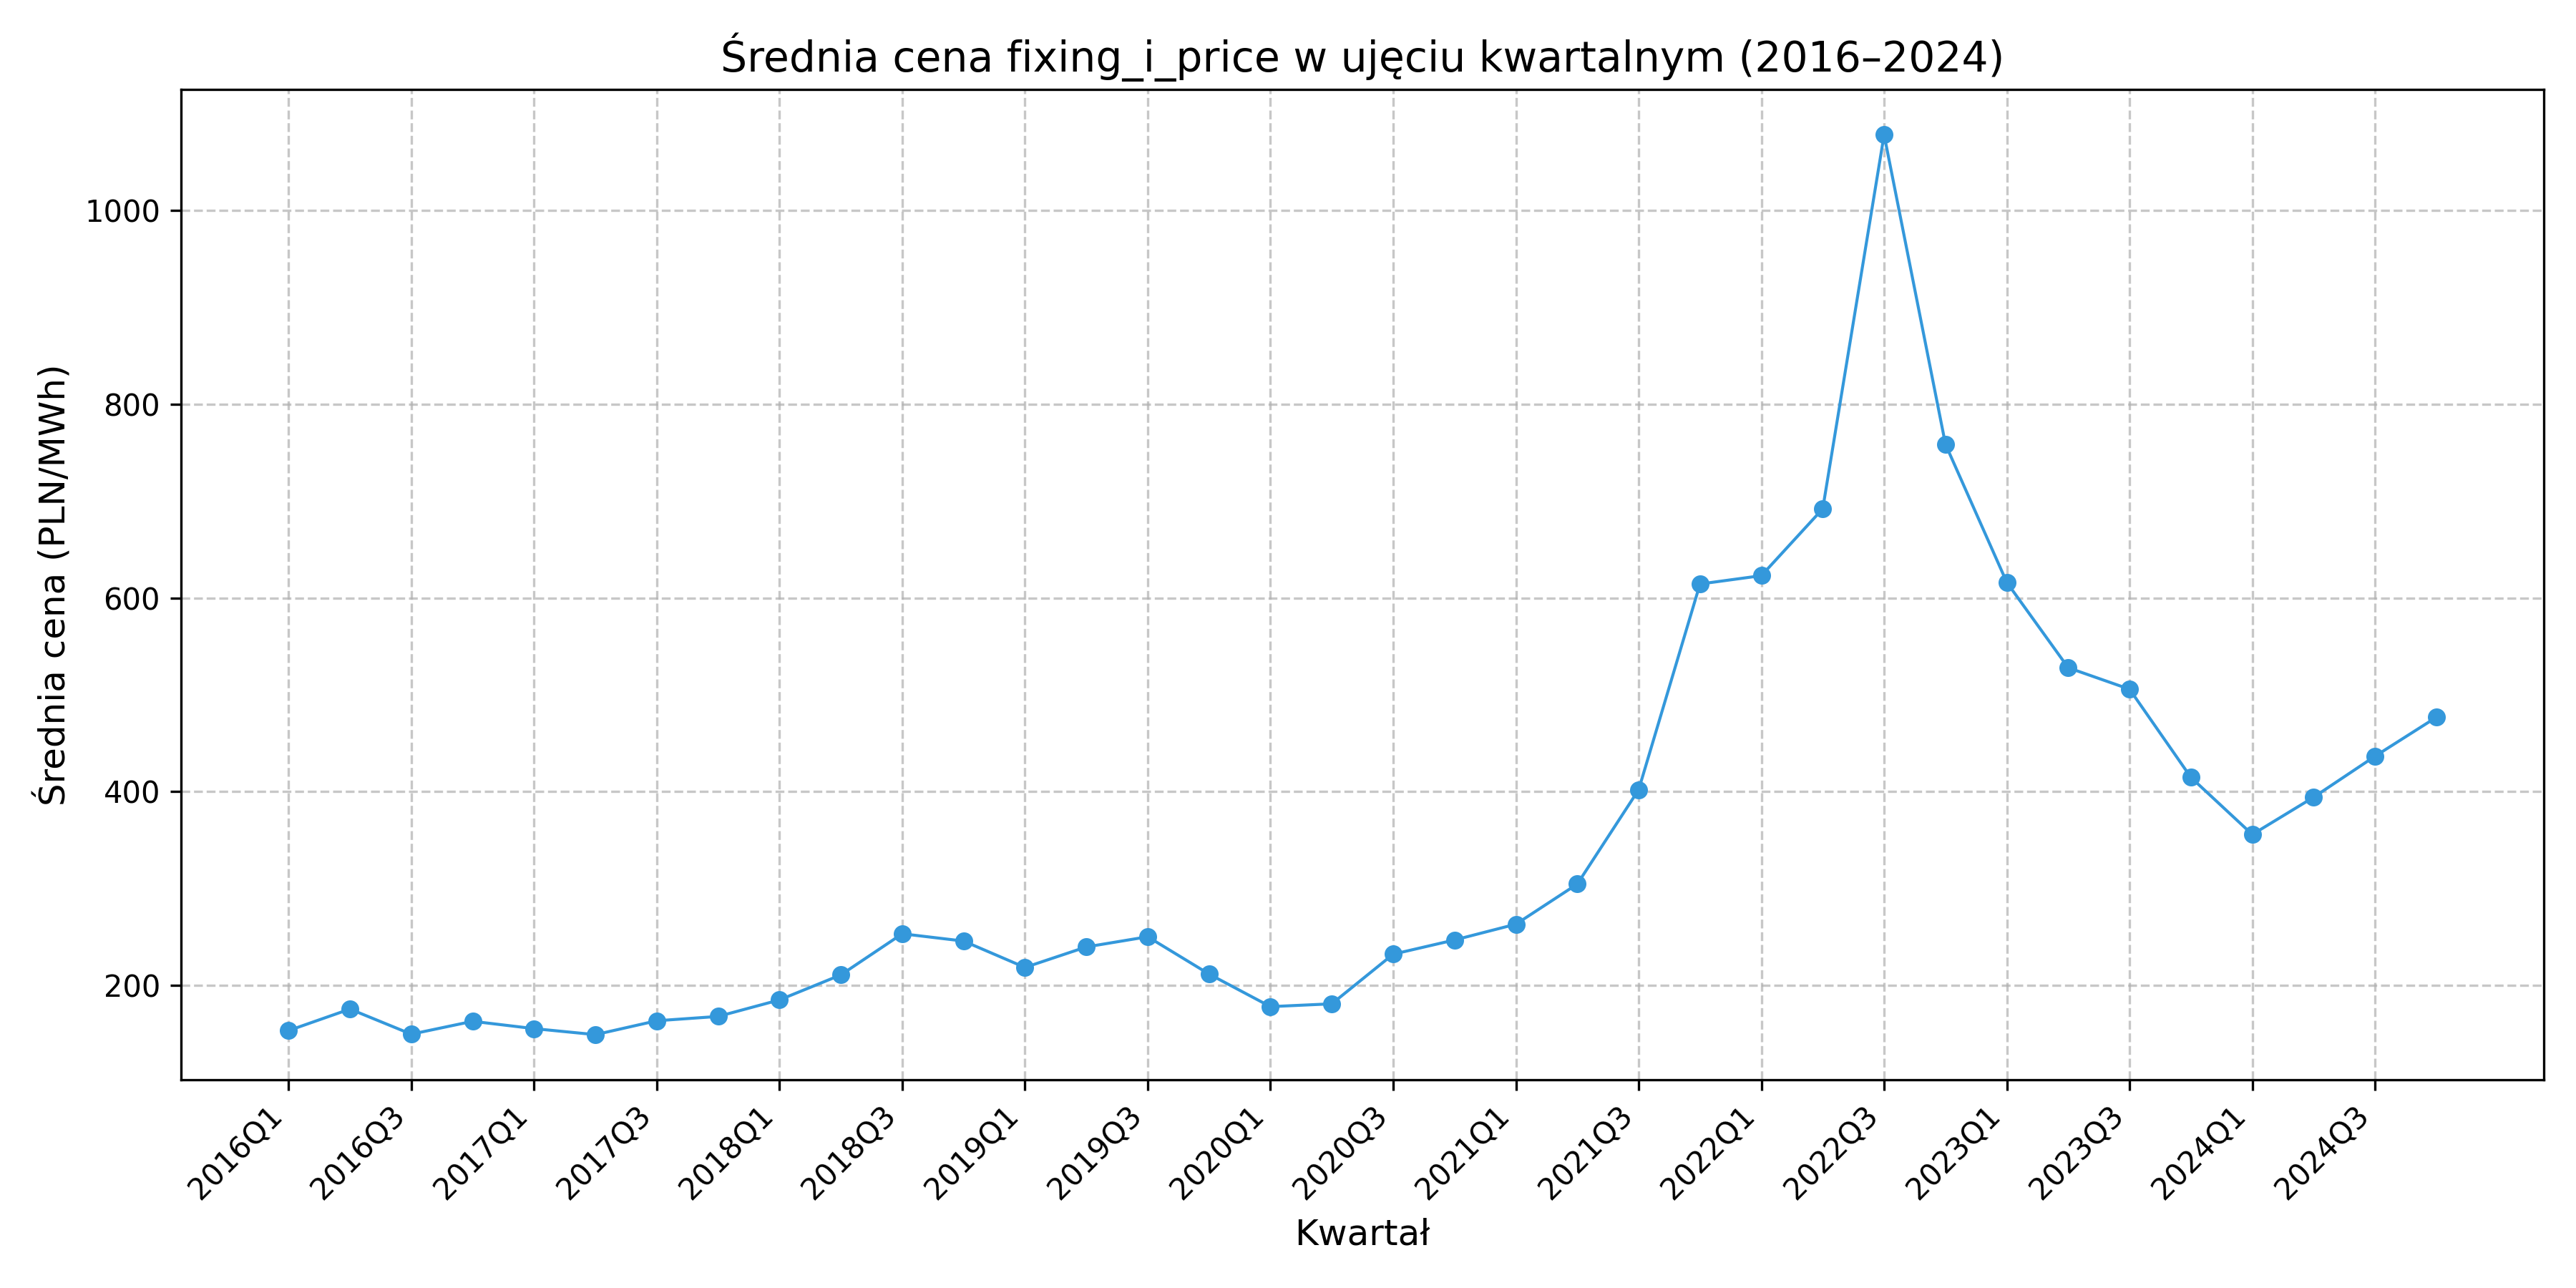
\includegraphics[width=\textwidth]{../plots/quarterly_fixing_i_price.png}
    \caption{Zmienność cen energii elektrycznej na RDN w latach 2016-2023. Opracowanie własne na podstawie danych instrat.}
    \label{fig:fixing-i-price-trend}
\end{figure}

Wyraźnie widoczna jest różnica w poziomie cen w różnych okresach: od 2016 do Q4 roku 2020 ceny były stosunkowo stabilne, oscylując w przedziale 100-300 PLN/MWh. Sytuacja zmieniła się w 2020 roku, gdy zaczęły pojawiać się pierwsze skoki cenowe z powodu poważnych obostrzeń z powodu pandemii, a w 2022 roku, w wyniku kryzysu energetycznego wywołanego wojną na Ukrainie i ograniczeniami w dostawach paliw kopalnych, ceny osiągnęły rekordowe poziomy. Pierwszy okres zostanie określony jako okres stabilności cenowej, a drugi jako okres skoków cenowych. Drugi z okresów pokazuje, jak niekorzystne sytuacje gospodarcze mogą wpływać na dynamikę cen energii, co ma istotne implikacje dla modelowania i prognozowania.

\begin{figure}
    \centering
    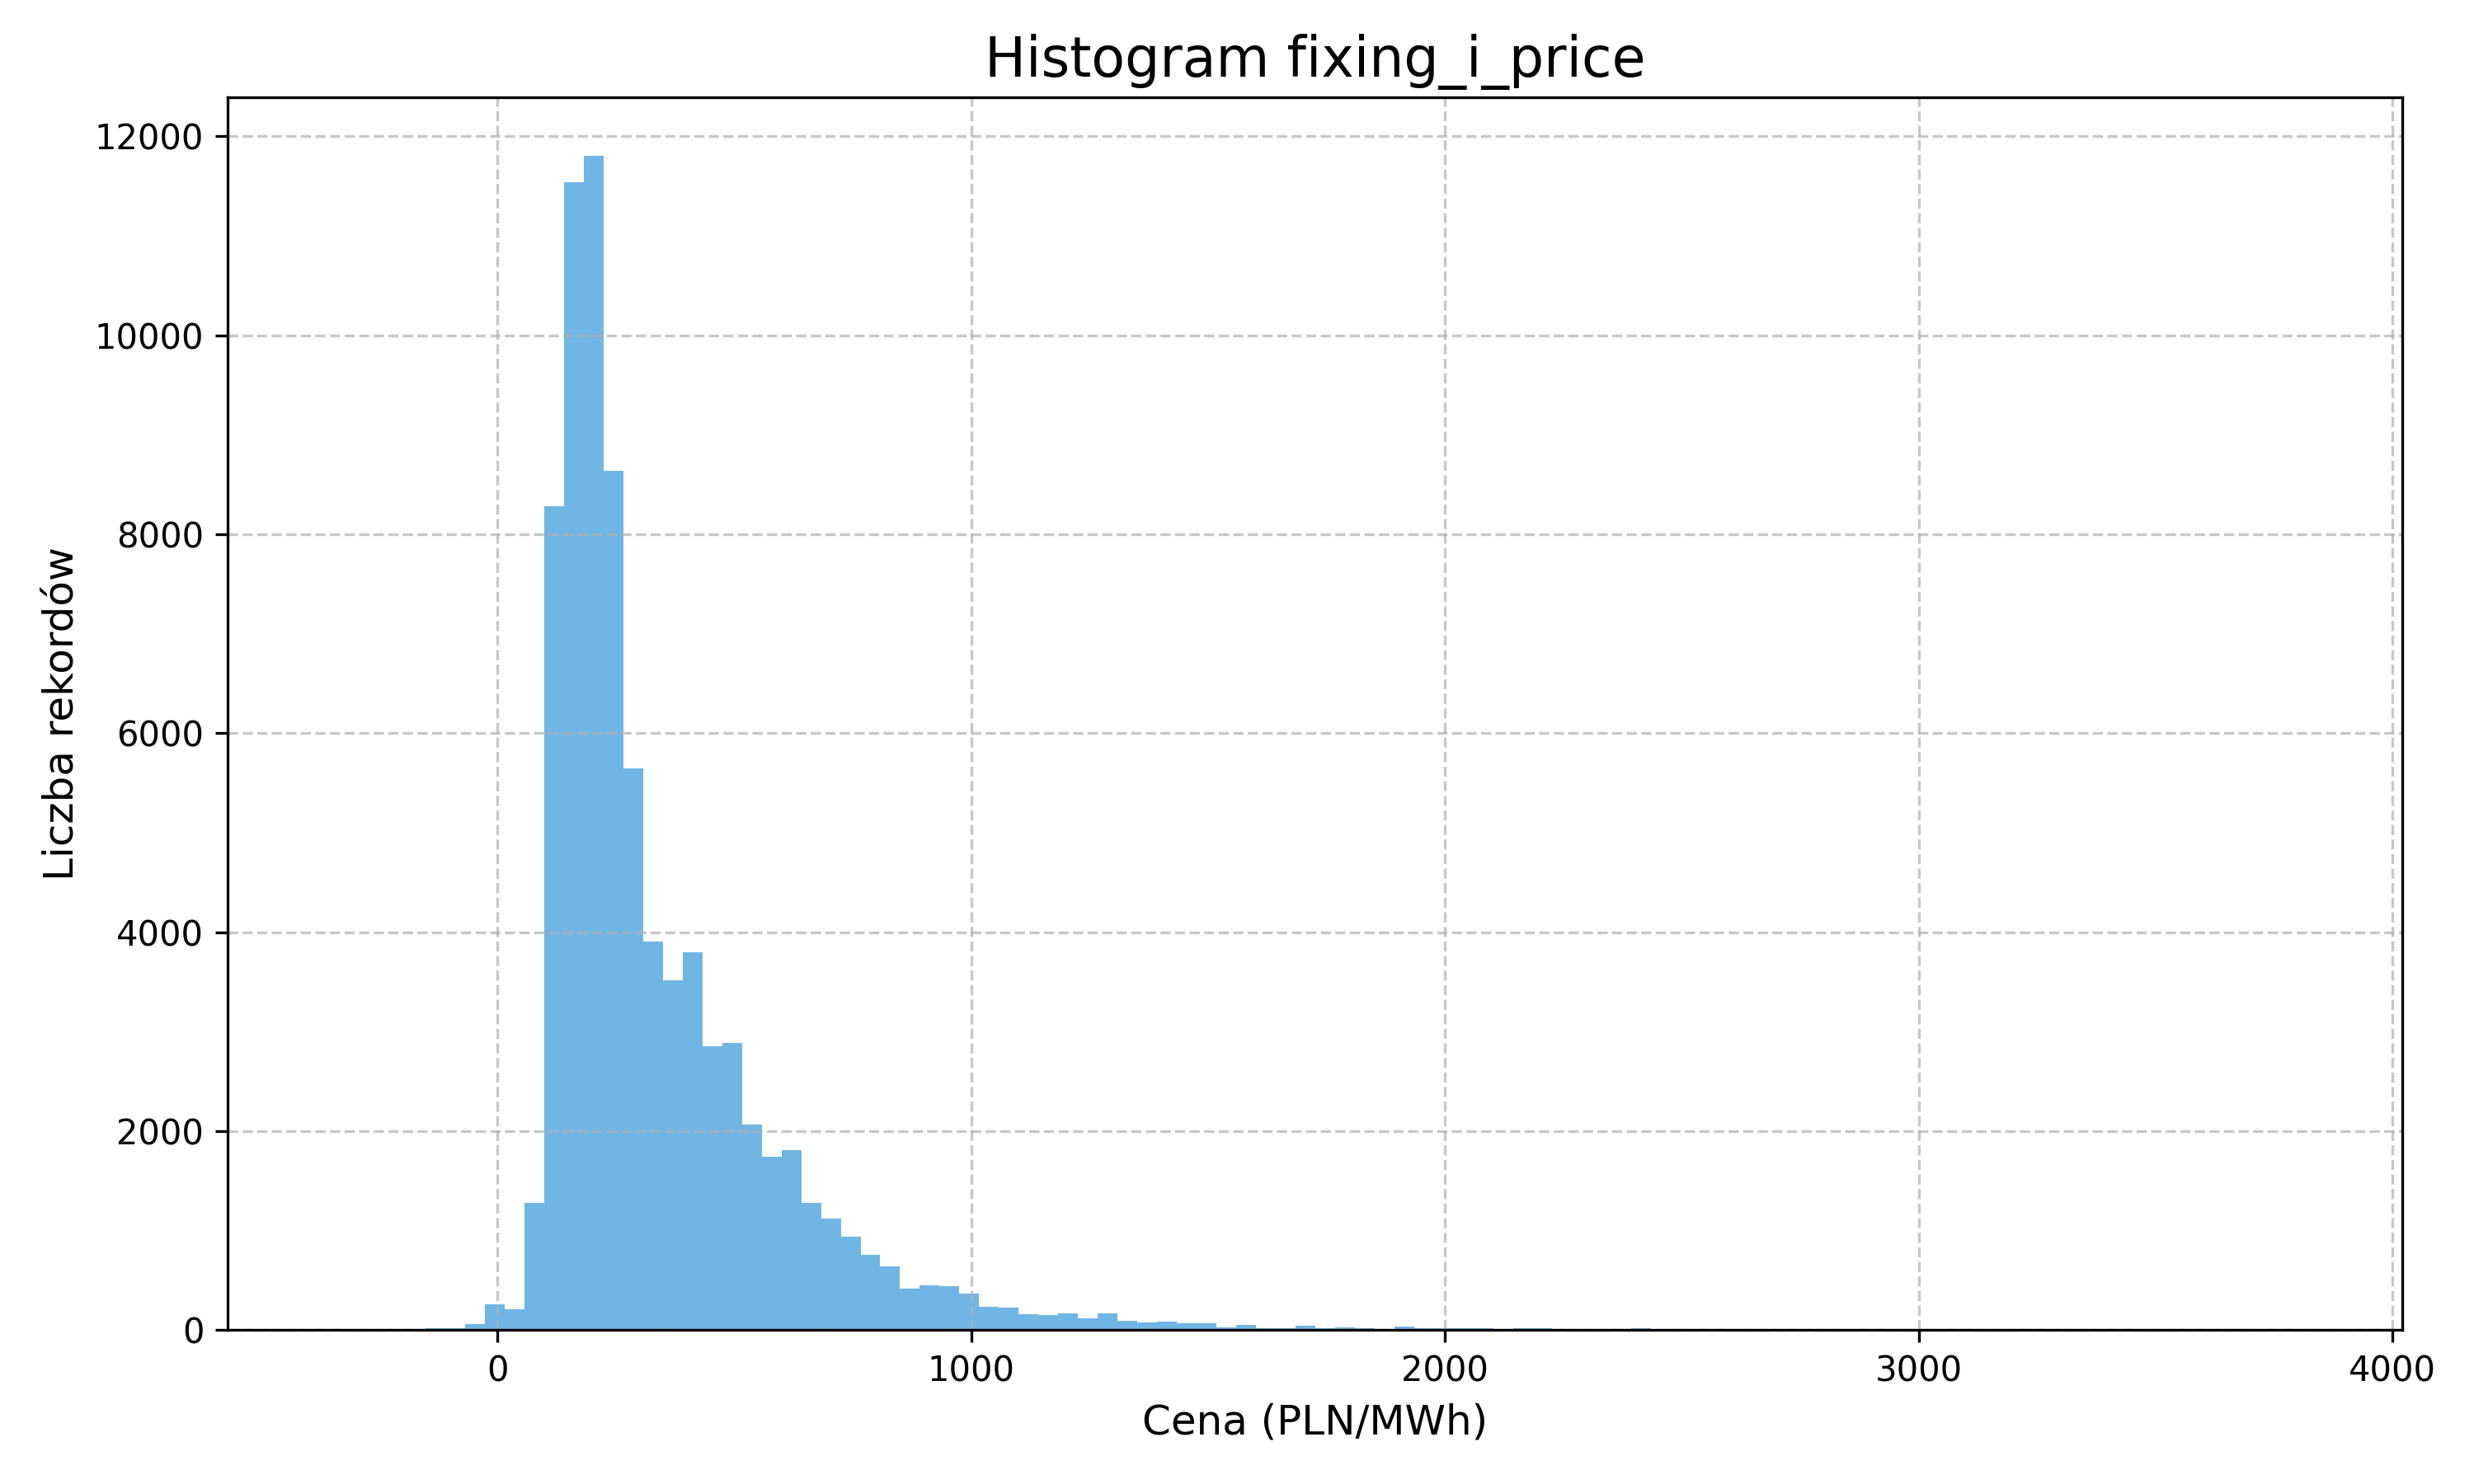
\includegraphics[width=\textwidth]{../plots/fixing_i_price_histogram.png}
    \caption{Histogram rozkładu zmiennej fixing\_i\_price. Opracowanie własne na podstawie danych instrat.}
    \label{fig:fixing-i-price-histogram}
\end{figure}

Rysunek \ref{fig:fixing-i-price-histogram} przedstawia histogram rozkładu zmiennej \texttt{fixing\_i\_price}. Rozkład jest wyraźnie asymetryczny, z długim prawym ogonem, co odzwierciedla występowanie skoków cenowych, takich jak te w 2022 roku. Ujemne ceny, choć rzadkie (ok. 0,4\% rekordów), są widoczne w lewej części histogramu, co potwierdza specyficzne cechy danych i rynku.

\section{Zbiór zmiennych niezależnych}
W niniejszej pracy wykorzystano różnorodne zmienne niezależne, które można podzielić na kilka kategorii. Obejmują one dane pogodowe, zapotrzebowanie, straty sieciowe, bilanse wymiany transgranicznej, dane o produkcji energii przez poszczególne typy generatorów, ceny paliw kopalnych, emisji CO$_2$ i inne. Wybór tych zmiennych oparty jest na ich potencjalnym wpływie na ceny energii elektrycznej. Poniżej przedstawiono szczegółowy opis każdej z kategorii zmiennych niezależnych, które zostały uwzględnione w analizie.

\subsection{Dane pogodowe}
Pierwotnie zbiór danych miał być zestawiony z danych dostępnych za pomocą oficjalnej strony Instytutu Meteorologii i Gospodarki Wodnej, natomiat dostępne dane historyczne z lat 2016-2023 mają ograniczoną rozdzielczość. Dane IMGW są zbierane przez wiele stacji meteorologicznych rozproszonych po całym kraju, ale jedynie w godzinach 6:00, 12:00 oraz 18:00. Aproksymować dane pogodowe w godzinach nocnych jest zadaniem nie do wykonania, szczególnie w przypadku sezonów zimowych, gdzie temperatura w nocy może drastycznie spadać w ciągu godziny. Z tego powodu jako źródło danych pogodowych wykorzystano stronę open-meteo \cite{METEO}. Jest to strona, która zbiera dane godzinowe z dokładnością do jednego kilometra. Dostępne są dane pogodowe dla dowolnego okresu czasu i lokalizacji.

Dane pogodowe zostały pobrane dla czterech lokalizacji w Polsce: Warszawy (WAW), Koszalina (KSZ), Krakowa (KRK) i Babimostu (BAB). Wybór miast został podyktowany ich zróżnicowaniem geograficznym i klimatycznym, co pozwala uwzględnić regionalne różnice w warunkach pogodowych wpływających na produkcję i zapotrzebowanie na energię. 

Warszawa, jako stolica i największe miasto Polski, reprezentuje centralny region kraju o wysokim zapotrzebowaniu na energię, szczególnie w okresach zimowych i letnich. Koszalin, położony na Pomorzu, jest kluczowy ze względu na bliskość farm wiatrowych na Morzu Bałtyckim, co czyni go istotnym punktem dla analizy produkcji energii wiatrowej. Kraków, znajdujący się w południowej Polsce, charakteryzuje się większym udziałem energii słonecznej w miksie energetycznym, a także wysokim zapotrzebowaniem na energię w sezonie grzewczym. Babimost, zlokalizowany w zachodniej Polsce, jest istotny ze względu na swoje położenie na zachodzie Polski w pobliżu granicy z Niemcami.

Parametry pogodowe zostały wybrane z uwzględnieniem ich bezpośredniego wpływu na rynek energii.\newline
Temperatura jest kluczowym czynnikiem, ponieważ bezpośrednio wpływa na zapotrzebowanie na energię. Niskie temperatury zwiększają zużycie energii na ogrzewanie, natomiast bardzo wysokie temperatury latem mogą podnosić zapotrzebowanie na klimatyzację.\newline
Udostępniona prędkość wiatru została zmierzona na wysokości 100 metrów nad powierzchnią ziemi. Taka wysokość została wybrana, ponieważ jest przeciętna dla turbin wiatrowych w Polsce, co pozwala dokładniej oszacować potencjalną produkcję energii z farm wiatrowych.\newline
Promieniowanie słoneczne jest istotnym czynnikiem dla produkcji energii z paneli fotowoltaicznych.\newline
Zachmurzenie zostało uwzględnione, ponieważ wysoki poziom zachmurzenia zmniejsza efektywność paneli słonecznych. 
Wybór tych parametrów pozwala na kompleksową analizę wpływu pogody na ceny energii na RDN.

Poniżej przedstawię wykresy dla każdego z parametrów pogodowych, które zostały uwzględnione w analizie. Wykresy przedstawiają zmienność danych pogodowych w czasie. Zachmurzenie jest wyrażone w oktantach (0-8), gdzie 0 oznacza brak zachmurzenia, a 8 oznacza całkowite zachmurzenie.

\begin{figure}[H]
    \centering
    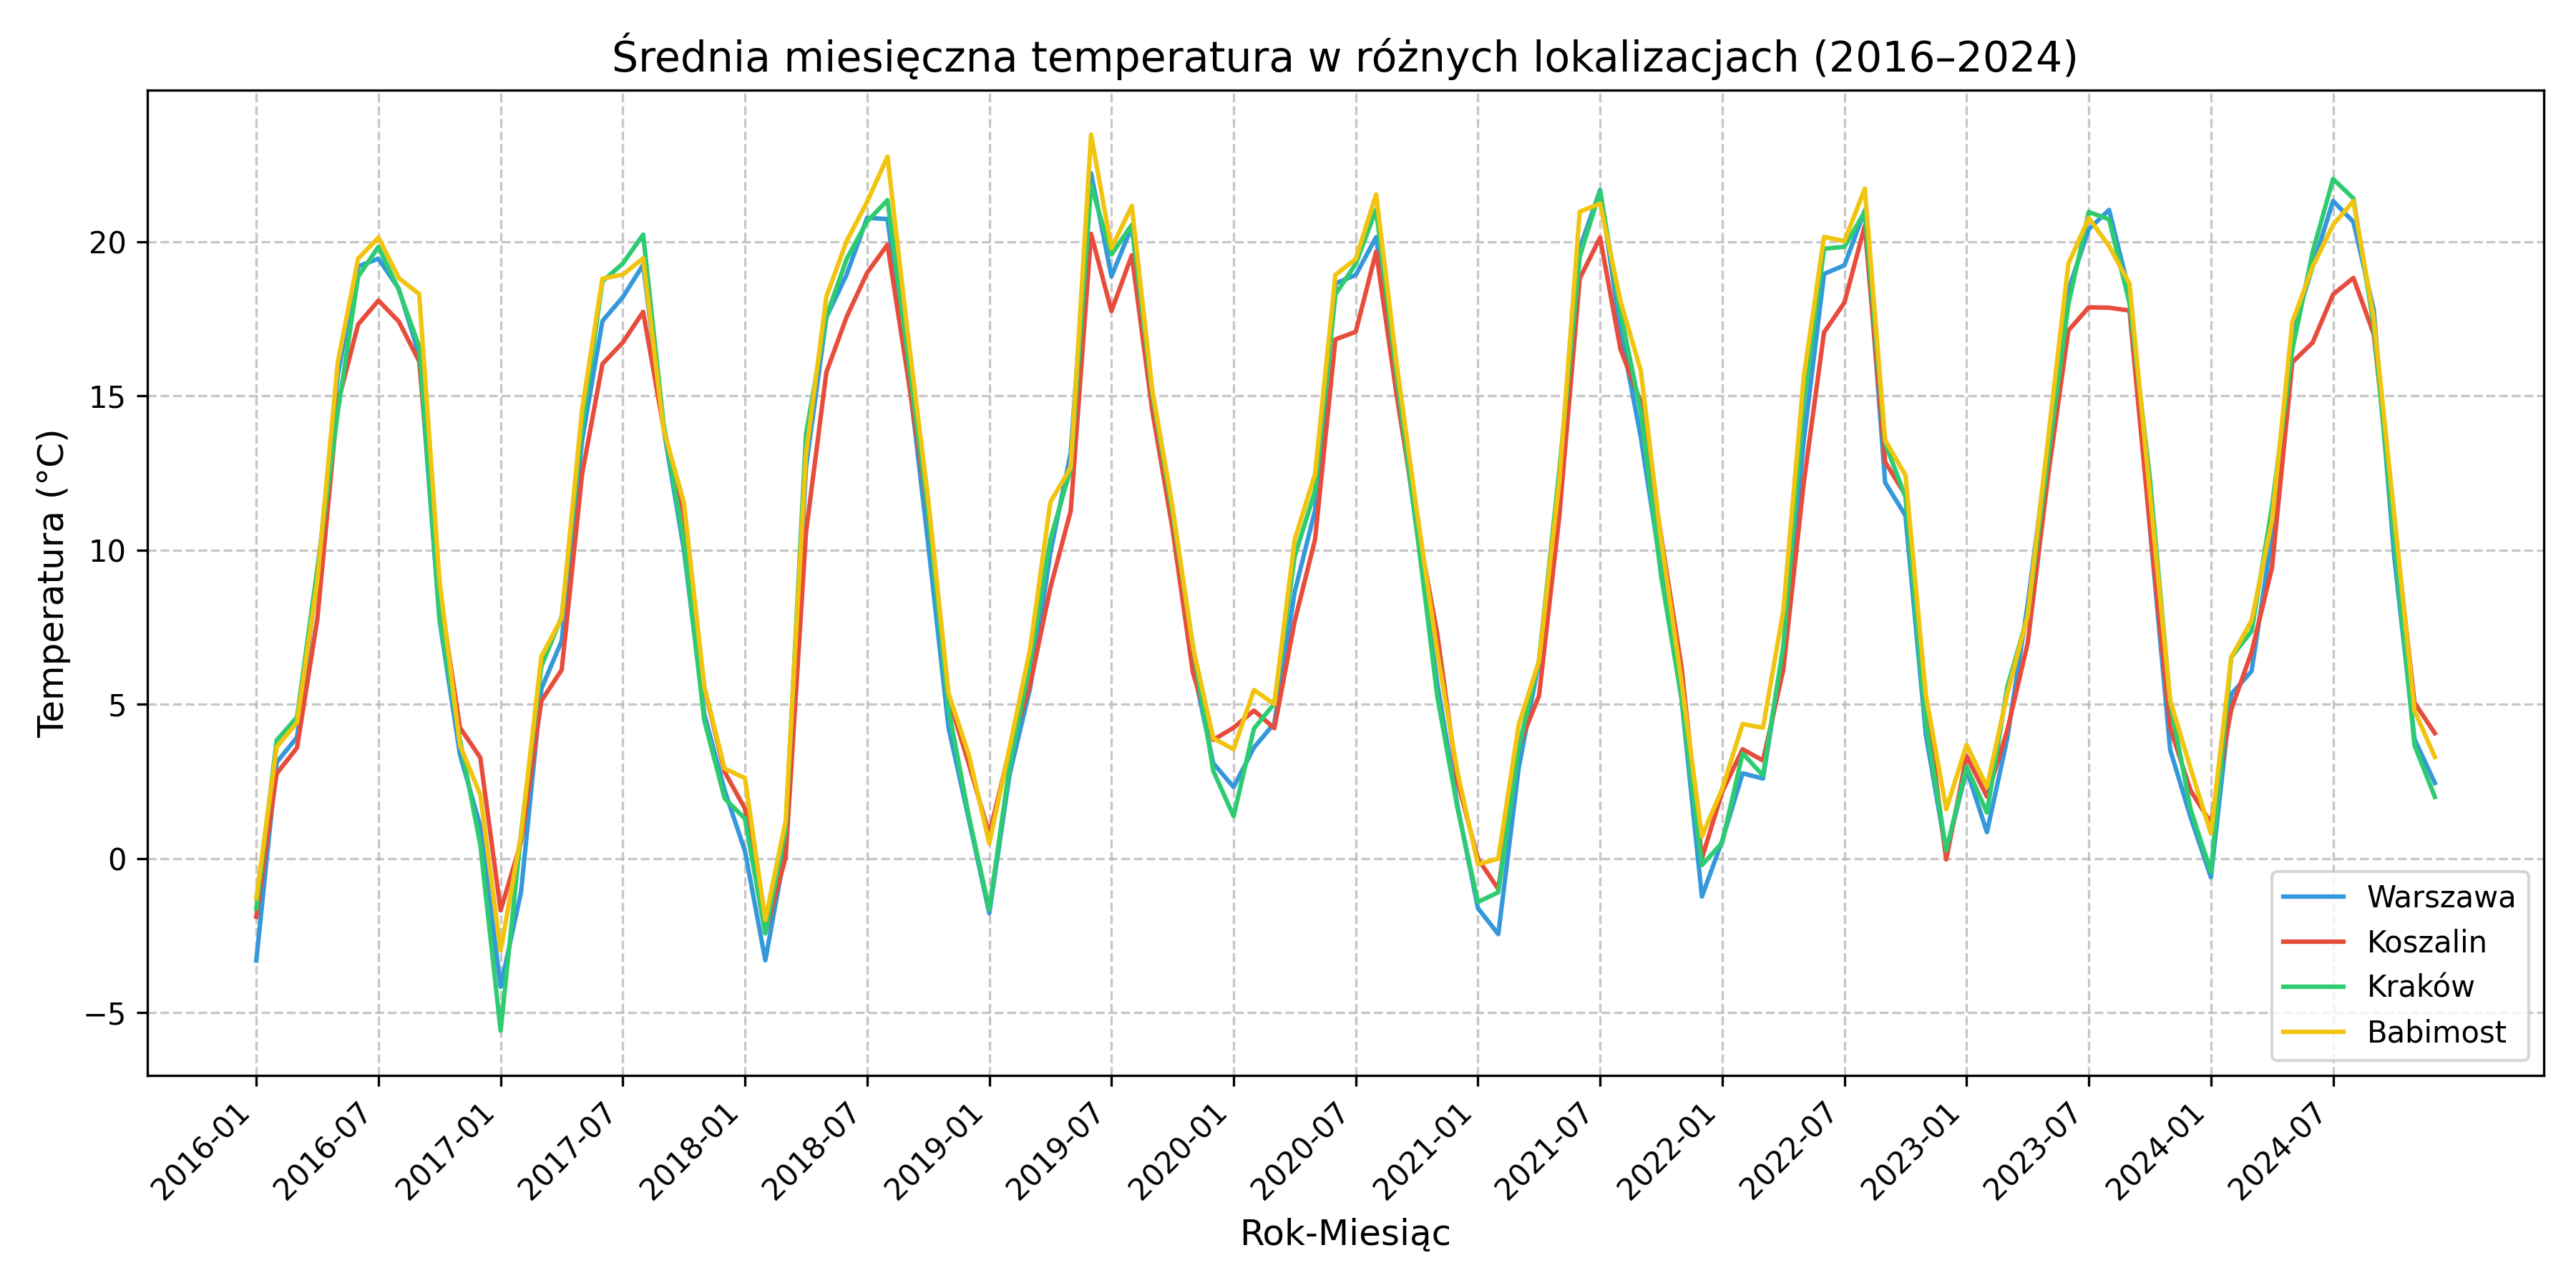
\includegraphics[width=\textwidth]{../plots/weather/temp_time_series_full.png}
    \caption{Zmienność temperatury w czasie (2016-2023). Opracowanie własne na podstawie danych open-meteo.}
    \label{fig:temp-time-series-full}
\end{figure}

\begin{figure}[H]
    \centering
    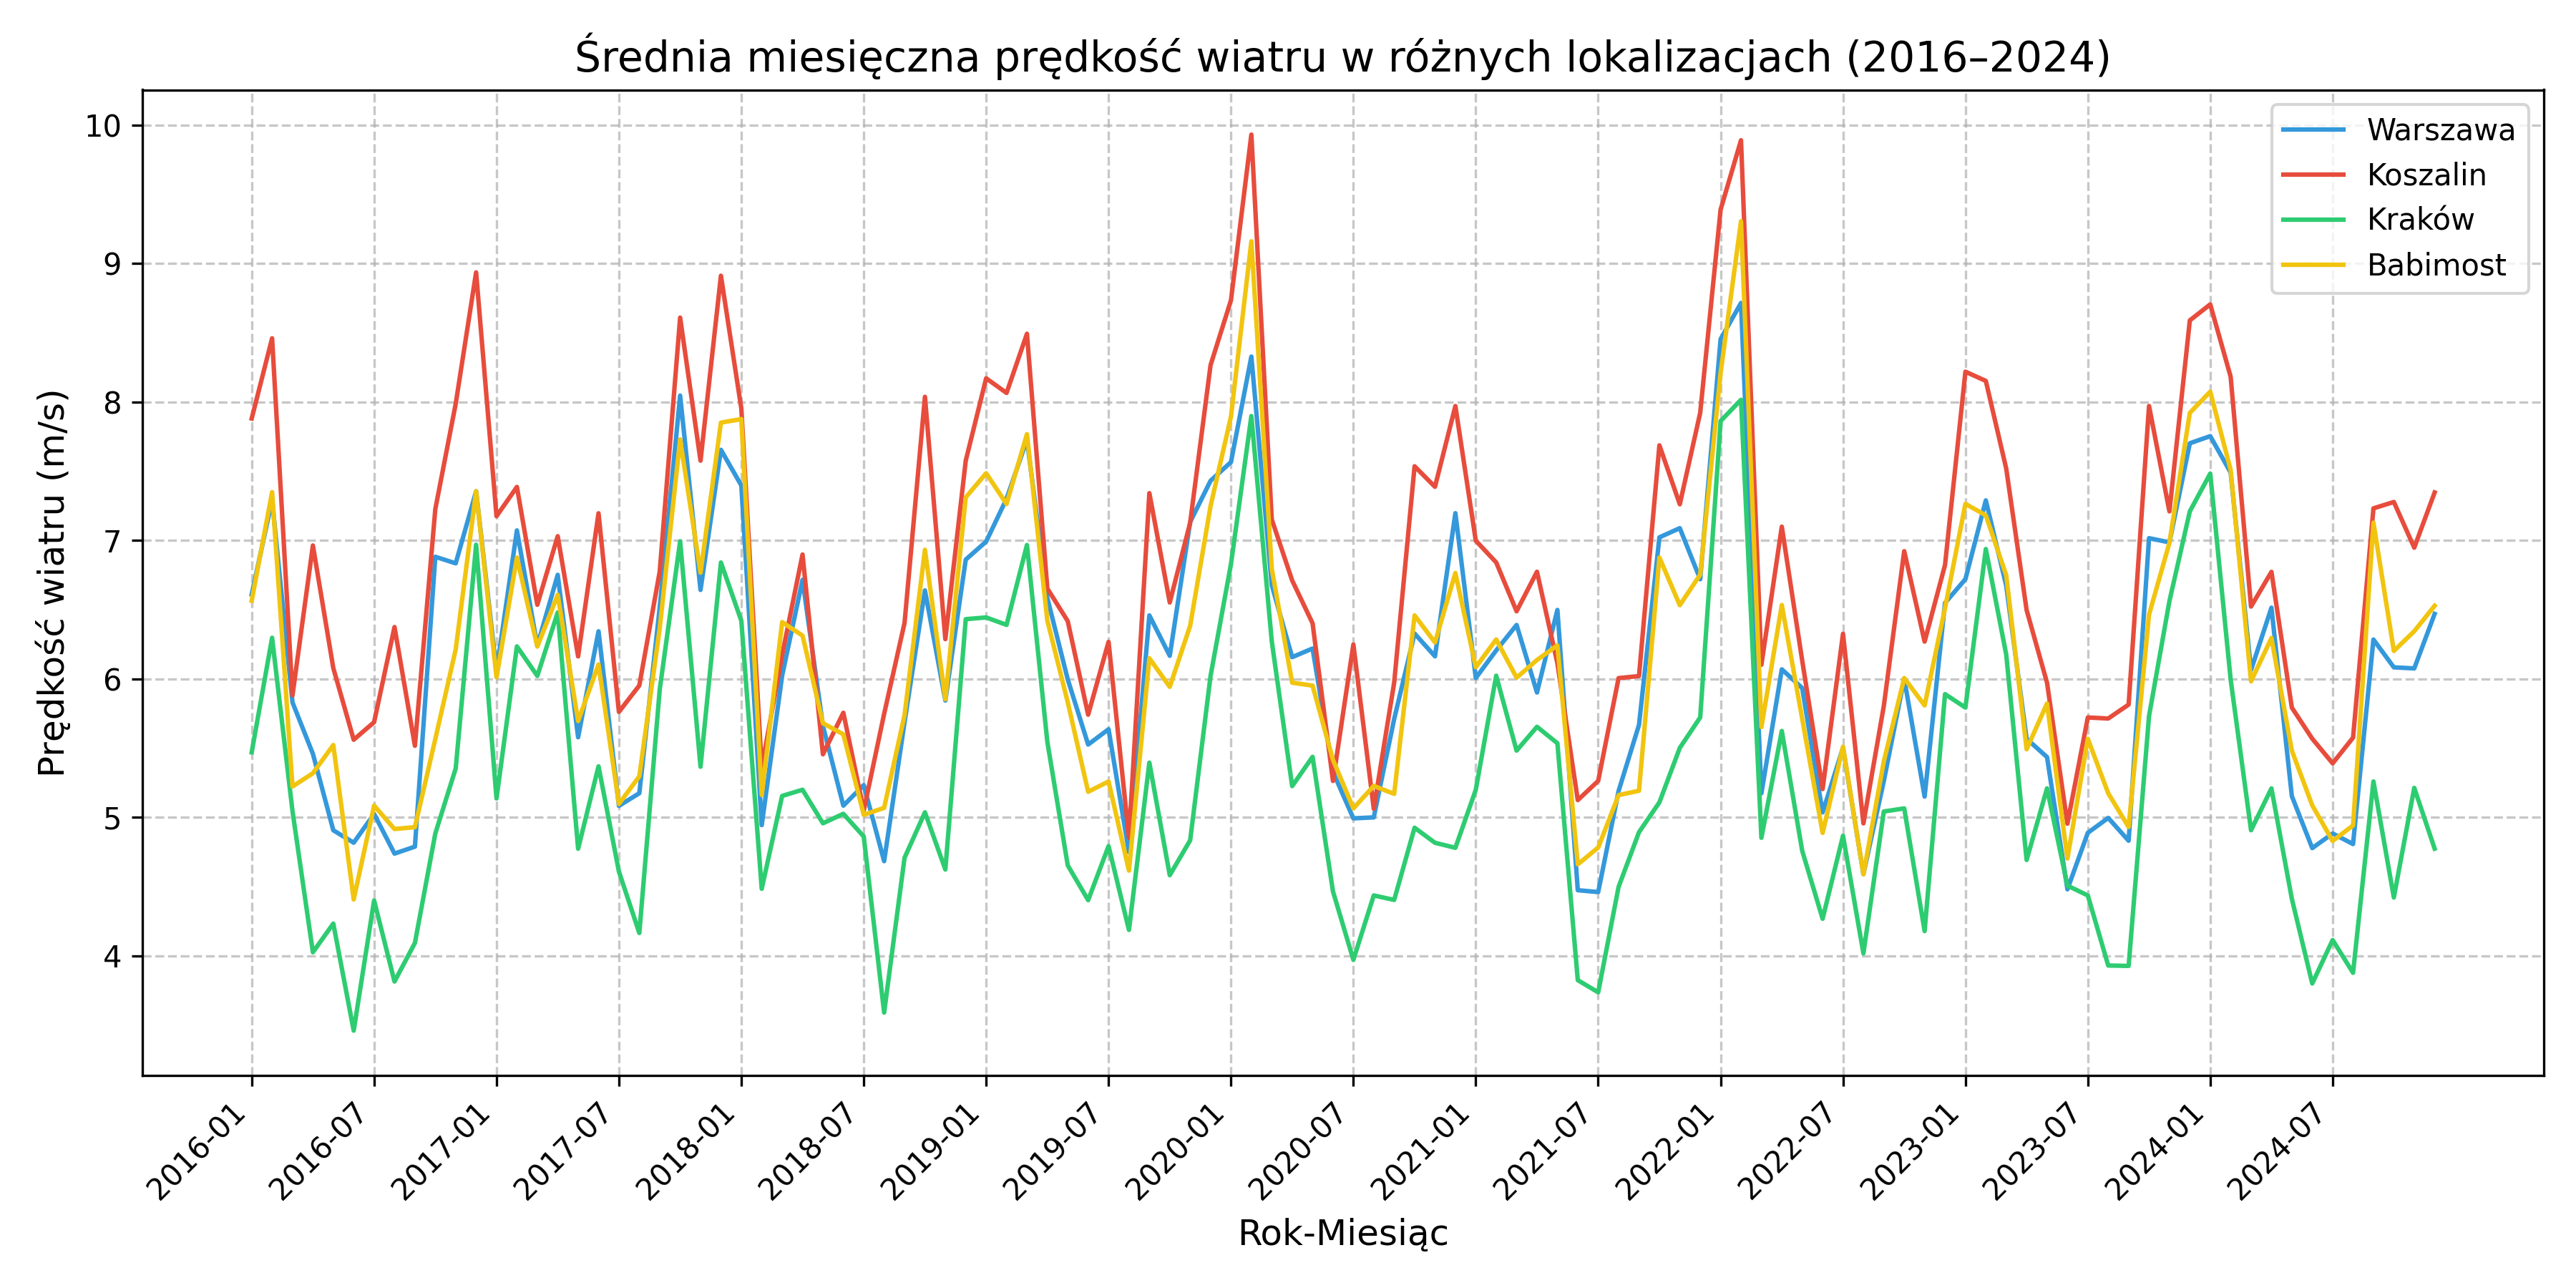
\includegraphics[width=\textwidth]{../plots/weather/wind_speed_time_series_full.png}
    \caption{Zmienność prędkości wiatru w czasie (2016-2023) Opracowanie własne na podstawie danych open-meteo.}
    \label{fig:wind-speed-time-series-full}
\end{figure}

\begin{figure}[H]
    \centering
    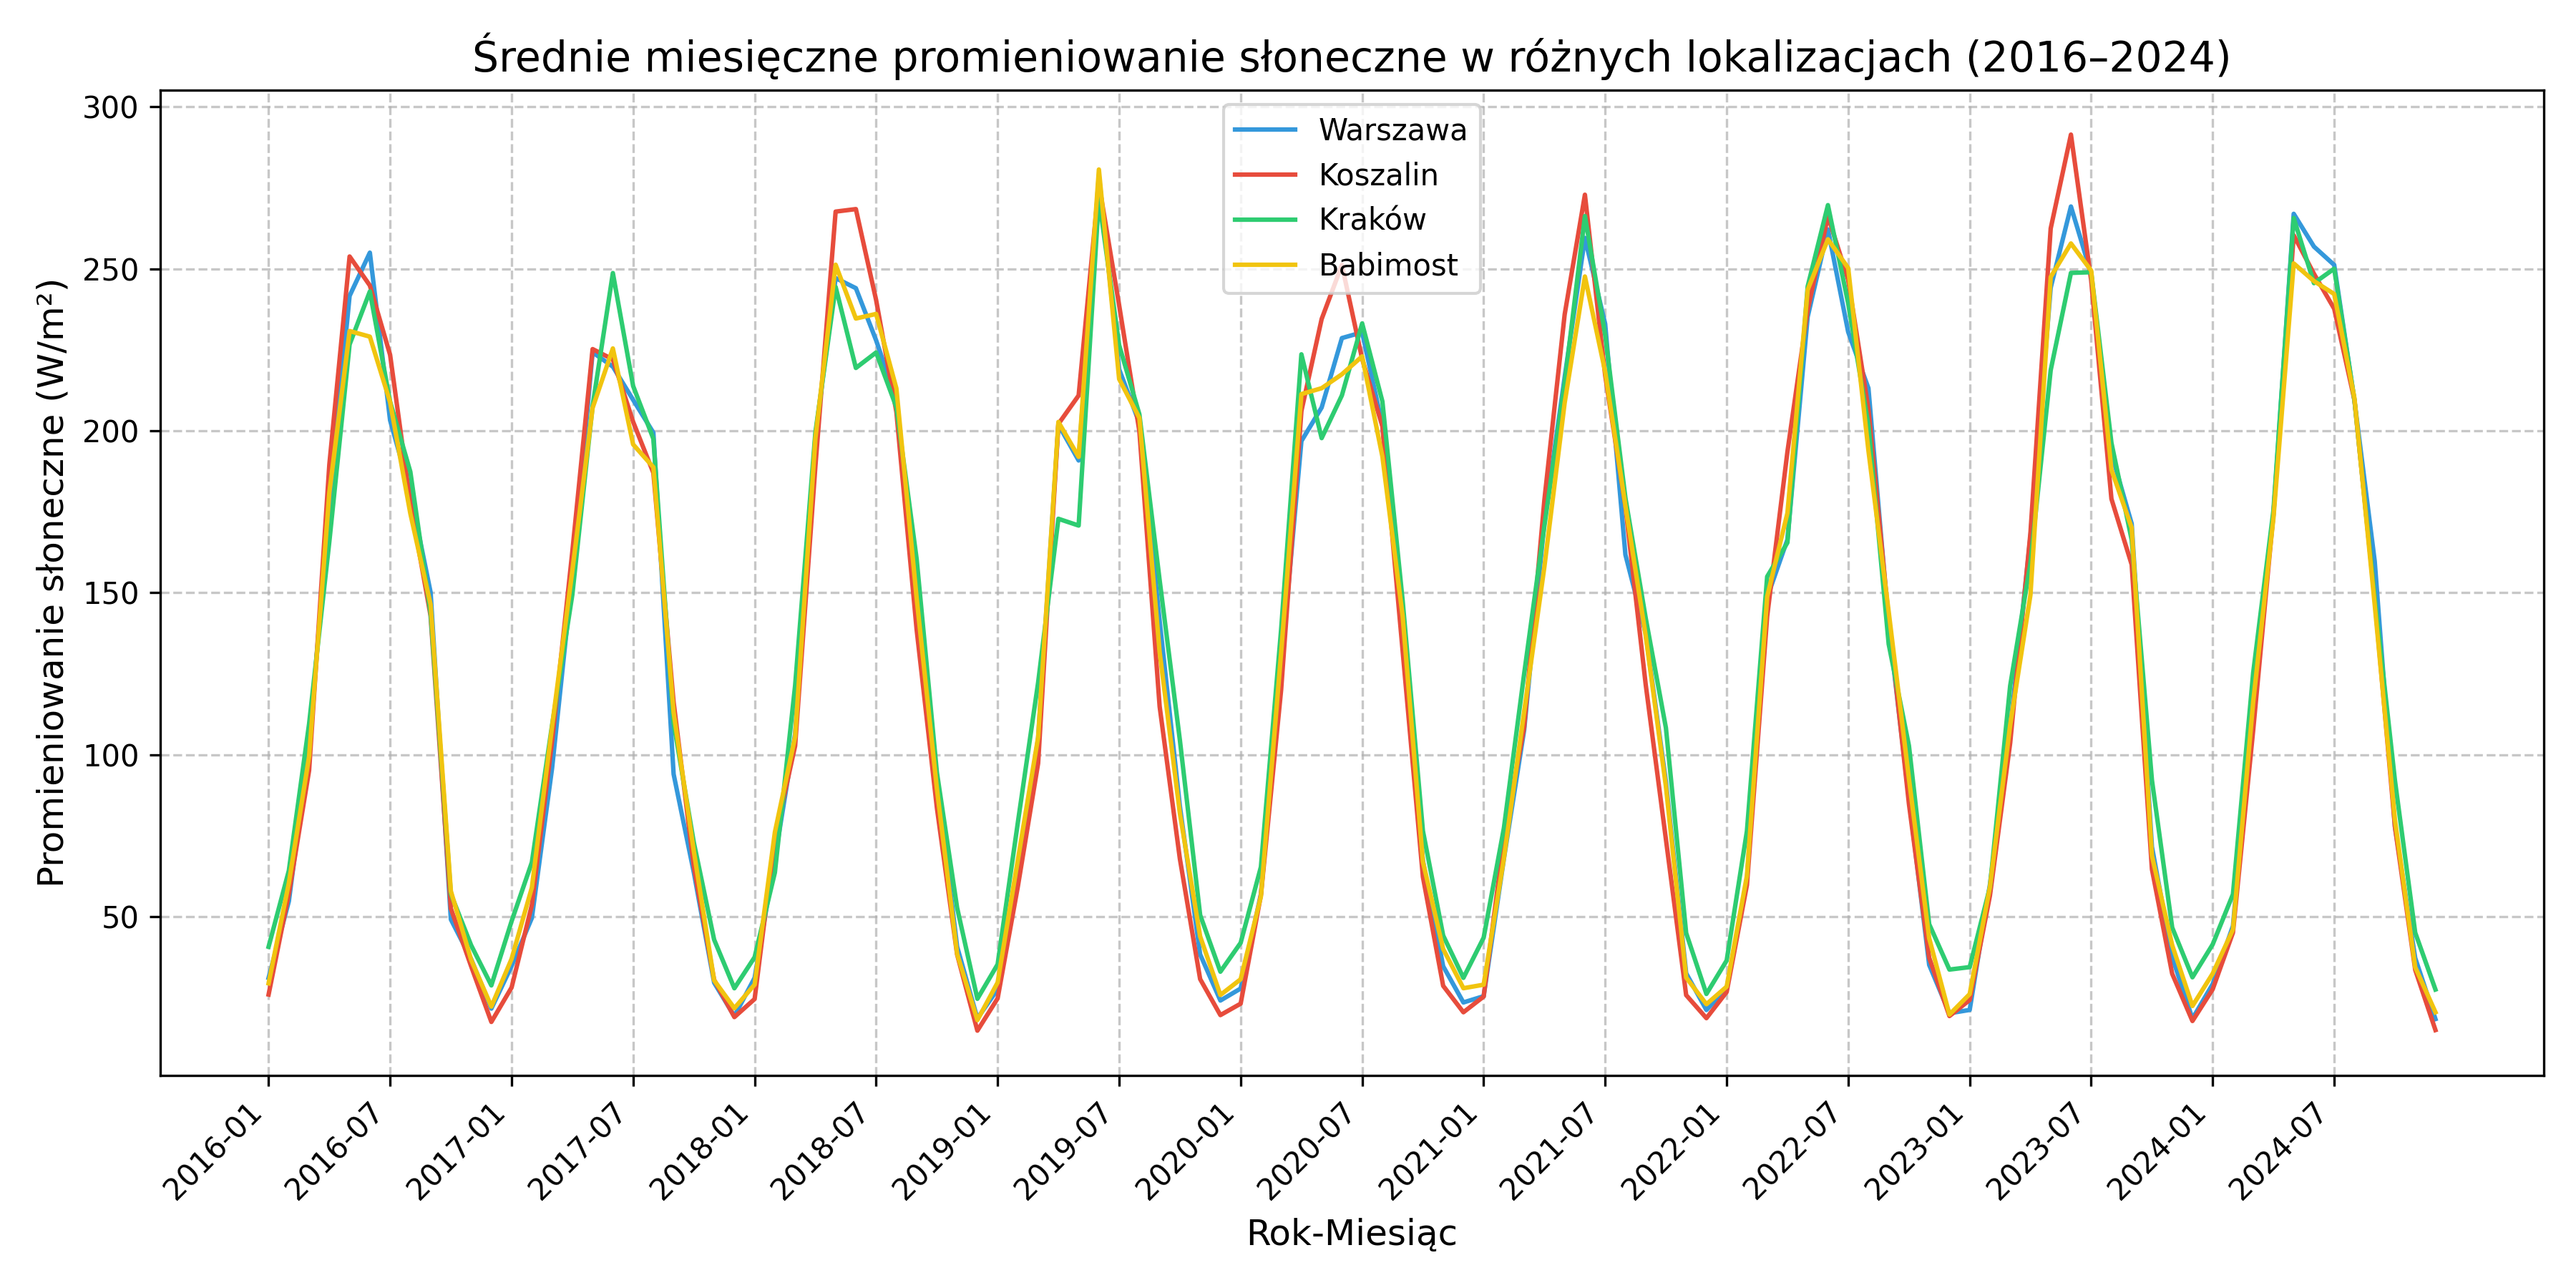
\includegraphics[width=\textwidth]{../plots/weather/solar_radiation_time_series_full.png}
    \caption{Zmienność promieniowania słonecznego w czasie (2016-2023). Opracowanie własne na podstawie danych open-meteo.}
    \label{fig:solar-radiation-time-series-full}
\end{figure}

\begin{figure}[H]
    \centering
    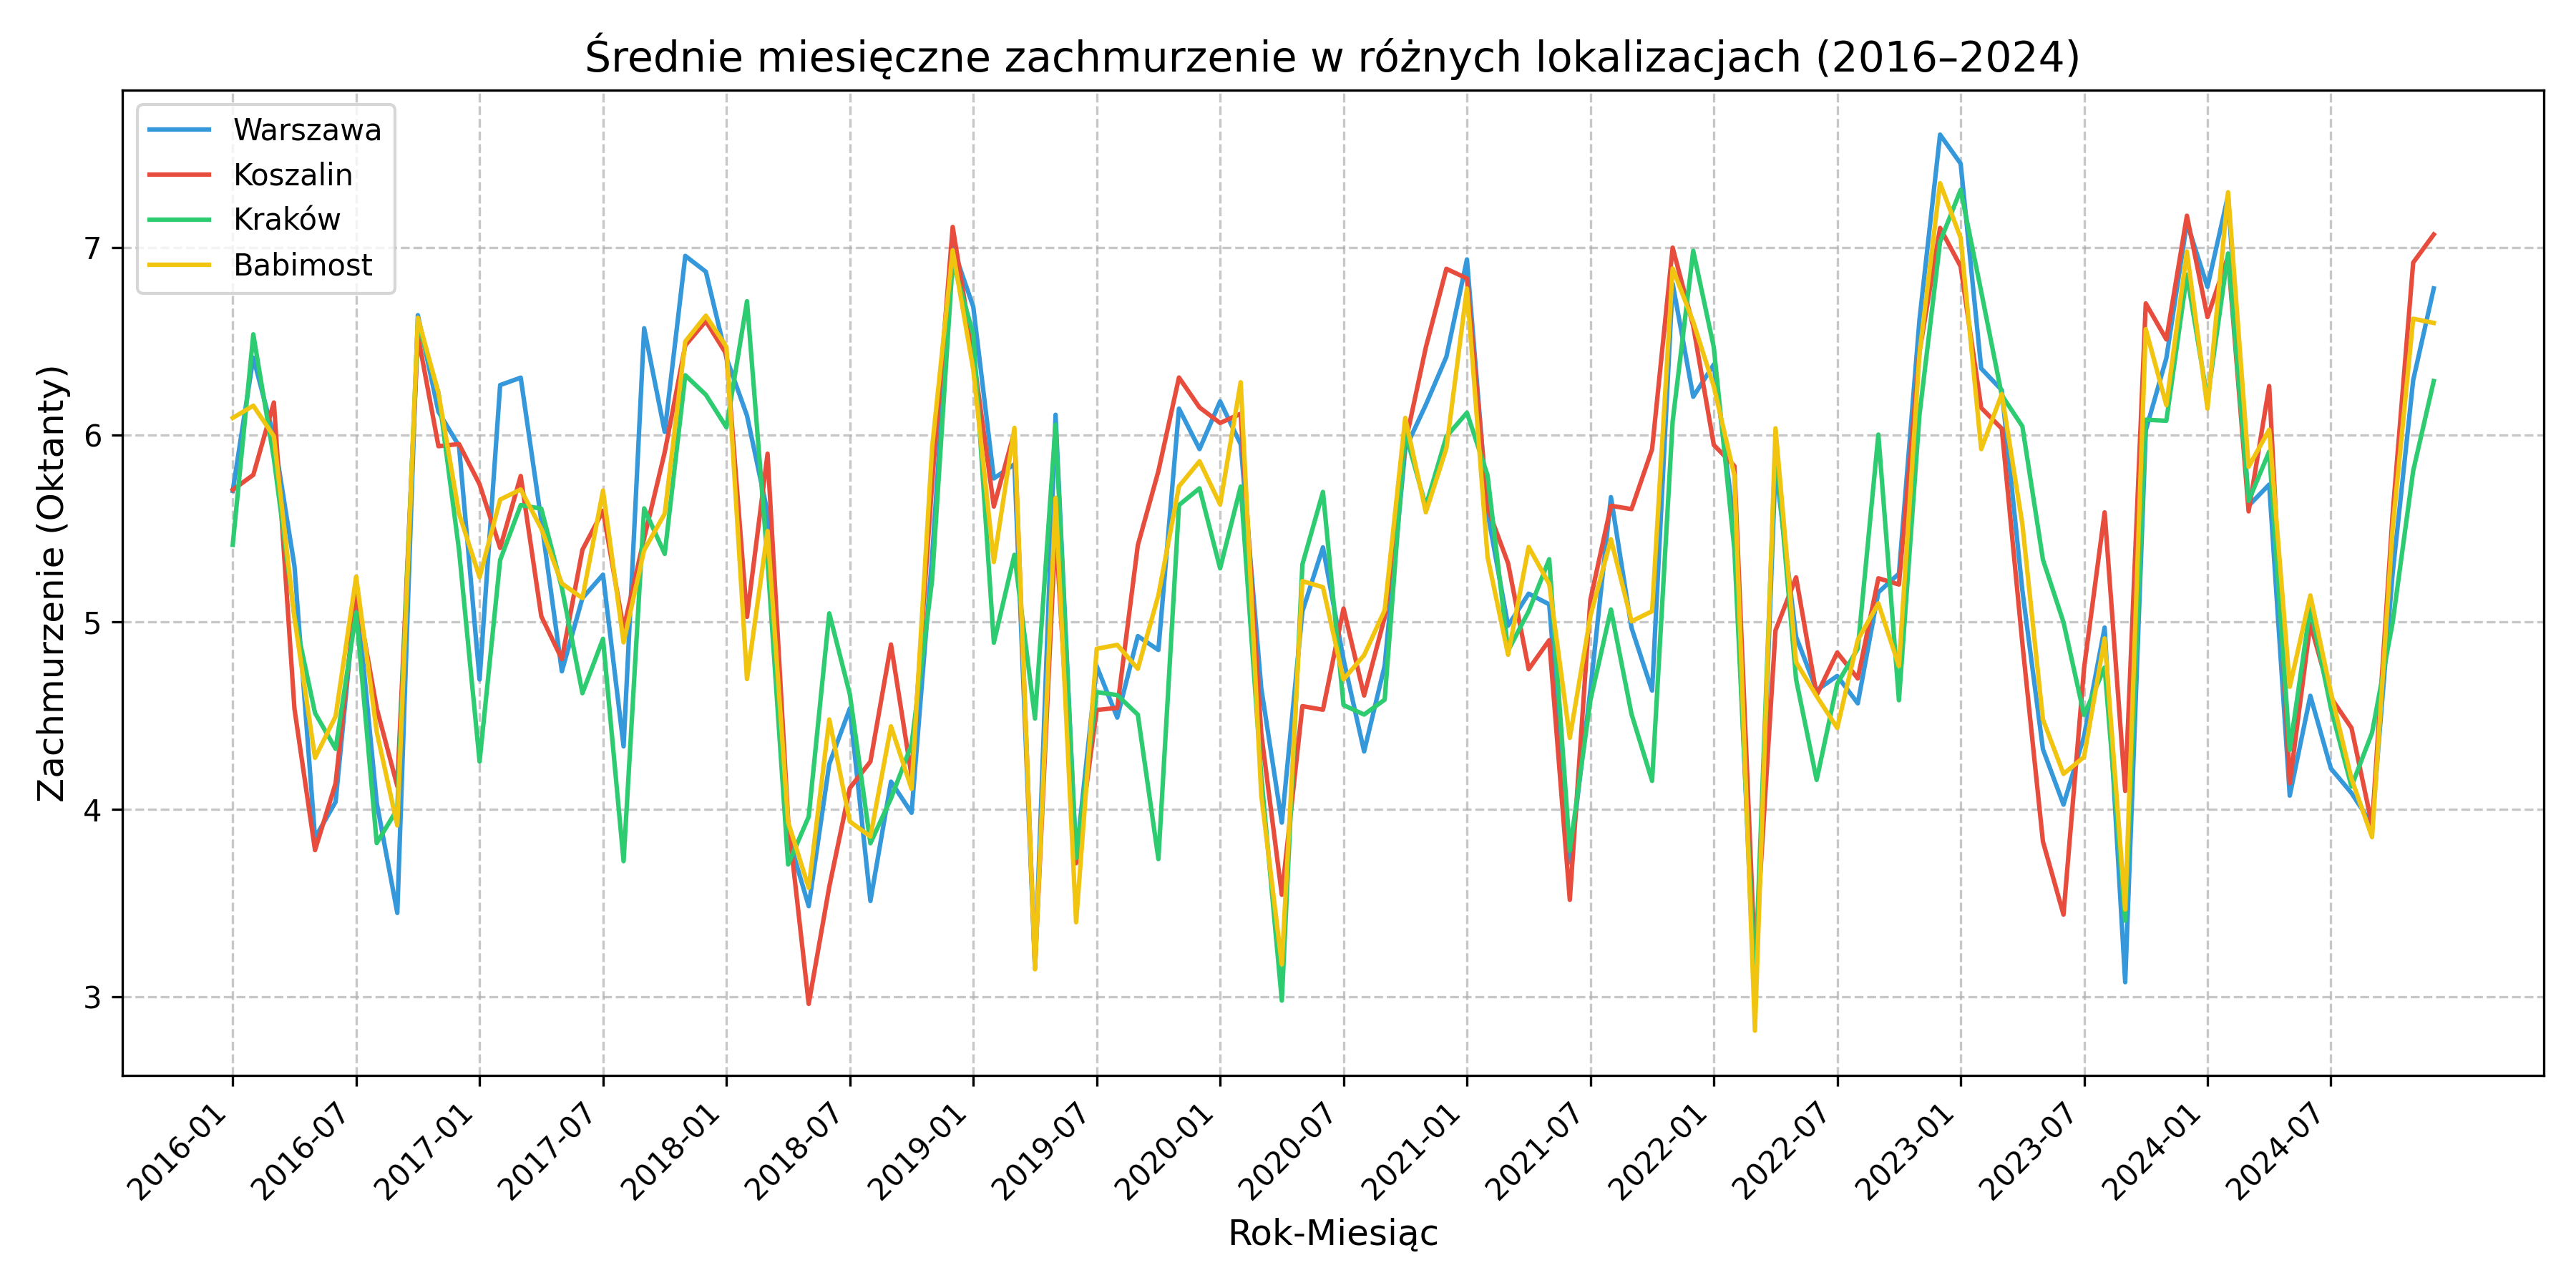
\includegraphics[width=\textwidth]{../plots/weather/cloud_cover_time_series_full.png}
    \caption{Zmienność zachmurzenia w czasie (2016-2023). Opracowanie własne na podstawie danych open-meteo.}
    \label{fig:cloud-cover-time-series-full}
\end{figure}

Każdy z wykresów przedstawia zmienność danego parametru pogodowego w wybranych lokalizacjach w przeciągu okresu badawczego. Wyraźnie widać sezonowe wahania parametrów pogodowych, co jest typowe dla klimatu Polski. Temperatura i promieniowanie słoneczne mają wyraźnie większe wartości w sezonach letnich, prędkość wiatru w sezonach zimowych, z kolei zachmurzenie ma bardziej zróżnicowany charakter.

Dodatkowo, w celu przedstawienia wahań zmiennych pogodowych w przeciągu roku, poniżej zostały załączone wykresy zmiennych pogodowych za rok 2022.
\begin{figure}[H]
    \centering
    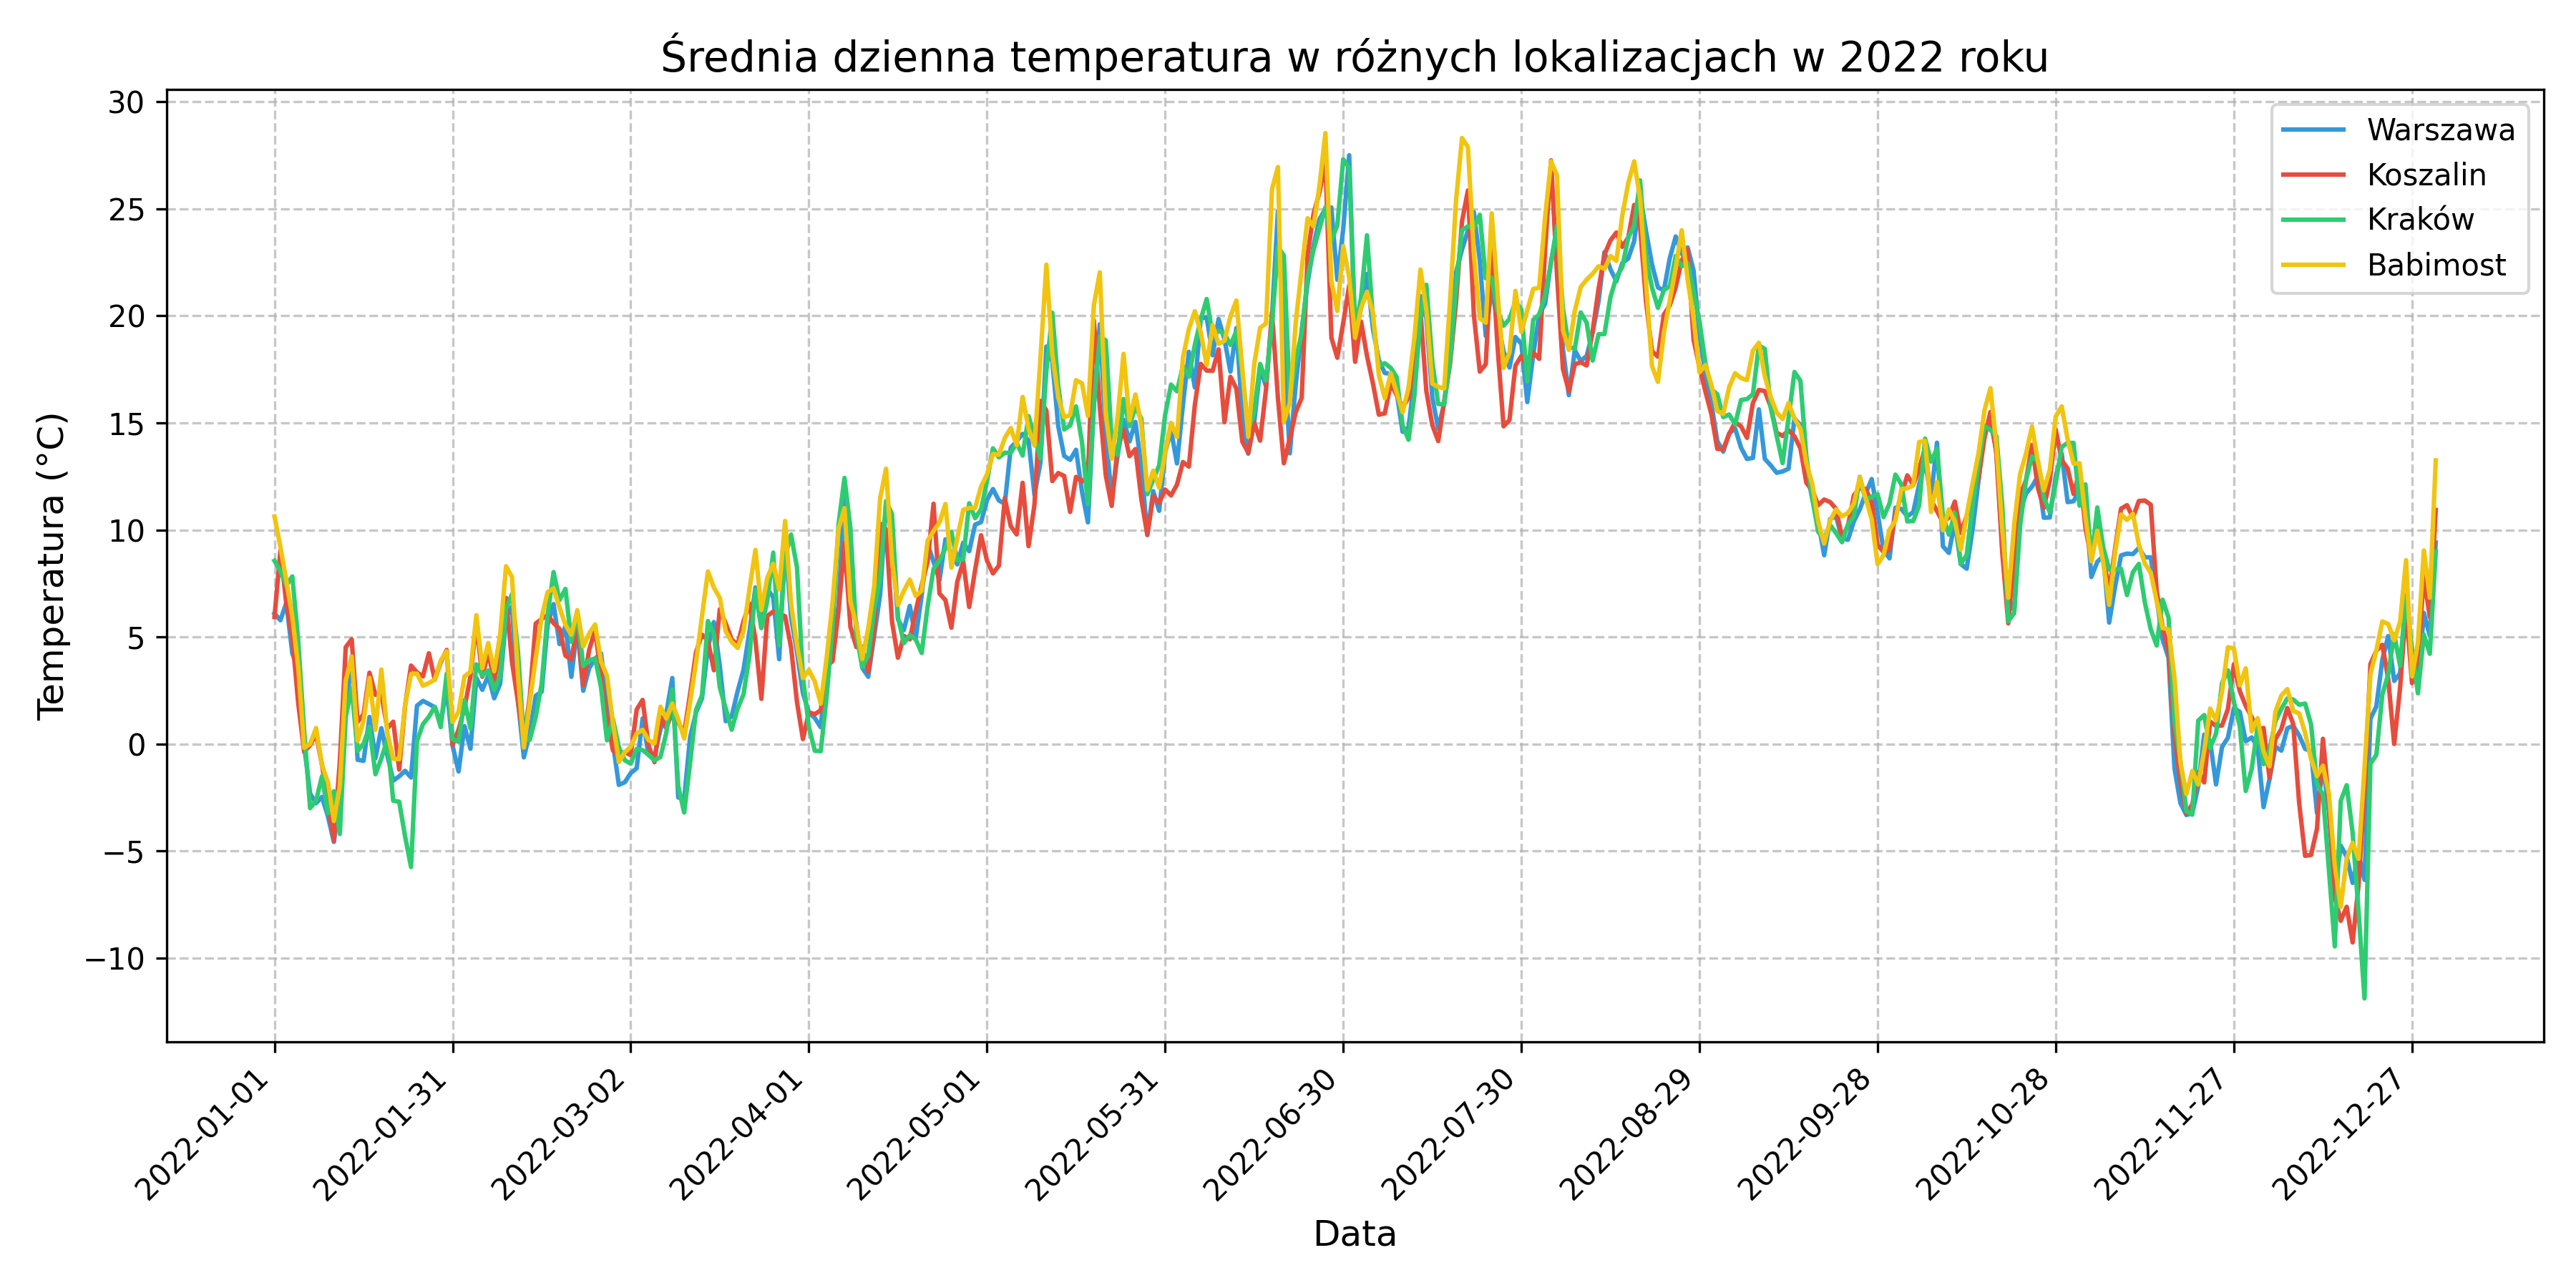
\includegraphics[width=\textwidth]{../plots/weather/temp_time_series_2022.png}
    \caption{Zmienność temperatury w czasie (2022). Opracowanie własne na podstawie danych open-meteo.}
    \label{fig:temp-time-series-2022}
\end{figure}

\begin{figure}[H]
    \centering
    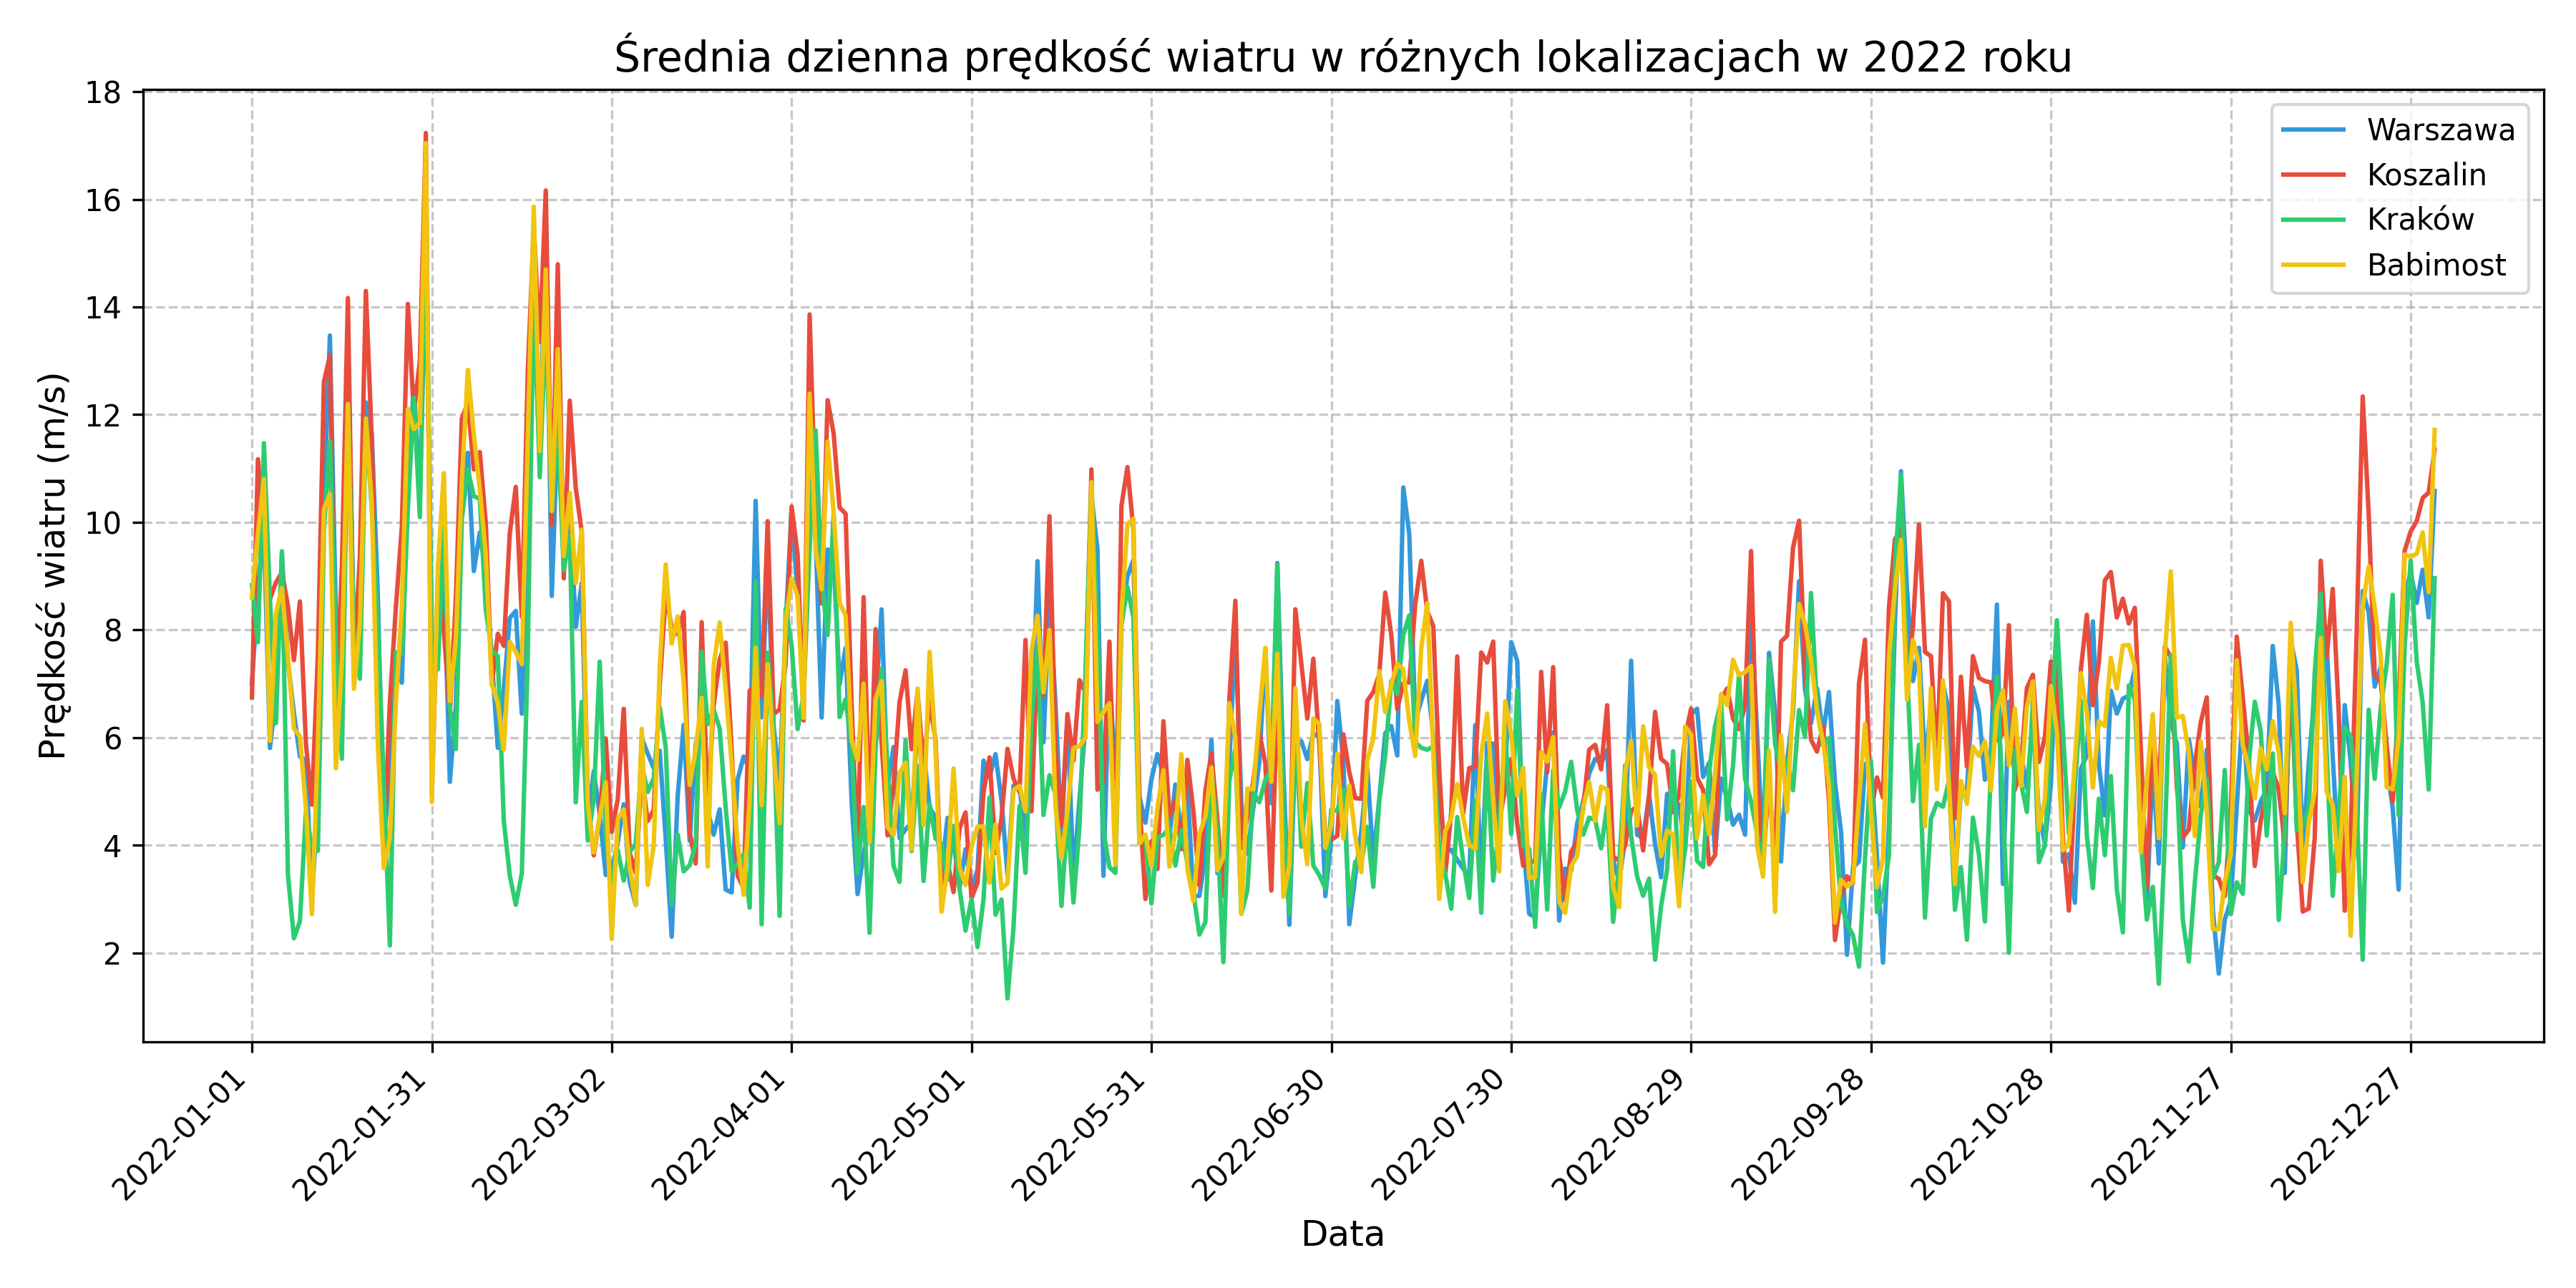
\includegraphics[width=\textwidth]{../plots/weather/wind_speed_time_series_2022.png}
    \caption{Zmienność prędkości wiatru w czasie (2022). Opracowanie własne na podstawie danych open-meteo.}
    \label{fig:wind-speed-time-series-2022}
\end{figure}

\begin{figure}[H]
    \centering
    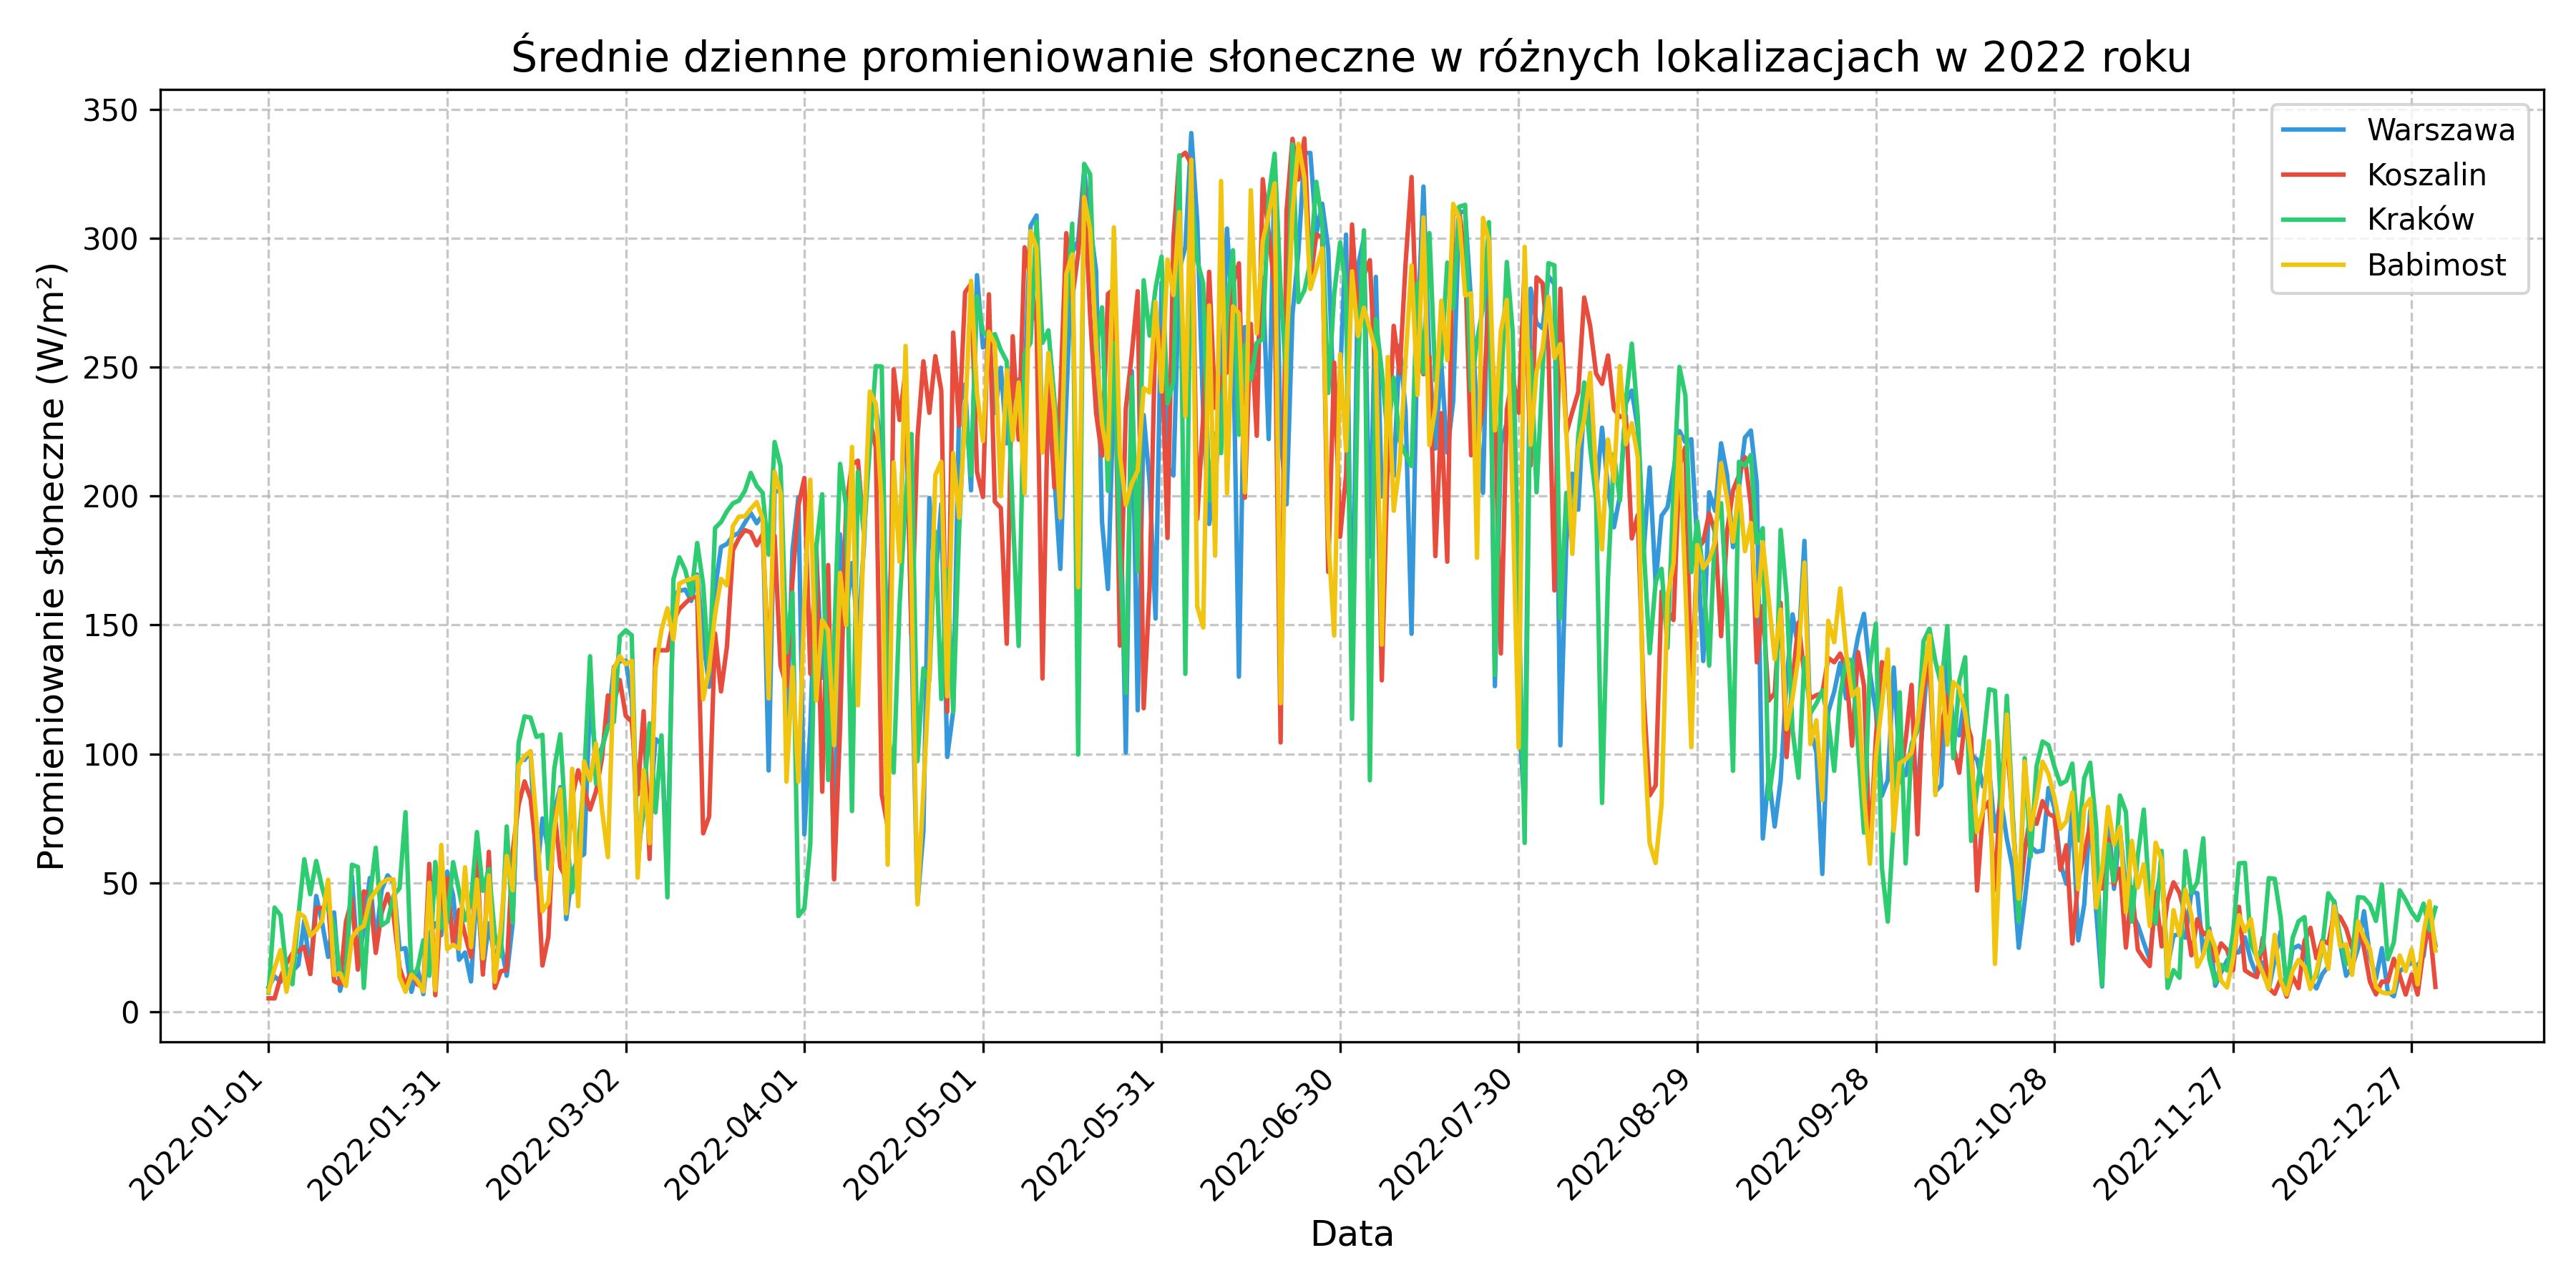
\includegraphics[width=\textwidth]{../plots/weather/solar_radiation_time_series_2022.png}
    \caption{Zmienność promieniowania słonecznego w czasie (2022). Opracowanie własne na podstawie danych open-meteo.}
    \label{fig:solar-radiation-time-series-2022}
\end{figure}

\begin{figure}[H]
    \centering
    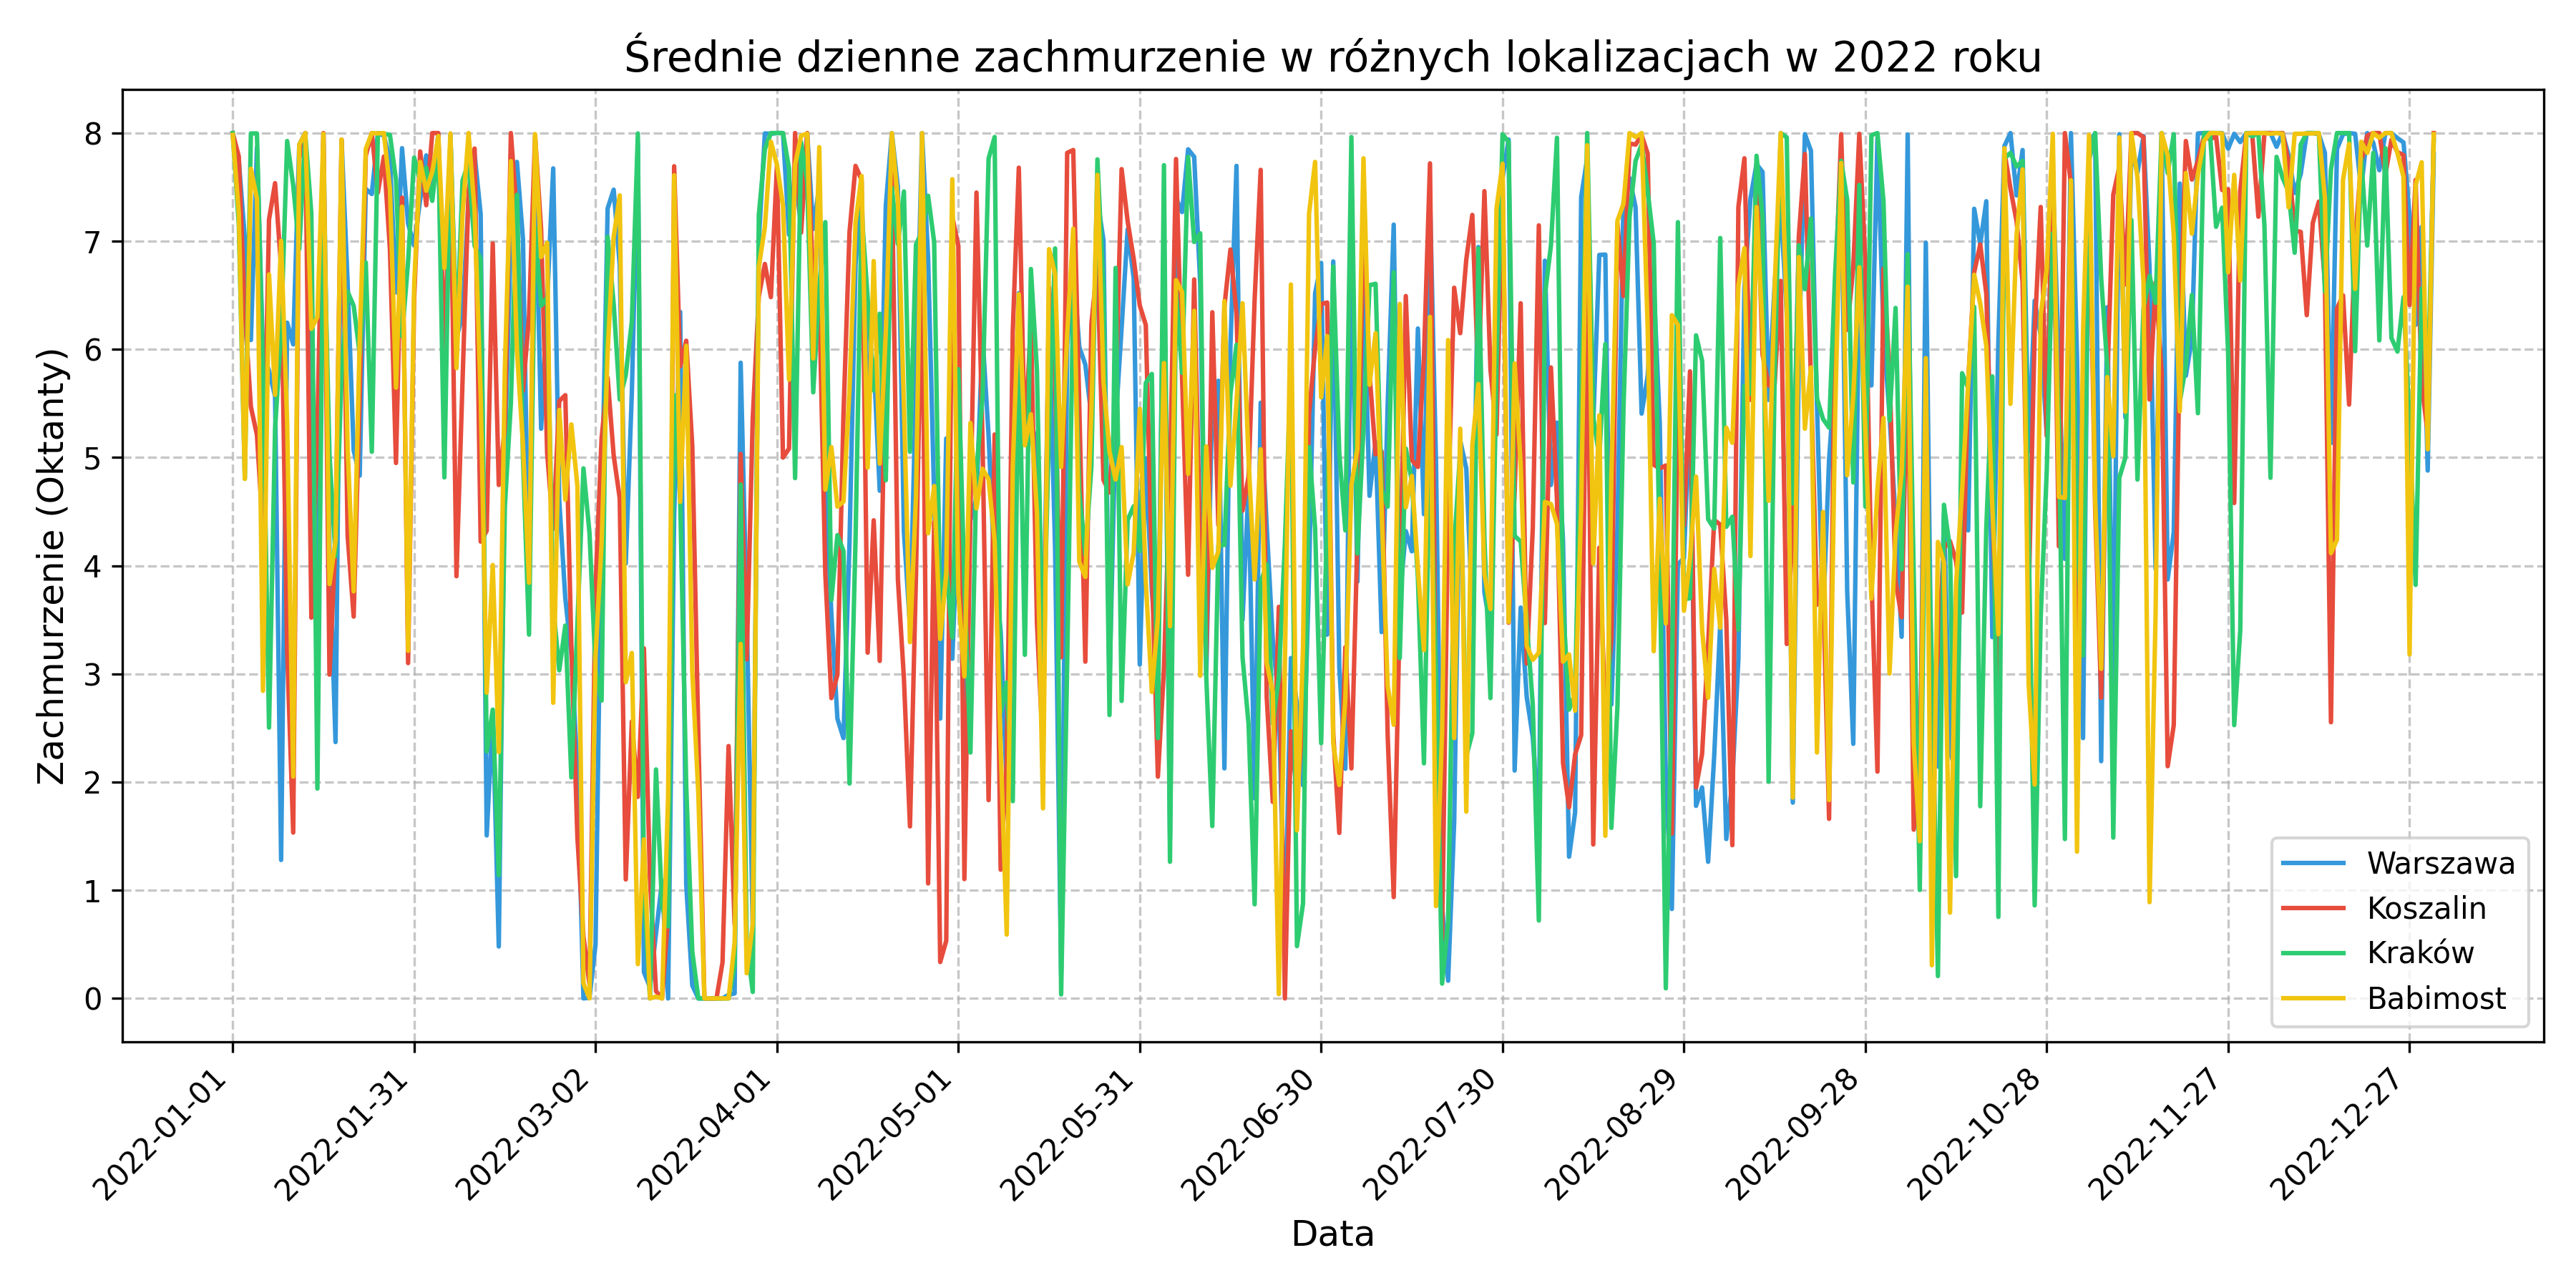
\includegraphics[width=\textwidth]{../plots/weather/cloud_cover_time_series_2022.png}
    \caption{Zmienność zachmurzenia w czasie (2022). Opracowanie własne na podstawie danych open-meteo.}
    \label{fig:cloud-cover-time-series-2022}
\end{figure}

Temperatura jest rzadko uwzględniana w modelach prognostycznych cen energii, ponieważ jej związek z produkcją energii nie jest bezpośredni. W kontekście Polski, gdzie znaczna część energii elektrycznej pochodzi z elektrowni węglowych, temperatura odgrywa jednak istotną rolę pośrednią, wpływając na zapotrzebowanie na energię, zwłaszcza w okresie sezonu grzewczego. Włączenie zmiennej do analizy może więc dostarczyć cennych informacji o sezonowych wzorcach konsumpcji i ich wpływie na dynamikę cen energii

\subsection{Produkcja energii z wybranych źródeł}
Zmienne dotyczące produkcji energii z różnych źródeł odgrywają kluczową rolę w analizie cen energii na RDN, ponieważ odzwierciedlają strukturę podaży energii w Polsce, która ma bezpośredni wpływ na dynamikę cen. W niniejszej pracy uwzględniono osiem zmiennych opisujących produkcję energii: 
\begin{itemize}
    \item \textbf{hard\_coal} - produkcja z węgla kamiennego (MWh),
    \item \textbf{coal\_derived} - produkcja z paliw pochodnych węgla (MWh),
    \item \textbf{lignite} - produkcja z węgla brunatnego (MWh),
    \item \textbf{gas} - produkcja z gazu ziemnego (MWh),
    \item \textbf{oil} - produkcja z ropy naftowej lub jej pochodnych (MWh),
    \item \textbf{biomass} - produkcja z biomasy (MWh),
    \item \textbf{wind} - produkcja z elektrowni wiatrowych lądowych (MWh),
    \item \textbf{solar} - produkcja z paneli fotowoltaicznych (MWh).
\end{itemize}

Dane te pochodzą z Polskich Sieci Elektroenergetycznych (PSE) \cite{PSEOLD} i zostały dopasowane do godzinowego formatu danych RDN, co pozwoliło na ich integrację z pozostałymi zmiennymi. 
\begin{figure}[H]
    \centering
    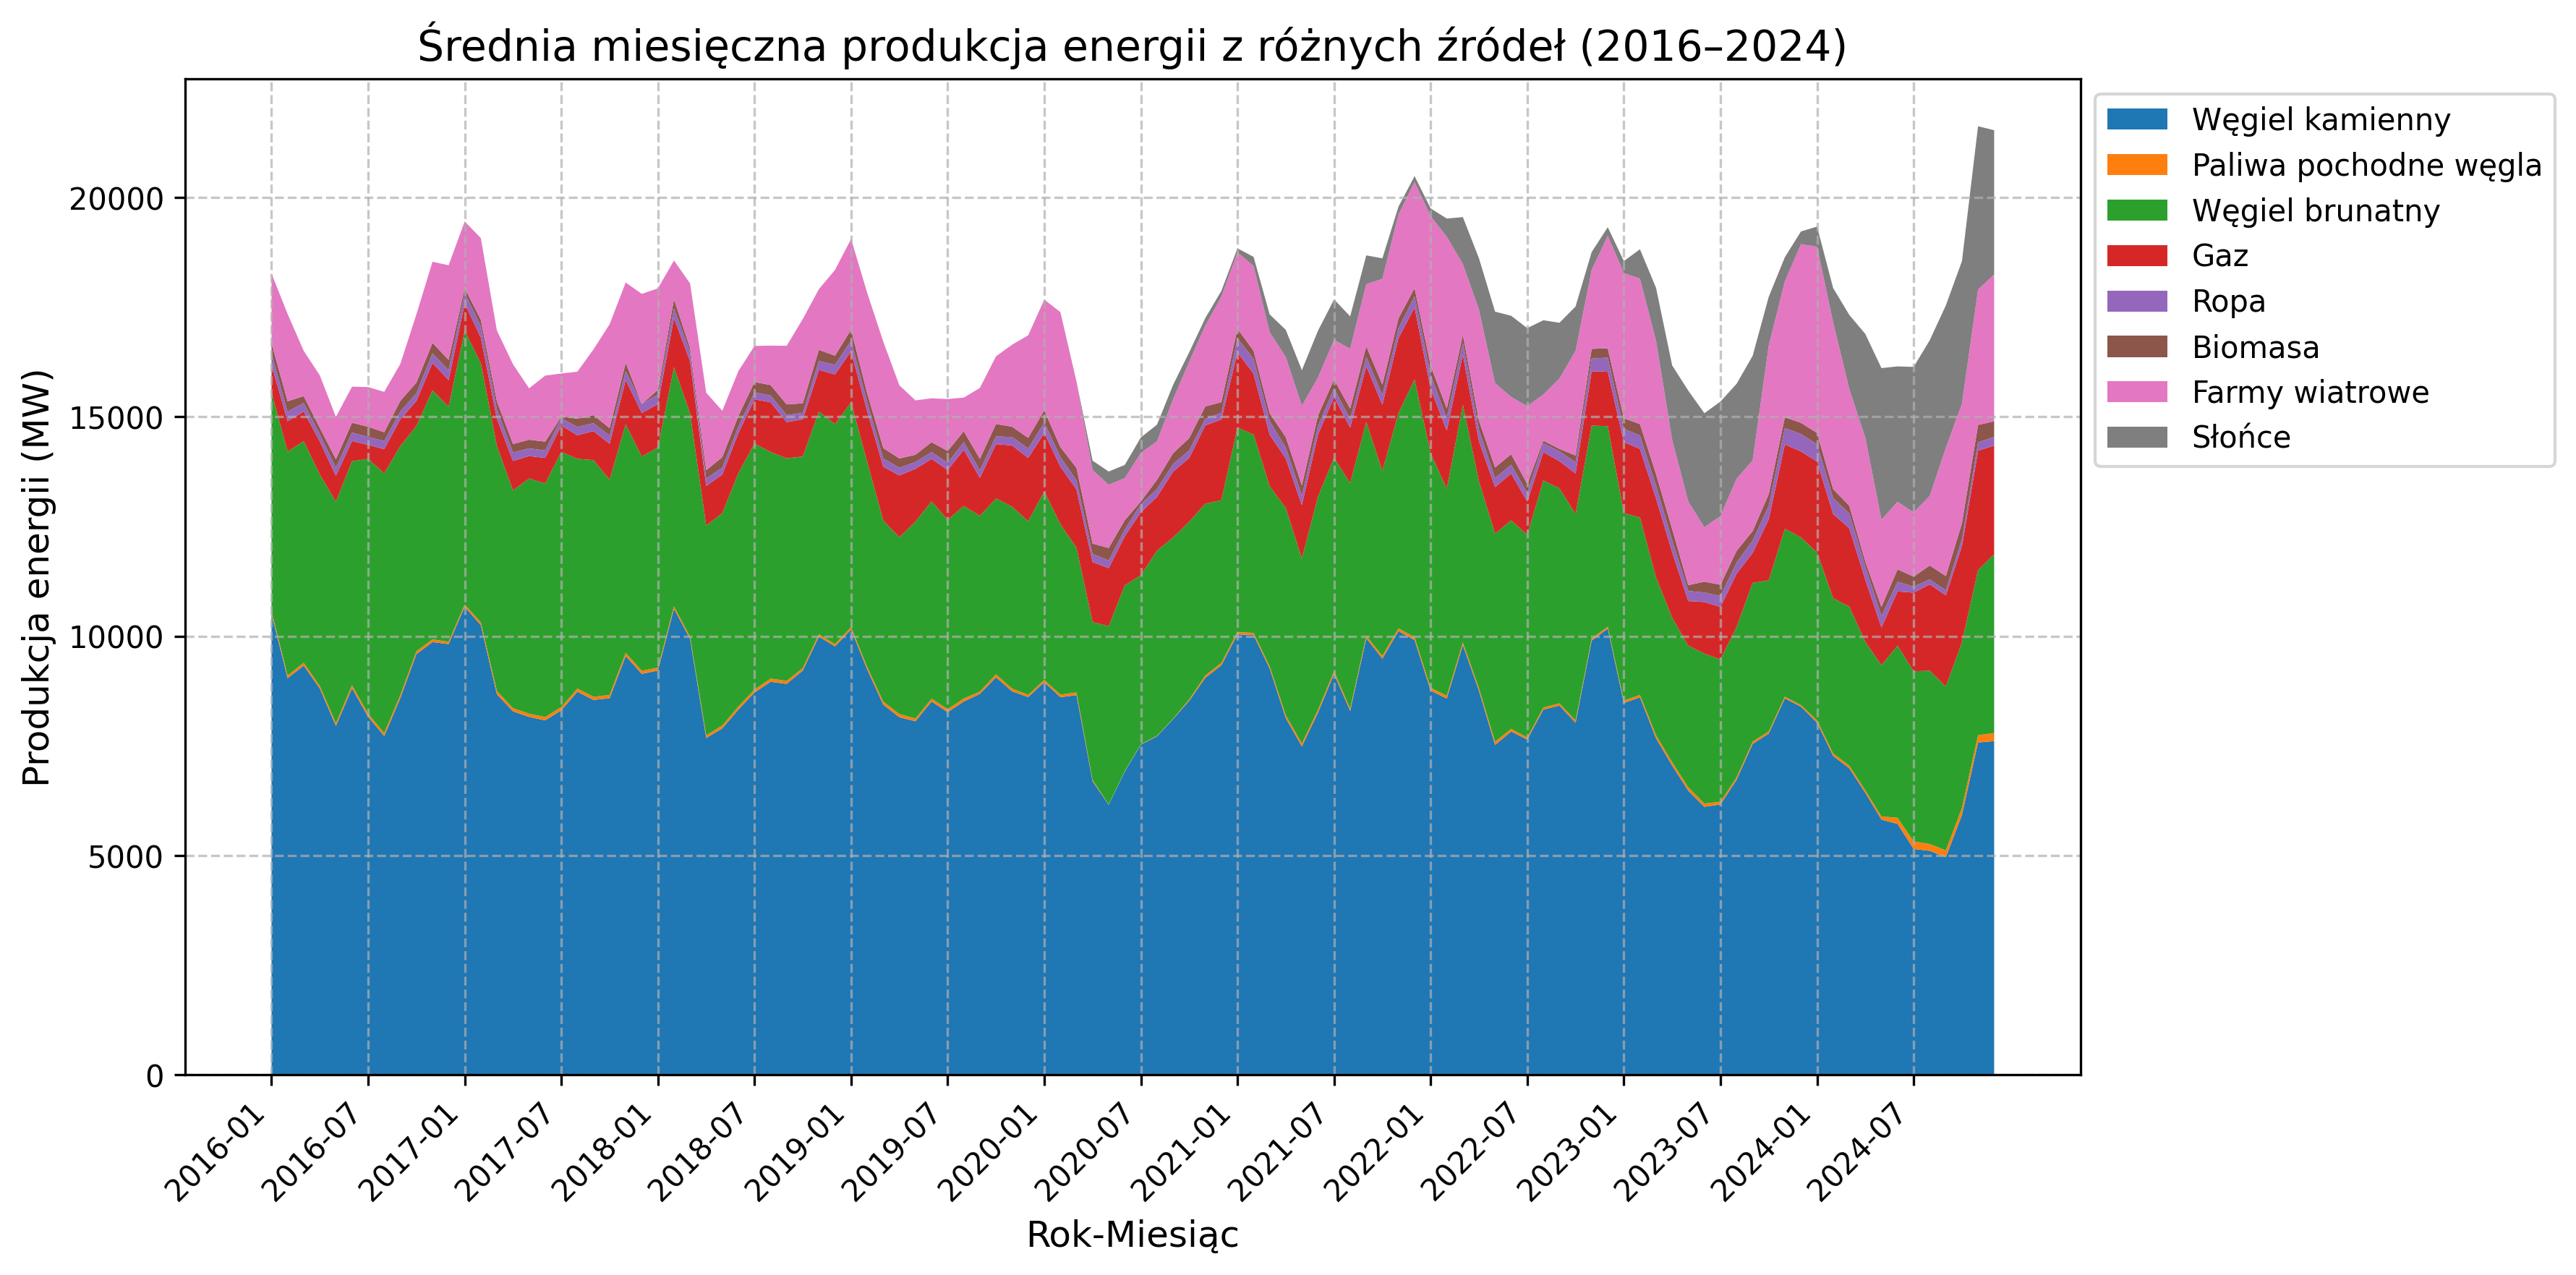
\includegraphics[width=1.0\textwidth]{../plots/energy/energy_production_time_series_full.png}
    \caption{Zmienność produkcji energii z różnych źródeł w czasie}
    \label{fig:energy-production-time-series-full}
\end{figure}

Wykres powyżej przedstawia średnią miesięczną produkcję energii z różnych źródeł w Polsce w latach 2016-2023, co jest istotne w kontekście prognozowania cen energii na RDN. Wykres obszarowy ukazuje dominację węgla kamiennego i węgla brunatnego, które do tej pory odpowiadają za większość produkcji energii elektrycznej. Biomasa oraz paliwa pochodne węgla stanowią znikomą część podaży i mogą być pominięte dla redukcji ilości zmiennych. Produkcja za pomocą gazu i ropy stale posiada niewielką, ale istotną część produkcji energii. Warto zauważyć, że produkcja z OZE, szczególnie ze słońca znacząco rośnie w ostatnich latach, co może mieć istotny wpływ na ceny energii i umiejętność jej prognozowania. Do poprzednio omówionych zmiennych dodano również zmienną \texttt{non\_emissive\_sources\_percentage}, która reprezentuje procentowy udział energii produkowanej z OZE w całkowitej produkcji energii elektrycznej w Polsce. Warto zaznaczyć, że średnia wartość produkcji energii z OZE w całym zakresie danych wynosi 14\%, gdyż średnia wartość w 2023 wynosi już 23\%. Wskazuje to wyraźną dynamikę wzrostu udziału OZE w systemie energetycznym kraju.
\begin{figure}[H]
    \centering
    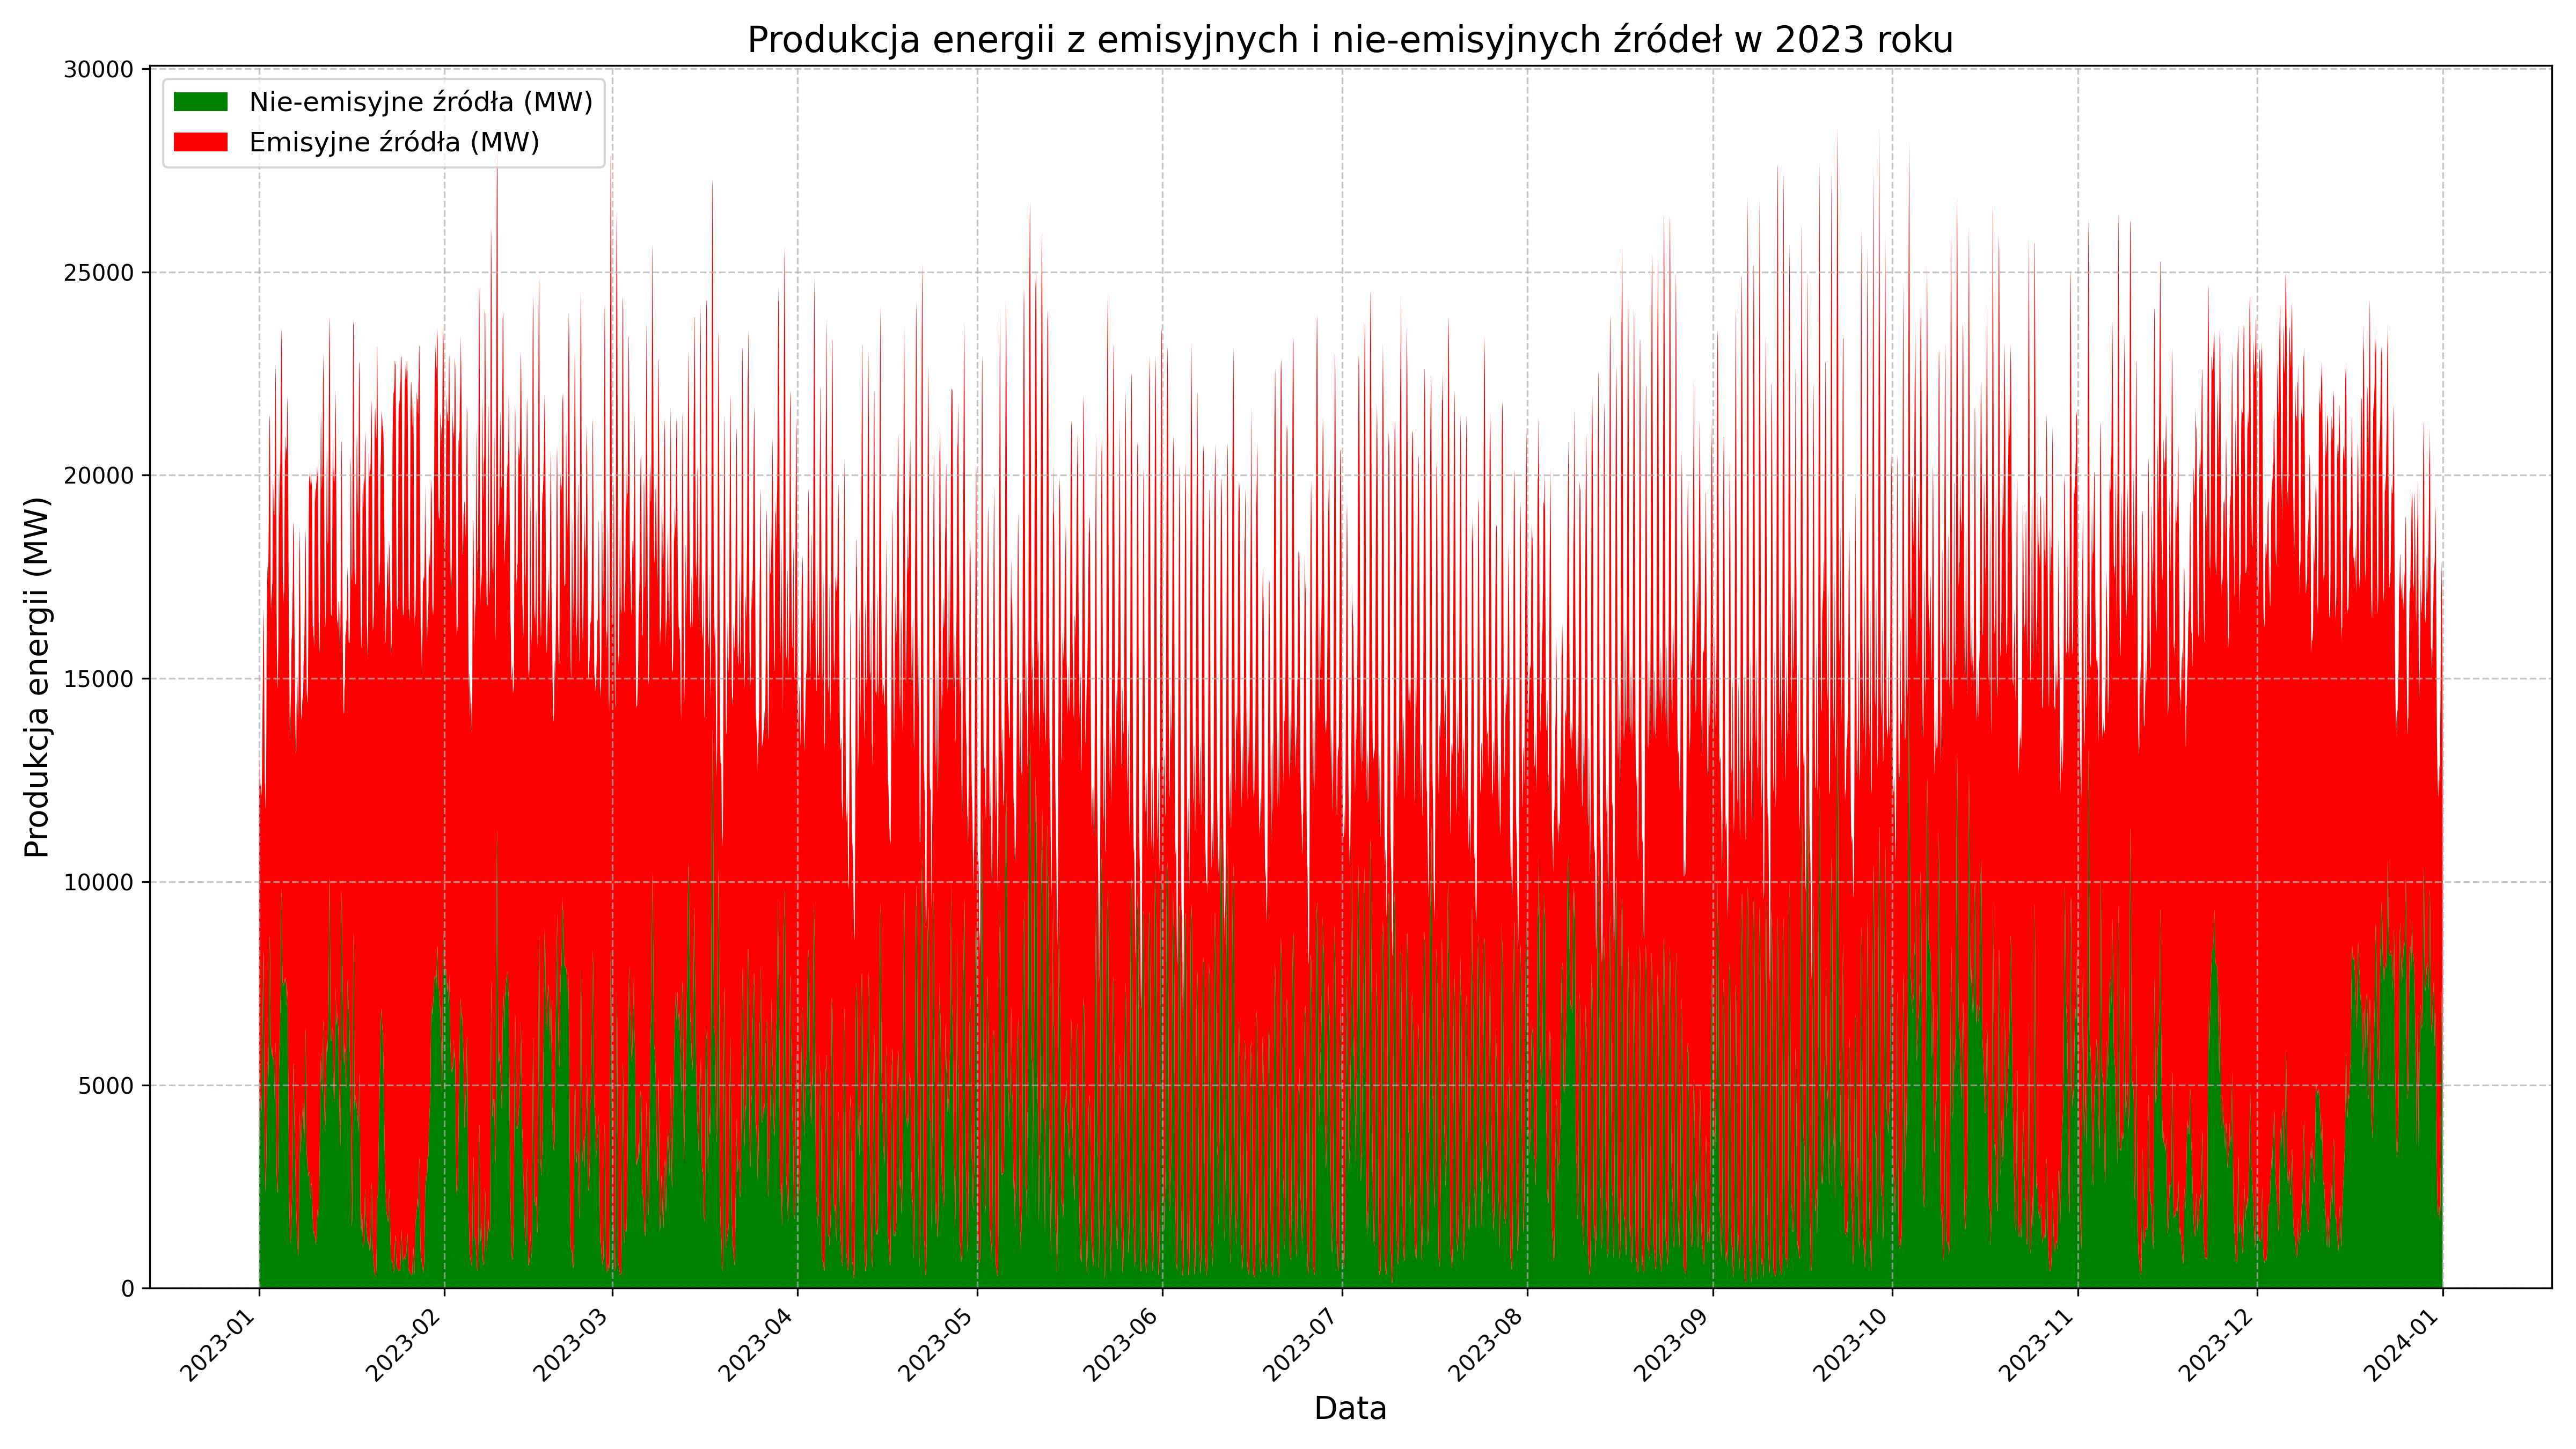
\includegraphics[width=\textwidth]{../plots/energy/emission_vs_non_emission_2023_high_res.png}
    \caption{Porównanie produkcji energii z emisyjnych i bezemisyjnych źródeł w 2023 roku. Opracowanie własne na podstawie danych PSE.}
    \label{fig:emission-vs-non-emission-2023}
\end{figure}
W niektórych godzinach udział OZE w produkcji energii może przekraczać udział źródeł emisyjnych, co zwykle prowadzi do spadku cen. Warto również zauważyć, że produkcja z węgla kamiennego i brunatnego jest bardziej stabilna i przewidywalna niż produkcja z OZE, co wpływa na dokładność prognoz. W związku z tym, zmienne dotyczące produkcji energii z różnych źródeł są istotnym elementem modelowania cen energii.

\subsection{Handel energią z państwami sąsiednimi}
\label{subsec:trade}
Zmienne dotyczące wymiany energii z innymi krajami są kolejnym istotnym elementem analizy cen energii na Rynku Dnia Następnego, ponieważ pozwalają na uwzględnienie wpływu handlu międzynarodowego na ceny energii w Polsce. W niniejszej pracy uwzględnione zostały bilanse handlu energią z Państwami sąsiednimi, z którymi Polska ma połączenia transgraniczne. Są to Państwa takie jak:
\begin{itemize}
    \item Niemcy (DE),
    \item Czechy (CZ),
    \item Słowacja (SK),
    \item Litwa (LT),
    \item Szwecja (SE),
    \item Ukraina (UA).
\end{itemize}

Dane dotyczące wymiany energii z tymi krajami pochodzą z Polskich Sieci Elektroenergetycznych i są dostępne w granulacji godzinowej. Warto zauważyć, że Polska jest jednym z kluczowych graczy na rynku energii w Europie Środkowo-Wschodniej, co sprawia, że wymiana energii zwykle występuje z każdym krajem w każdej godzinie czasu rzeczywistego. W okresach wysokiego zapotrzebowania na energię lub w sytuacjach poważnych awarii, Polska sięga po energię z innych krajów, co prowadzi do wzrostu cen. Z drugiej strony, w okresach niskiego zapotrzebowania, Polska może eksportować, czyli sprzedawać nadwyżki energii, w momentach spadków cen. Prawdopodobnie, taki aktywny handel może również wynikać z różnic cenowych pomiędzy krajami. Poniżej przedstawiam tabele wymiany energii z sąsiadami w latach 2016-2023.

\begin{table}[H]
    \centering
    \resizebox{\textwidth}{!}{%
    \begin{tabular}{|c|r|r|r|r|r|r|}
    \hline
    \textbf{Rok} & \textbf{Niemcy (MW)} & \textbf{Czechy (MW)} & \textbf{Litwa (MW)} & \textbf{Słowacja (MW)} & \textbf{Szwecja (MW)} & \textbf{Ukraina (MW)} \\ \hline
    2016 & 994.26  & -761.81 & 68.21   & -475.47 & 294.36  & 108.99  \\ \hline
    2017 & 836.24  & -612.73 & 119.92  & -499.21 & 340.96  & 102.45  \\ \hline
    2018 & 803.00  & -373.78 & 102.53  & -366.14 & 310.83  & 160.96  \\ \hline
    2019 & 1149.22 & -312.31 & 216.38  & -367.32 & 329.80  & 157.17  \\ \hline
    2020 & 1275.75 & -264.90 & 201.93  & -348.95 & 428.81  & 167.98  \\ \hline
    2021 & 957.79  & -901.92 & 110.04  & -519.59 & 364.69  & 93.55   \\ \hline
    2022 & 918.62  & -1000.89 & 86.53  & -684.25 & 429.17  & 126.95  \\ \hline
    2023 & 851.27  & -526.46 & 58.40   & -382.18 & 431.60  & 5.76    \\ \hline
    \end{tabular}%
    }
    \caption{Średni bilans wymiany energii z sąsiadami w latach 2016-2023. Opracowanie własne na podstawie danych PSE.}
    \label{tab:energy-trade-balance}
\end{table}

Wartości te są średniogodzinowymi bilansami wymiany energii z sąsiadami w latach 2016-2023. Wartości dodatnie oznaczają eksport energii, a wartości ujemne import energii. Polska ma dodatni bilans wymiany energii z Niemcami, co oznacza, że regularnie eksportuje energię do Niemiec. Największe ujemne bilanse Polska posiada z Czechami, prawdopodobnie spowodowane jest to funkcjonującymi w Czechami elektrowniami atomowymi. Przepływy transgraniczne są warte uwagi i uwględnienia w zbiorze.

Dodatkowo, w analizie uwzględniono dane cenowe z rynków sąsiednich, które odzwierciedlają koszty energii w tych krajach i mogą wpływać na decyzje o imporcie lub eksporcie. Zebrane dane cenowe obejmują cztery obszary: Czechy (CZ), Słowację (SK), Litwę (LT) oraz Szwecję (SE4). Szwedzki rynek energii elektrycznej jest podzielony na cztery obszary i właśnie ten ostatni - południowy jest połączony z systemem Polskim. Dane cenowe zostały pobrane ze strony transparency entsoe \cite{transparency_entso}, będącej oficjalnym źródłem danych ENTSO-E, czyli Europejskiej Sieci Operatorów Systemów Przesyłowych Energii Elektrycznej. Dane dostępne są w rozdzielczości godzinowej podobnie do Polskiego rynku. \newline Dane cenowe z rynku ukraińskiego (UA) są dostępne dopiero od grudnia 2020 roku, co uniemożliwiło ich uwzględnienie w analizie dla całego okresu. Podobnie, dane z rynku niemieckiego (DE) są dostępne dopiero od października 2018 roku, dlatego również zostały pominięte. Brak tych danych wynika z ograniczeń dostępności historycznych informacji na wspomnianej platformie.

Wszystkie dane cenowe z rynków sąsiednich, pierwotnie wyrażone w euro na megawatogodzinę, zostały przekonwertowane na PLN/MWh zgodnie z kursem średnim Narodowego Banku Polskiego dla odpowiednich dat. Przeliczenie to zapewniło ujednolicenie jednostek walutowych z innymi zmiennymi w zbiorze, takimi jak zmienna zależna. Włączenie tych cen do modelu pozwala na analizę wpływu różnic cenowych między krajami na handel energią oraz na dynamikę cen w Polsce, co jest szczególnie istotne w okresach zmiennej dostępności energii odnawialnej lub w sytuacjach kryzysowych. Poniżej załączam tabele statystyk cenowych z rynków sąsiednich w latach 2016-2023 podobnie do tych przedstawionych dla zmiennej zależnej \ref{tab:fixing-i-price-stats}.

\begin{table}[H]
    \centering
    \resizebox{\textwidth}{!}{%
    \begin{tabular}{|l|r|r|r|r|}
    \hline
    \textbf{Statystyka} & \textbf{Szwecja (SE4) } & \textbf{Słowacja (SK)} & \textbf{Czechy (CZ)} & \textbf{Litwa (LT)} \\ \hline
    Średnia & 265.92 PLN/MWh & 380.30 PLN/MWh & 361.74 PLN/MWh & 349.51 PLN/MWh \\ \hline
    Odchylenie std. & 332.26 PLN/MWh & 453.45 PLN/MWh & 428.63 PLN/MWh & 418.34 PLN/MWh \\ \hline
    Minimum & -267.23 PLN/MWh & -293.49 PLN/MWh & -310.33 PLN/MWh & -251.70 PLN/MWh \\ \hline
    25\% (Q1) & 115.20 PLN/MWh & 141.34 PLN/MWh & 138.38 PLN/MWh & 141.41 PLN/MWh \\ \hline
    Mediana & 165.57 PLN/MWh & 210.72 PLN/MWh & 201.64 PLN/MWh & 202.91 PLN/MWh \\ \hline
    75\% (Q3) & 260.83 PLN/MWh & 420.55 PLN/MWh & 405.60 PLN/MWh & 373.50 PLN/MWh \\ \hline
    Maksimum & 3786.10 PLN/MWh & 4260.61 PLN/MWh & 4139.78 PLN/MWh & 9991.76 PLN/MWh \\ \hline
    \end{tabular}%
    }
    \caption{Statystyki cen energii (PLN/MWh) na rynkach sąsiednich w okresie 2016-2023. Opracowanie własne na podstawie danych ENTSO-E.}
    \label{tab:market-price-statistics-full-period}
\end{table}

Statystyki pokazują, że ceny energii na rynkach sąsiednich są bardziej zmienne niż ceny na RDN, co może być wynikiem różnic w strukturze rynku, dostępności źródeł energii oraz polityki energetycznej w poszczególnych krajach oraz waluty euro, w której są wyrażone. Wartości minimalne i maksymalne wskazują na występowanie ekstremalnych zdarzeń cenowych, które mogą mieć istotny wpływ na handel energią oraz na ceny w Polsce. Na przykład, w sierpniu 2022 roku ceny energii na Litwie osiągały rekordowy poziom 9991.76 PLN/MWh.

\subsection{Ceny paliw kopalnych i emisji CO2}
\label{subsec:prices}

Zmienne dotyczące cen paliw kopalnych oraz emisji CO$_2$ odgrywają kluczową rolę w analizie cen energii na RDN, ponieważ koszty paliw i emisji mają bezpośredni wpływ na ceny energii elektrycznej w Polsce, gdzie dominującym źródłem energii jest węgiel. W niniejszej pracy uwzględniono cztery zmienne, które zostały opisane w Tabeli~\ref{tab:fuel_variables}.

\begin{table}[H]
    \centering
    \begin{tabular}{|l|l|l|l|}
    \hline
    \textbf{Nazwa zmiennej} & \textbf{Opis} & \textbf{Źródło danych} & \textbf{Rozdzielczość} \\ \hline
    \texttt{gas\_price}     & Cena gazu ziemnego (PLN/MWh) & instrat \cite{INSTRAT_ENERGY} & Dzienna \\ \hline
    \texttt{coal\_price}    & Cena węgla kamiennego (PLN/GJ) & instrat \cite{INSTRAT_ENERGY} & miesięczna \\ \hline
    \texttt{co2\_price}     & Cena uprawnień do emisji CO$_2$ (PLN/tCO$_2$) & instrat \cite{INSTRAT_ENERGY} & tygodniowa \\ \hline
    \texttt{brent\_price}   & Cena ropy Brent Europe (PLN/bar) & EIA \cite{EIA} & Dzienna \\ \hline
    \end{tabular}
    \caption{Opis zmiennych dotyczących cen paliw kopalnych i emisji CO$_2$.}
    \label{tab:fuel_variables}
\end{table}

Dane te zostały dopasowane do godzinowego formatu danych RDN, w taki sposób, że w dniach pracy giełdy i znanych cen paliw, cena stale jest przypisana do godzin, a w dniach wolnych od pracy lub bez znanych cen, wartości są interpolowane. 

Ceny paliw kopalnych i emisji CO$_2$ są istotne w kontekście prognozowania cen energii, ponieważ wpływają na koszty produkcji energii w elektrowniach konwencjonalnych, które dominują w polskim miksie energetycznym. Na przykład, wzrost ceny węgla (\texttt{coal\_price}) lub uprawnień do emisji CO$_2$ (\texttt{co2\_price}) zwiększa koszty produkcji energii w elektrowniach węglowych. Cena gazu (\texttt{gas\_price}) jest kluczowa dla elektrowni gazowych, które pełnią rolę bilansującą w systemie. Cena ropy Brent (\texttt{brent\_price}) ma mniejszy bezpośredni wpływ na produkcję energii w Polsce, ale jest istotna w kontekście globalnych trendów cen paliw i skorelowana z innymi cenami surowców energetycznych.

Aby zilustrować dynamikę tych zmiennych, na rysunku poniżej przedstawiono zmiany cen paliw kopalnych i emisji CO$_2$ w latach 2016-2023 w ujęciu miesięcznym. Dla lepszego przedstawienia danych użyłem skali logarytmicznej.

\begin{figure}[h]
    \centering
    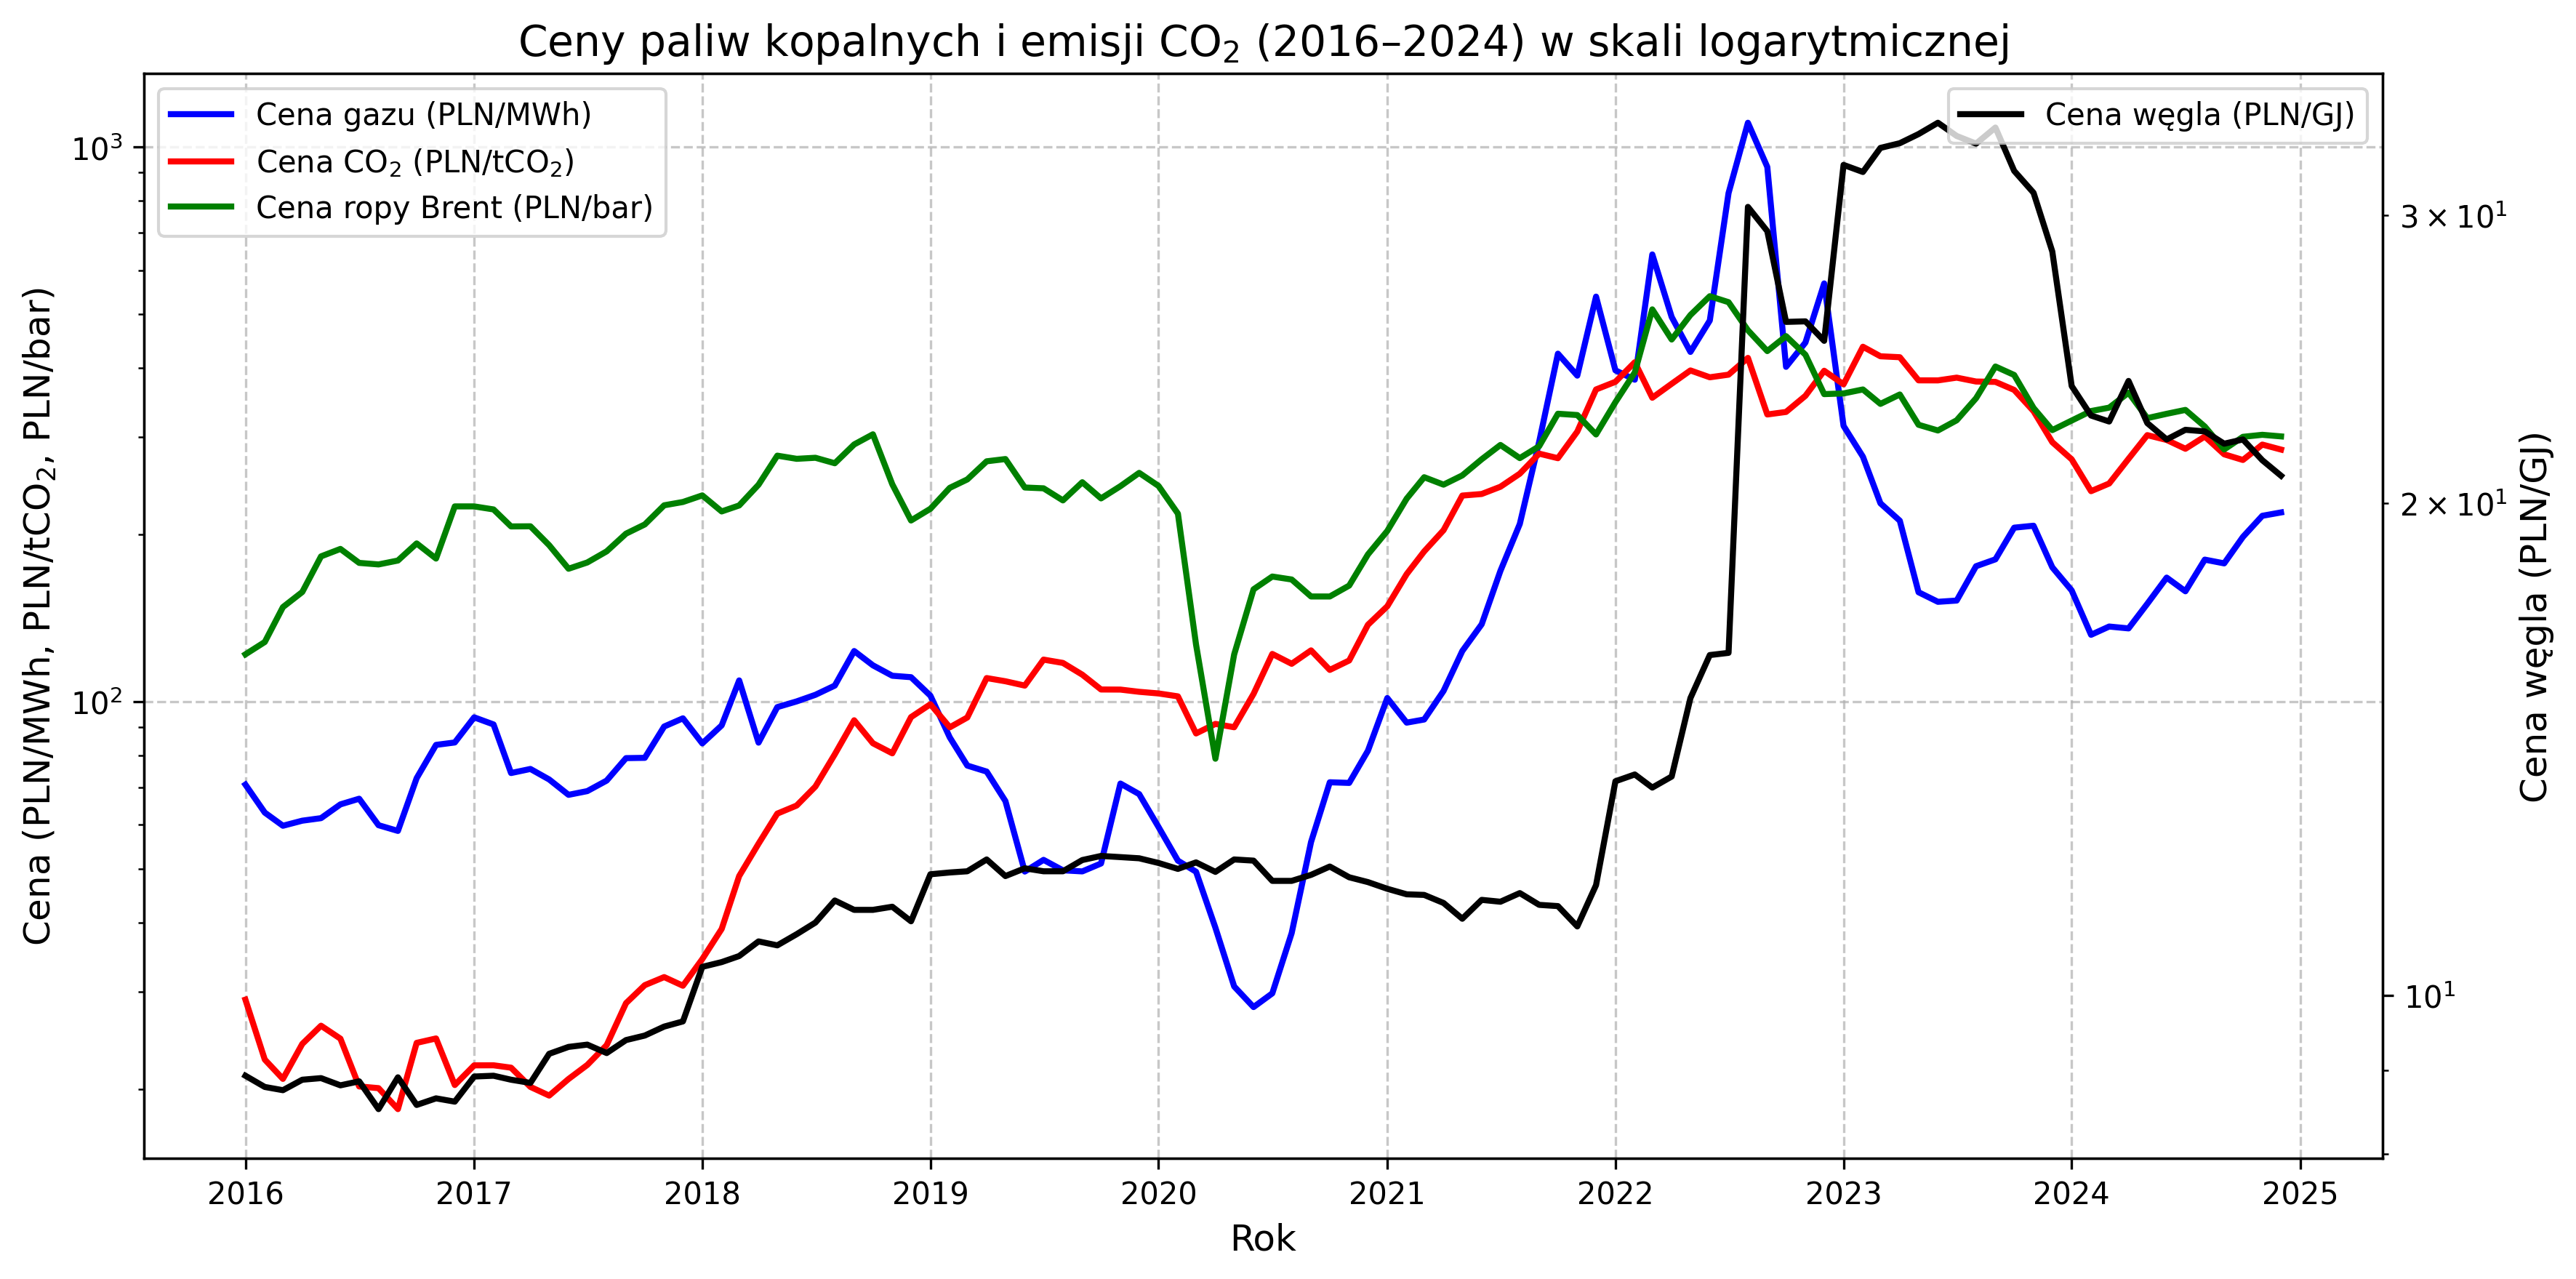
\includegraphics[width=0.9\textwidth]{../plots/fuels/fuel_prices_2016_2024.png}
    \caption{Ceny paliw kopalnych i emisji CO$_2$ w latach w ujęciu miesięcznym. Źródło: Opracowanie własne na podstawie danych rynkowych.}
    \label{fig:fuel_prices}
\end{figure}

Ceny paliw kopalnych w okresie wysokiej zmienności szybko rosną, co jest jedną z przyczyn rosnących cen energii. Największy wzrost ma cena gazu, która od rozpoczęcia konfliktu zbrojnego wzrosła ponad 10-krotnie w ciągu roku. 

\subsection{Straty mocy w systemie elektroenergetycznym}
\label{subsec:losses}

Zmienne dotyczące strat mocy w systemie elektroenergetycznym odgrywają istotną rolę w analizie cen energii na Rynku Dnia Następnego (RDN), ponieważ wpływają na dostępność energii w systemie oraz koszty jej przesyłu i dystrybucji. W niniejszej pracy uwzględniono następujące dane zbierane przez systemy PSE: \texttt{power\_loss} (utrata mocy w wyniku awarii w MW) oraz \texttt{network\_loss} (utrata mocy w sieci w MW). Dane te są dostępne w rozdzielczości godzinowej i pochodzą z Polskich Sieci Elektroenergetycznych \cite{PSEOLD}.

Aby zilustrować dynamikę tych zmiennych, na rysunku~\ref{fig:power_losses} przedstawiono zmiany strat mocy w wyniku awarii (\texttt{power\_loss}) oraz strat mocy w sieci (\texttt{network\_loss}) w latach 2016-2023 w ujęciu miesięcznym.

\begin{figure}[h]
    \centering
    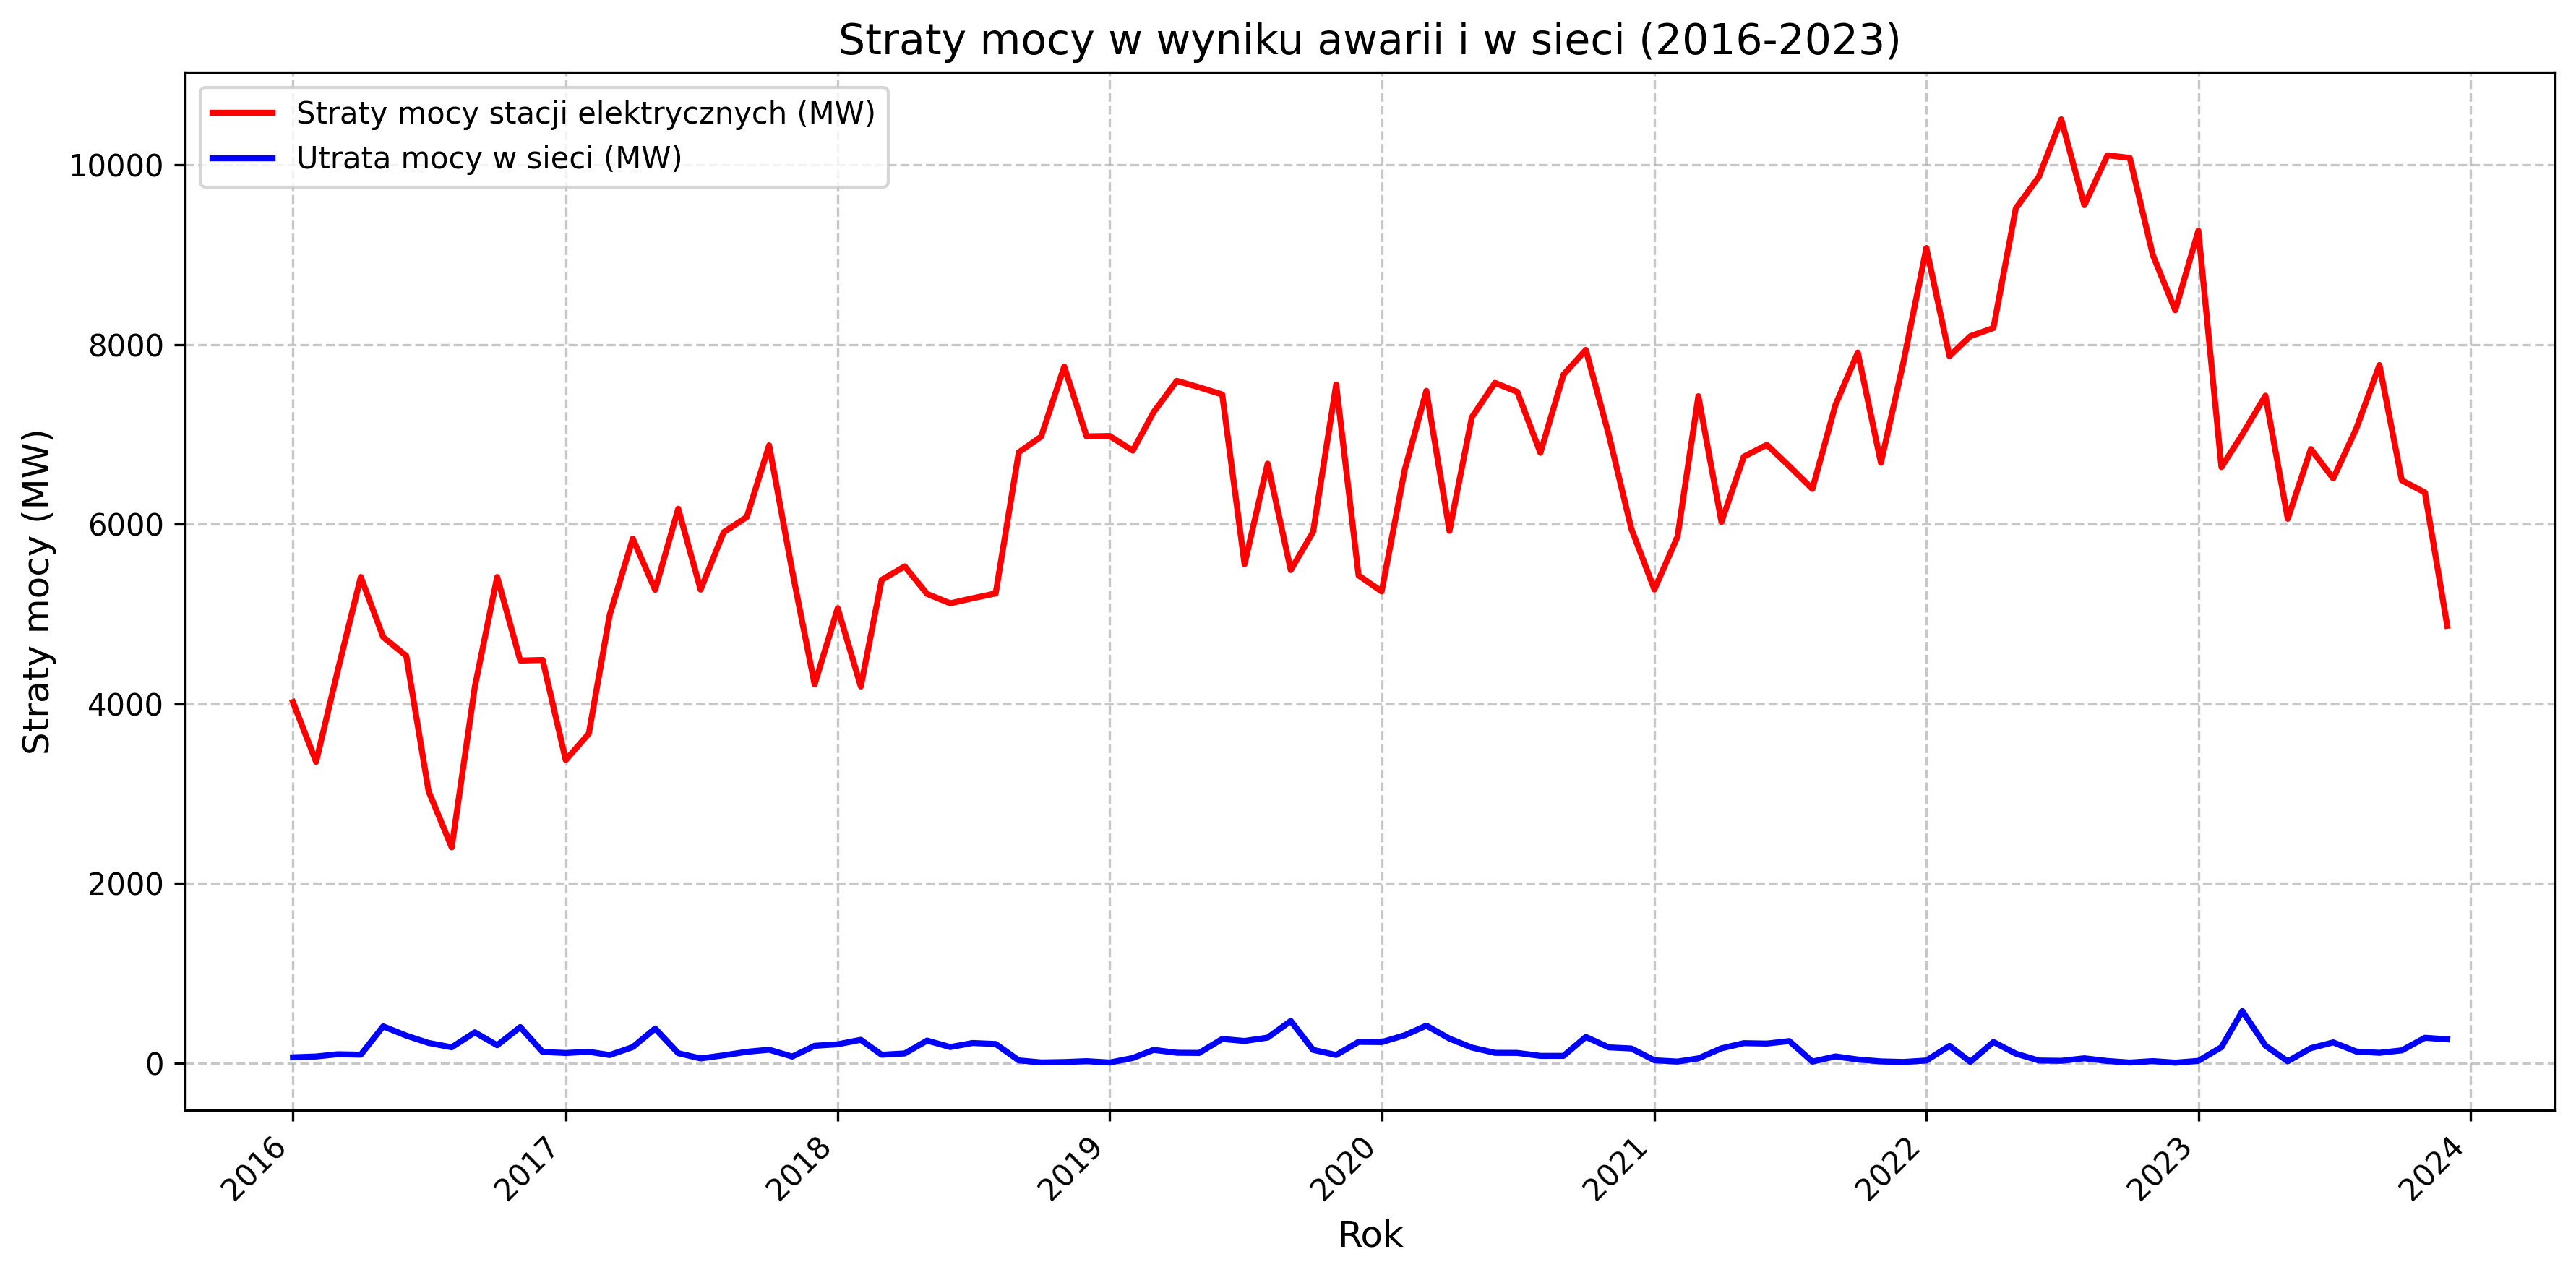
\includegraphics[width=1.0\textwidth]{../plots/losses/power_losses.png}
    \caption{Straty mocy w wyniku awarii i w sieci w ujęciu miesięcznym. Źródło: Opracowanie własne na podstawie danych z PSE.}
    \label{fig:power_losses}
\end{figure}

Analiza rysunku~\ref{fig:power_losses} ujawnia wyraźne różnice w dynamice obu zmiennych. Straty mocy w wyniku awarii (\texttt{power\_loss}, czerwona linia) wykazują znaczną zmienność w czasie, osiągając wartości od około 2 MW do szczytowych wartości przekraczających 10 000 MW. Największe szczyty można obserwować w roku 2022, co może być powiązane z kryzysem energetycznym oraz zwiększonym zapotrzebowaniem na energię w Europie, prowadzącym do przeciążeń systemu.

Staty mocy w sieci (\texttt{network\_loss}, niebieska linia) są znacznie bardziej stabilne. Warto zauważyć, że w 54.09\% przypadków zmienna \texttt{network\_loss} przyjmuje wartość 0, co wskazuje na brak strat mocy w sieci w ponad połowie analizowanych godzin. Stabilność strat sieciowych wynika z ich zależności od fizycznych właściwości systemu przesyłowego, takich jak długość linii, opór elektryczny czy poziom obciążenia, które zmieniają się w sposób bardziej przewidywalny niż losowe awarie.

Porównanie obu zmiennych wskazuje, że straty w wyniku awarii mają większy wpływ na krótkoterminowe wahania dostępności energii w systemie, co może bezpośrednio przekładać się na wzrost cen na RDN w okresach wysokich strat. Uwzględnienie tych zmiennych w modelowaniu cen energii pozwala na lepsze zrozumienie wpływu czynników technicznych na dynamikę rynku.

\subsection{Zapotrzebowanie na energię i wolumen handlu}
\label{subsec:demand}

Kolejnymi z ważnych zmiennych są zapotrzebowanie na energię i wolumen handlu. Przedstawiają one popyt na rynku, przez co można je określić podstawowymi czynnikami kształtującym ceny. W niniejszej pracy uwzględniono następujące zmienne: \texttt{load} (zapotrzebowanie na energię w MWh) oraz \texttt{trade\_volume} (wolumen handlu w MWh). Obie zmienne pochodzą z Polskich Sieci Elektroenergetycznych (PSE) i są dostępne w granulacji godzinowej.

Poniżej na wspólnym wykresie przedstawię różnice pomiędzy zapotrzebowaniem a wolumenem handlu.

\begin{figure}[H]
    \centering
    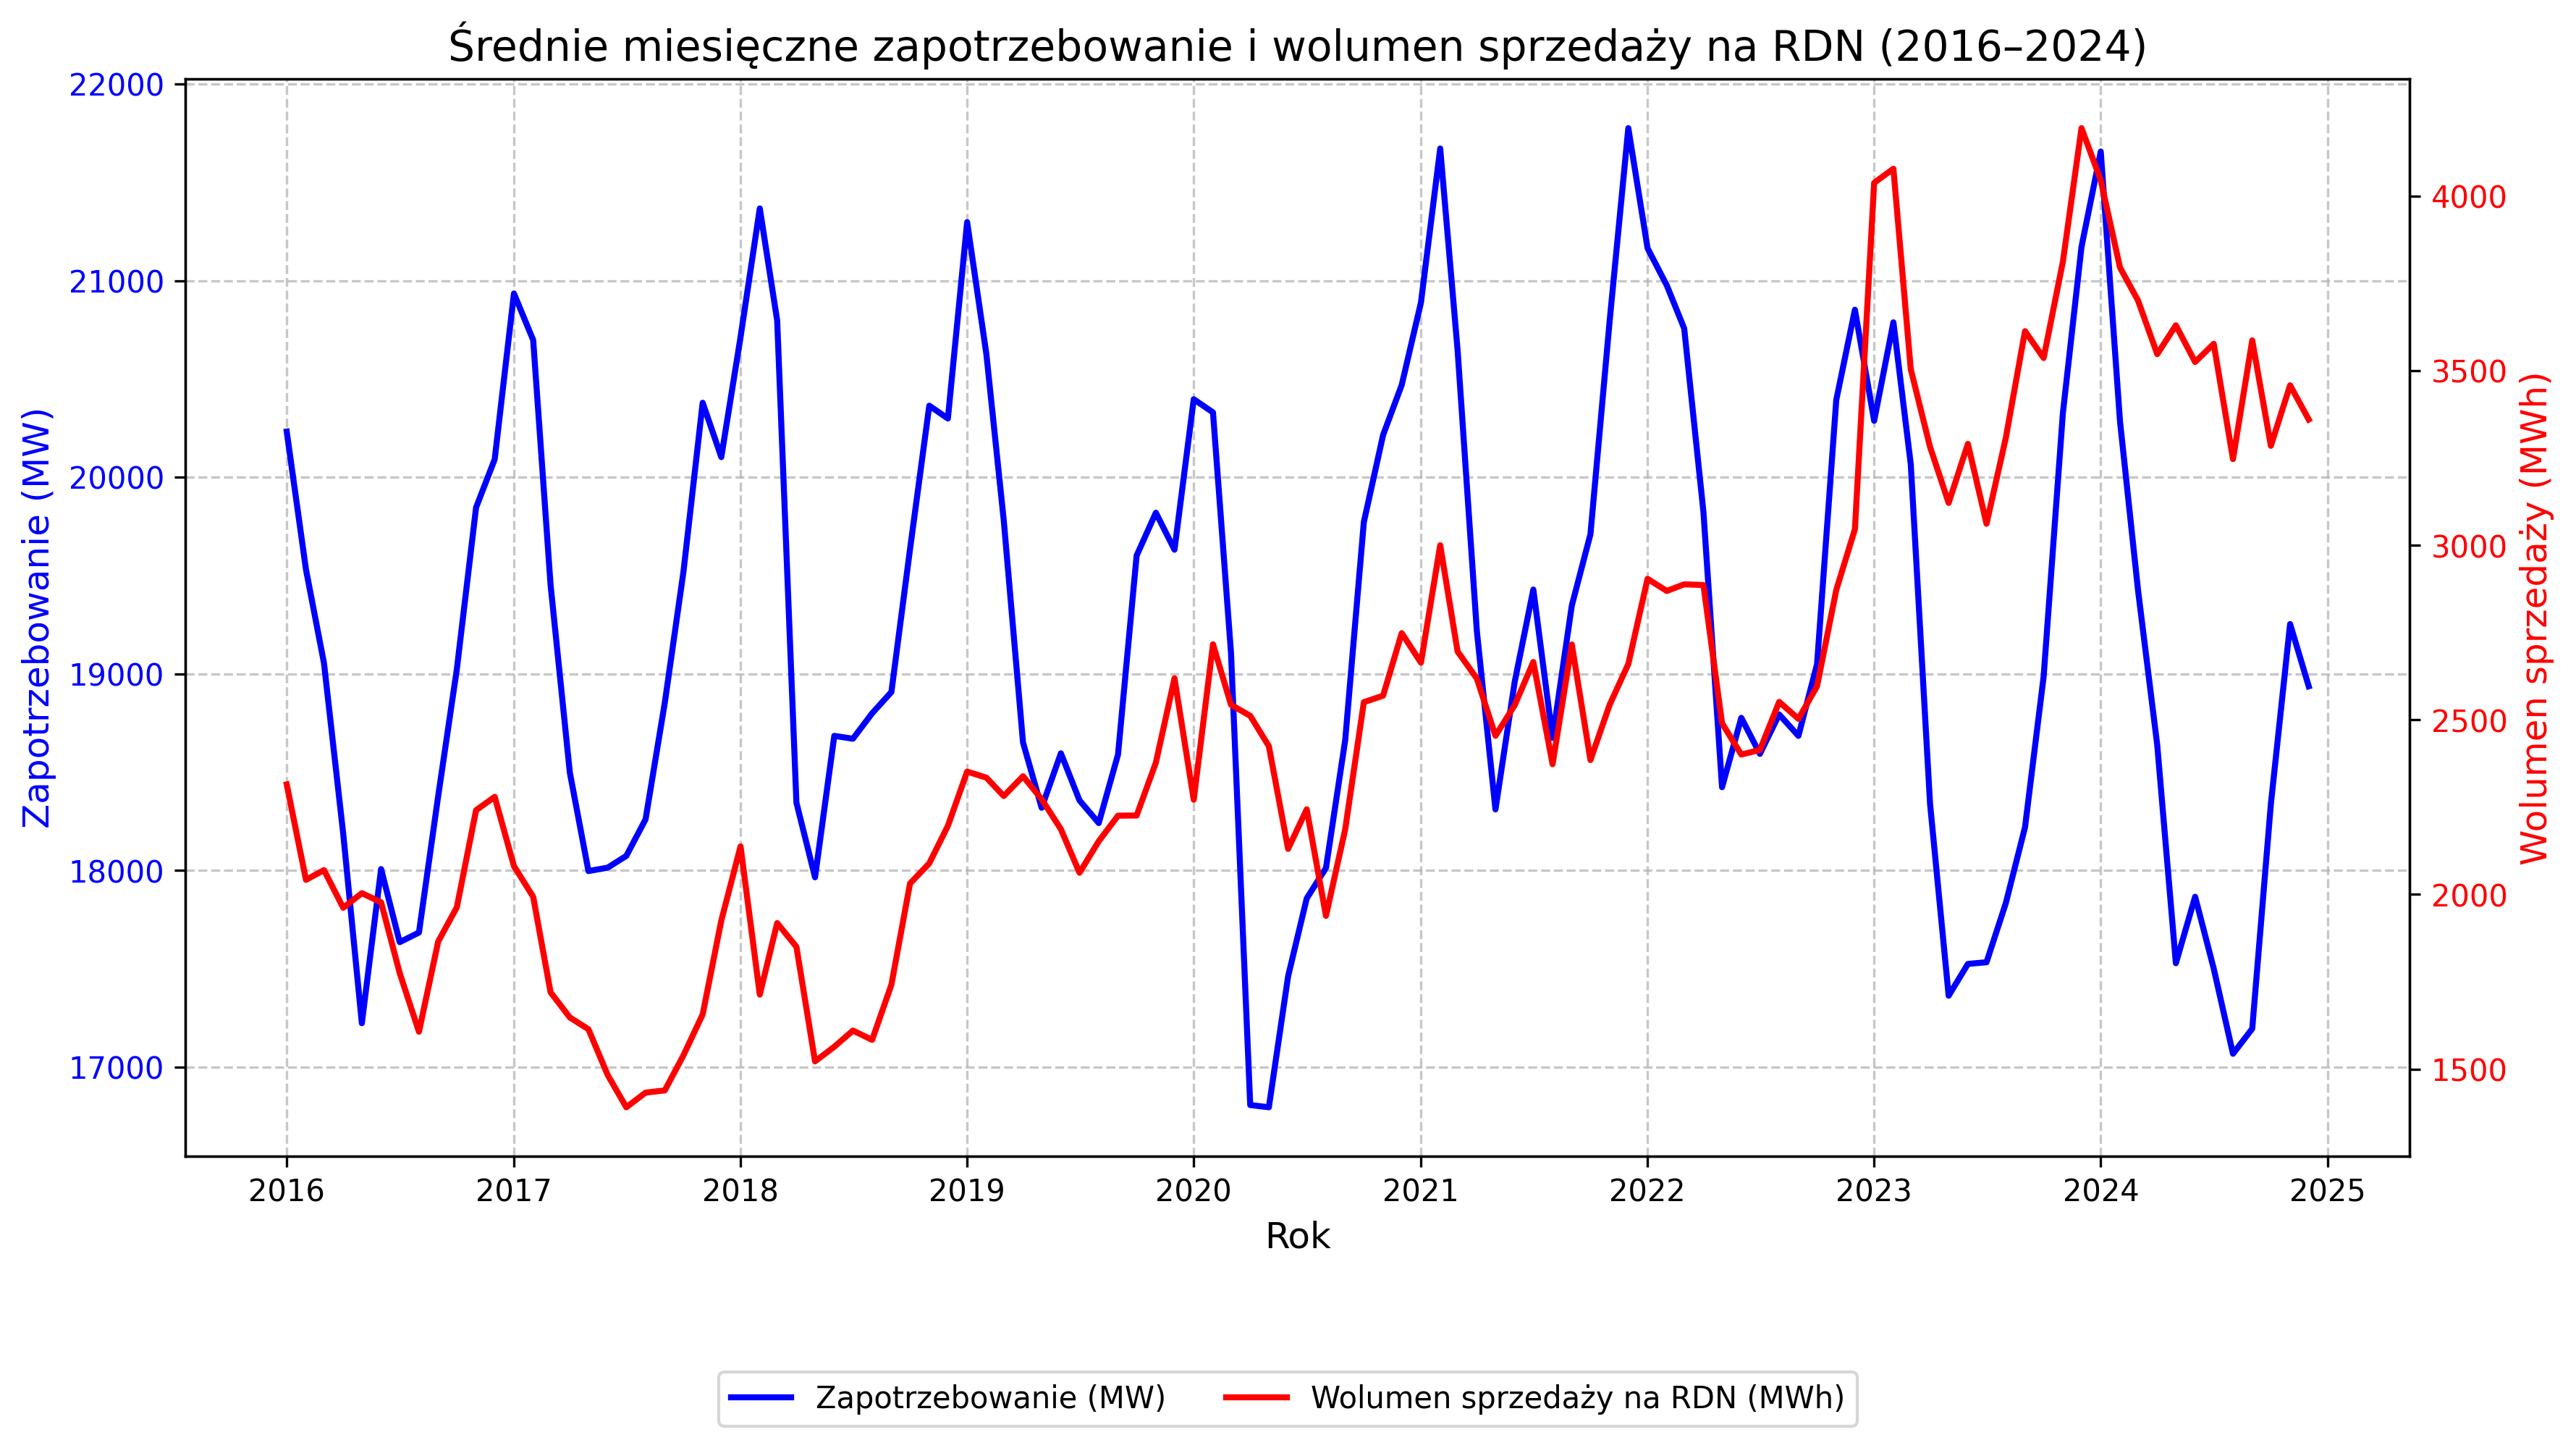
\includegraphics[width=0.9\textwidth]{../plots/market/load_vs_volume_2016_2024.png}
    \caption{Zapotrzebowanie na energię i wolumen handlu w latach 2016-2023 (w ujęciu miesięcznym). Źródło: Opracowanie własne na podstawie danych z PSE.}
    \label{fig:load_vs_trade_volume}
\end{figure}

Rozbieżność między zapotrzebowaniem a wolumenem sprzedaży na RDN ma swój powód. Wolumen sprzedaży na RDN zwykle nie przekracza 5000 MWh. Porównanie do zapotrzebowania na poziomie ponad 15 000  MWh wskazuje, że RDN pokrywa jedynie część całkowitego zapotrzebowania. Pozostała część jest zaspokajana przez: (1) kontrakty bilateralne (OTC), (2) rynek bilansujący, na którym PSE obsługuje zakup oraz sprzedaż energii w czasie rzeczywistym, (3) import energii z sąsiednich krajów, jak pokazano w podrozdziale~\ref{subsec:trade} oraz innego rodzaju transakcje. 

Wyraźnie widoczne są duże szczyty zapotrzebowania zapotrzebowania w okresie zimowym. Wynika to z zwiększonego zapotrzebowania na energię elektryczną w okresie grzewczym, co jest typowe dla klimatu Polski.

\subsection{Rynek bilansujący}
\label{subsec:balancing_market}

Rynek bilansujący odgrywa kluczową rolę w systemie elektroenergetycznym, zapewniając równowagę między podażą a popytem na energię elektryczną w czasie rzeczywistym. W niniejszej analizie uwzględniono zmienną \texttt{RB\_price} (cena na rynku bilansującym w PLN/MWh), pochodzącą z danych Polskich Sieci Elektroenergetycznych (PSE) \cite{PSEOLD}, dostępną w rozdzielczości godzinowej. \gls{rb} służy jako mechanizm korygujący, umożliwiając operatorowi systemu (PSE) zarządzanie nagłymi niedoborami lub nadwyżkami energii, wynikającymi np. z awarii, zmian w zapotrzebowaniu lub fluktuacji produkcji ze źródeł odnawialnych. W przeciwieństwie do Rynku Dnia Następnego (RDN), gdzie ceny ustalane są z wyprzedzeniem (\texttt{fixing\_i\_price}), ceny na rynku bilansującym odzwierciedlają bieżące warunki rynkowe.

Ceny z rynku bilansującego mogą wpływać na ceny RDN, ponieważ różnica między nimi może powodować zmiany w zachowaniach uczestników rynku. Na przykład, jeśli cena na rynku bilansującym jest znacznie niższa niż na RDN, może to skłonić uczestników rynku do zakupu energii na rynku bilansującym, co z kolei wpłynie na ceny na RDN.

W celu oceny różnic cenowych między rynkami przeprowadzono analizę odchyleń ceny na rynku bilansującym (\texttt{rb\_price}) od ceny na RDN (\texttt{fixing\_i\_price}). Obliczone średnie odchylenie na całym zbiorze danych wynosi -7.29 PLN/MWh, co wskazuje, że ceny na rynku bilansującym są średnio niższe niż na RDN w analizowanym okresie (2016-2023). Taka wartość może sugerować efektywność mechanizmów równoważenia w systemie elektroenergetycznym. Dynamikę tych różnic zilustrowano na wykresie poniżej.

\begin{figure}[H]
    \centering
    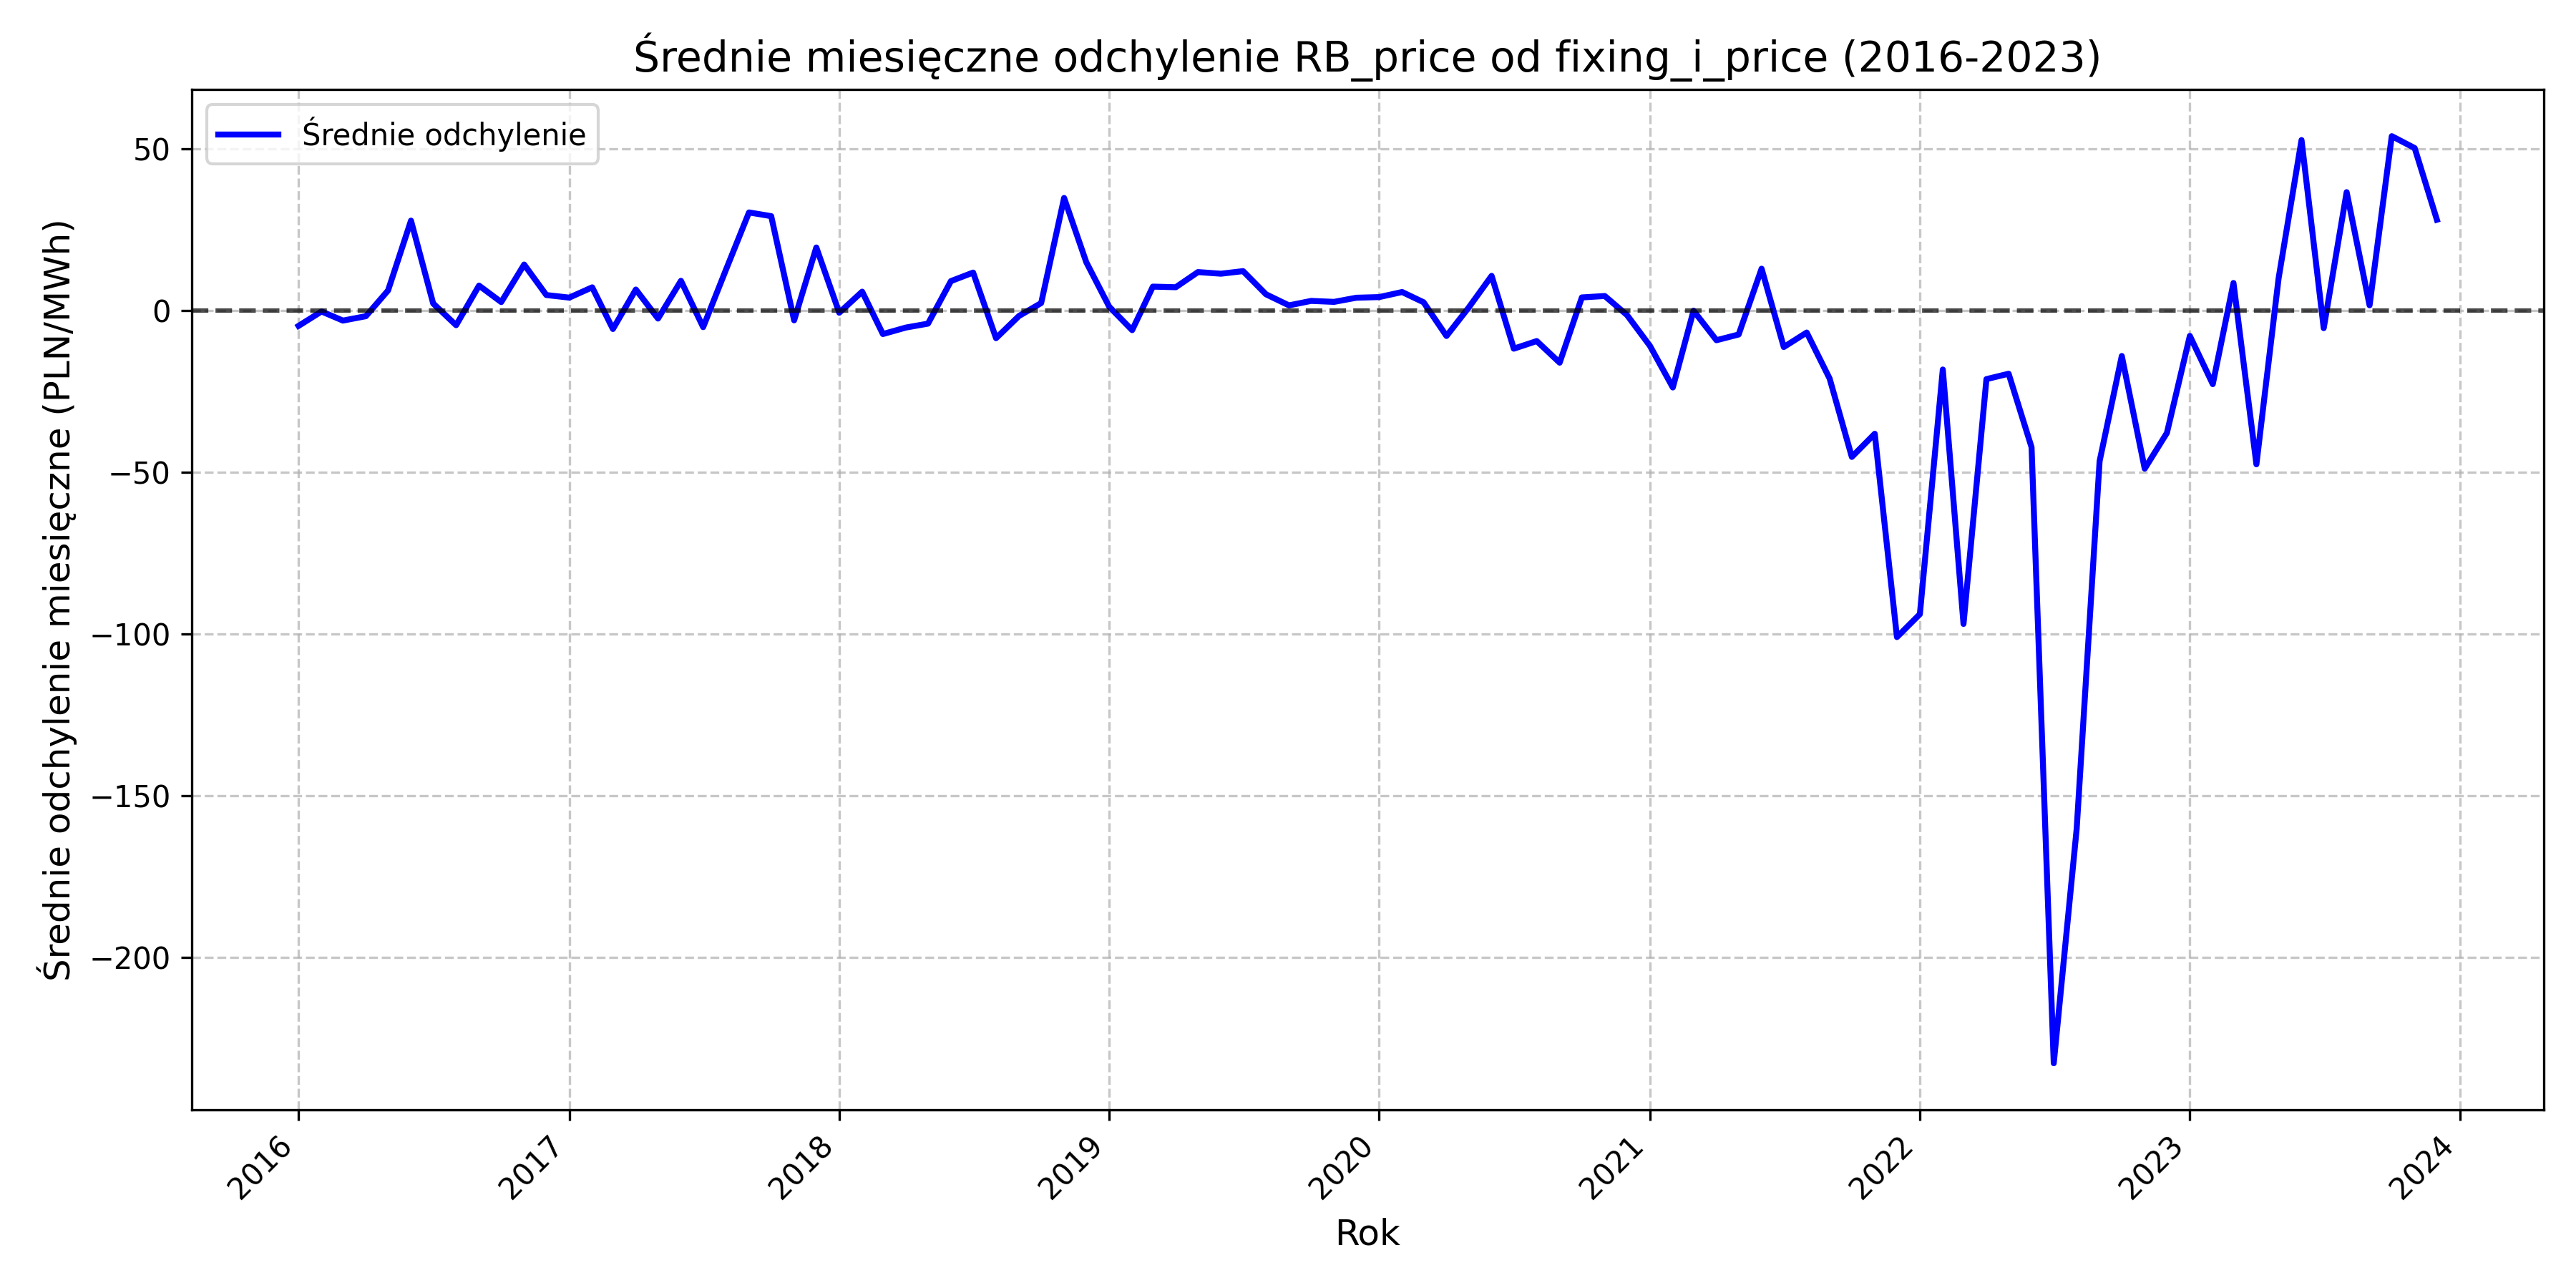
\includegraphics[width=0.9\textwidth]{../plots/market/average_price_deviation.png}
    \caption{Średnie miesięczne odchylenie ceny na rynku bilansującym (\texttt{rb\_price}) od ceny na Rynku Dnia Następnego (\texttt{fixing\_i\_price}) w latach 2016-2023 (w PLN/MWh). Źródło: Opracowanie własne na podstawie danych z PSE.}
    \label{fig:price_deviation}
\end{figure}

W okresach największych wahań cenowych na rynku energii w 2022 roku, ceny na rynku bilansującym niższe niż na RDN. Wartości te mogą być wynikiem większej elastyczności rynku bilansującego, który może szybko reagować na zmiany w zapotrzebowaniu i podaży energii. Wartości ujemne sugerują, że w tych okresach operator systemu mógł być w stanie zaspokoić zapotrzebowanie na energię po niższych kosztach niż te ustalone na RDN.

\subsection{Inne zmienne}
\label{subsec:seasonal}

W swoim zbiorze danych uwzględnione zostały inne zmienne, które mogą mieć wpływ na ceny energii na RDN.

\subsubsection{Zmienne sezonowe}
\label{subsubsec:seasonal_variables}
Zmienne sezonowe, takie jak \texttt{day\_of\_week}, \texttt{month} i \texttt{is\_holiday}, zostały wprowadzone do zbioru danych w celu uchwycenia cykliczności i wzorców sezonowych w cenach energii na Rynku Dnia Następnego.

Zmienna \texttt{month} reprezentuje miesiąc roku (1-12, gdzie 1 to styczeń, a 12 to grudzień). Na temat cykliczności miesięcznej wspominałęm wcześniej w podrozdziałach \ref{subsec:prices} i \ref{subsec:demand}. Niemniej jednak, wprowadzenie zmiennych \texttt{day\_of\_week} i \texttt{month} do modelu pozwala lepiej uchwycić cykliczność i sezonowość w cenach energii, na poszczególne godziny dnia o czym świadczy poniższy wykres korelacji.

Zmienna \texttt{day\_of\_week} reprezentuje dzień tygodnia w zakresie od 1 do 7. Zmienna pozwala uwzględnić modelowi cykliczność tygodniową w cenach energii. Z wykresu poniżej wynika, że zapotrzebowanie na energię jest zazwyczaj wyższe w dni robocze, gdy działa przemysł i biura, a niższe w weekendy i święta, gdy aktywność gospodarcza jest mniejsza. Ta cykliczność przekłada się na ceny energii na RDN: w dni robocze ceny są zazwyczaj wyższe, szczególnie w godzinach szczytu. Wprowadzone zmienne sezonowe pozwalają modelowi lepiej uchwycić te wzorce, co jest istotne w dokładnym modelowaniu.

\begin{figure}[H]
    \centering
    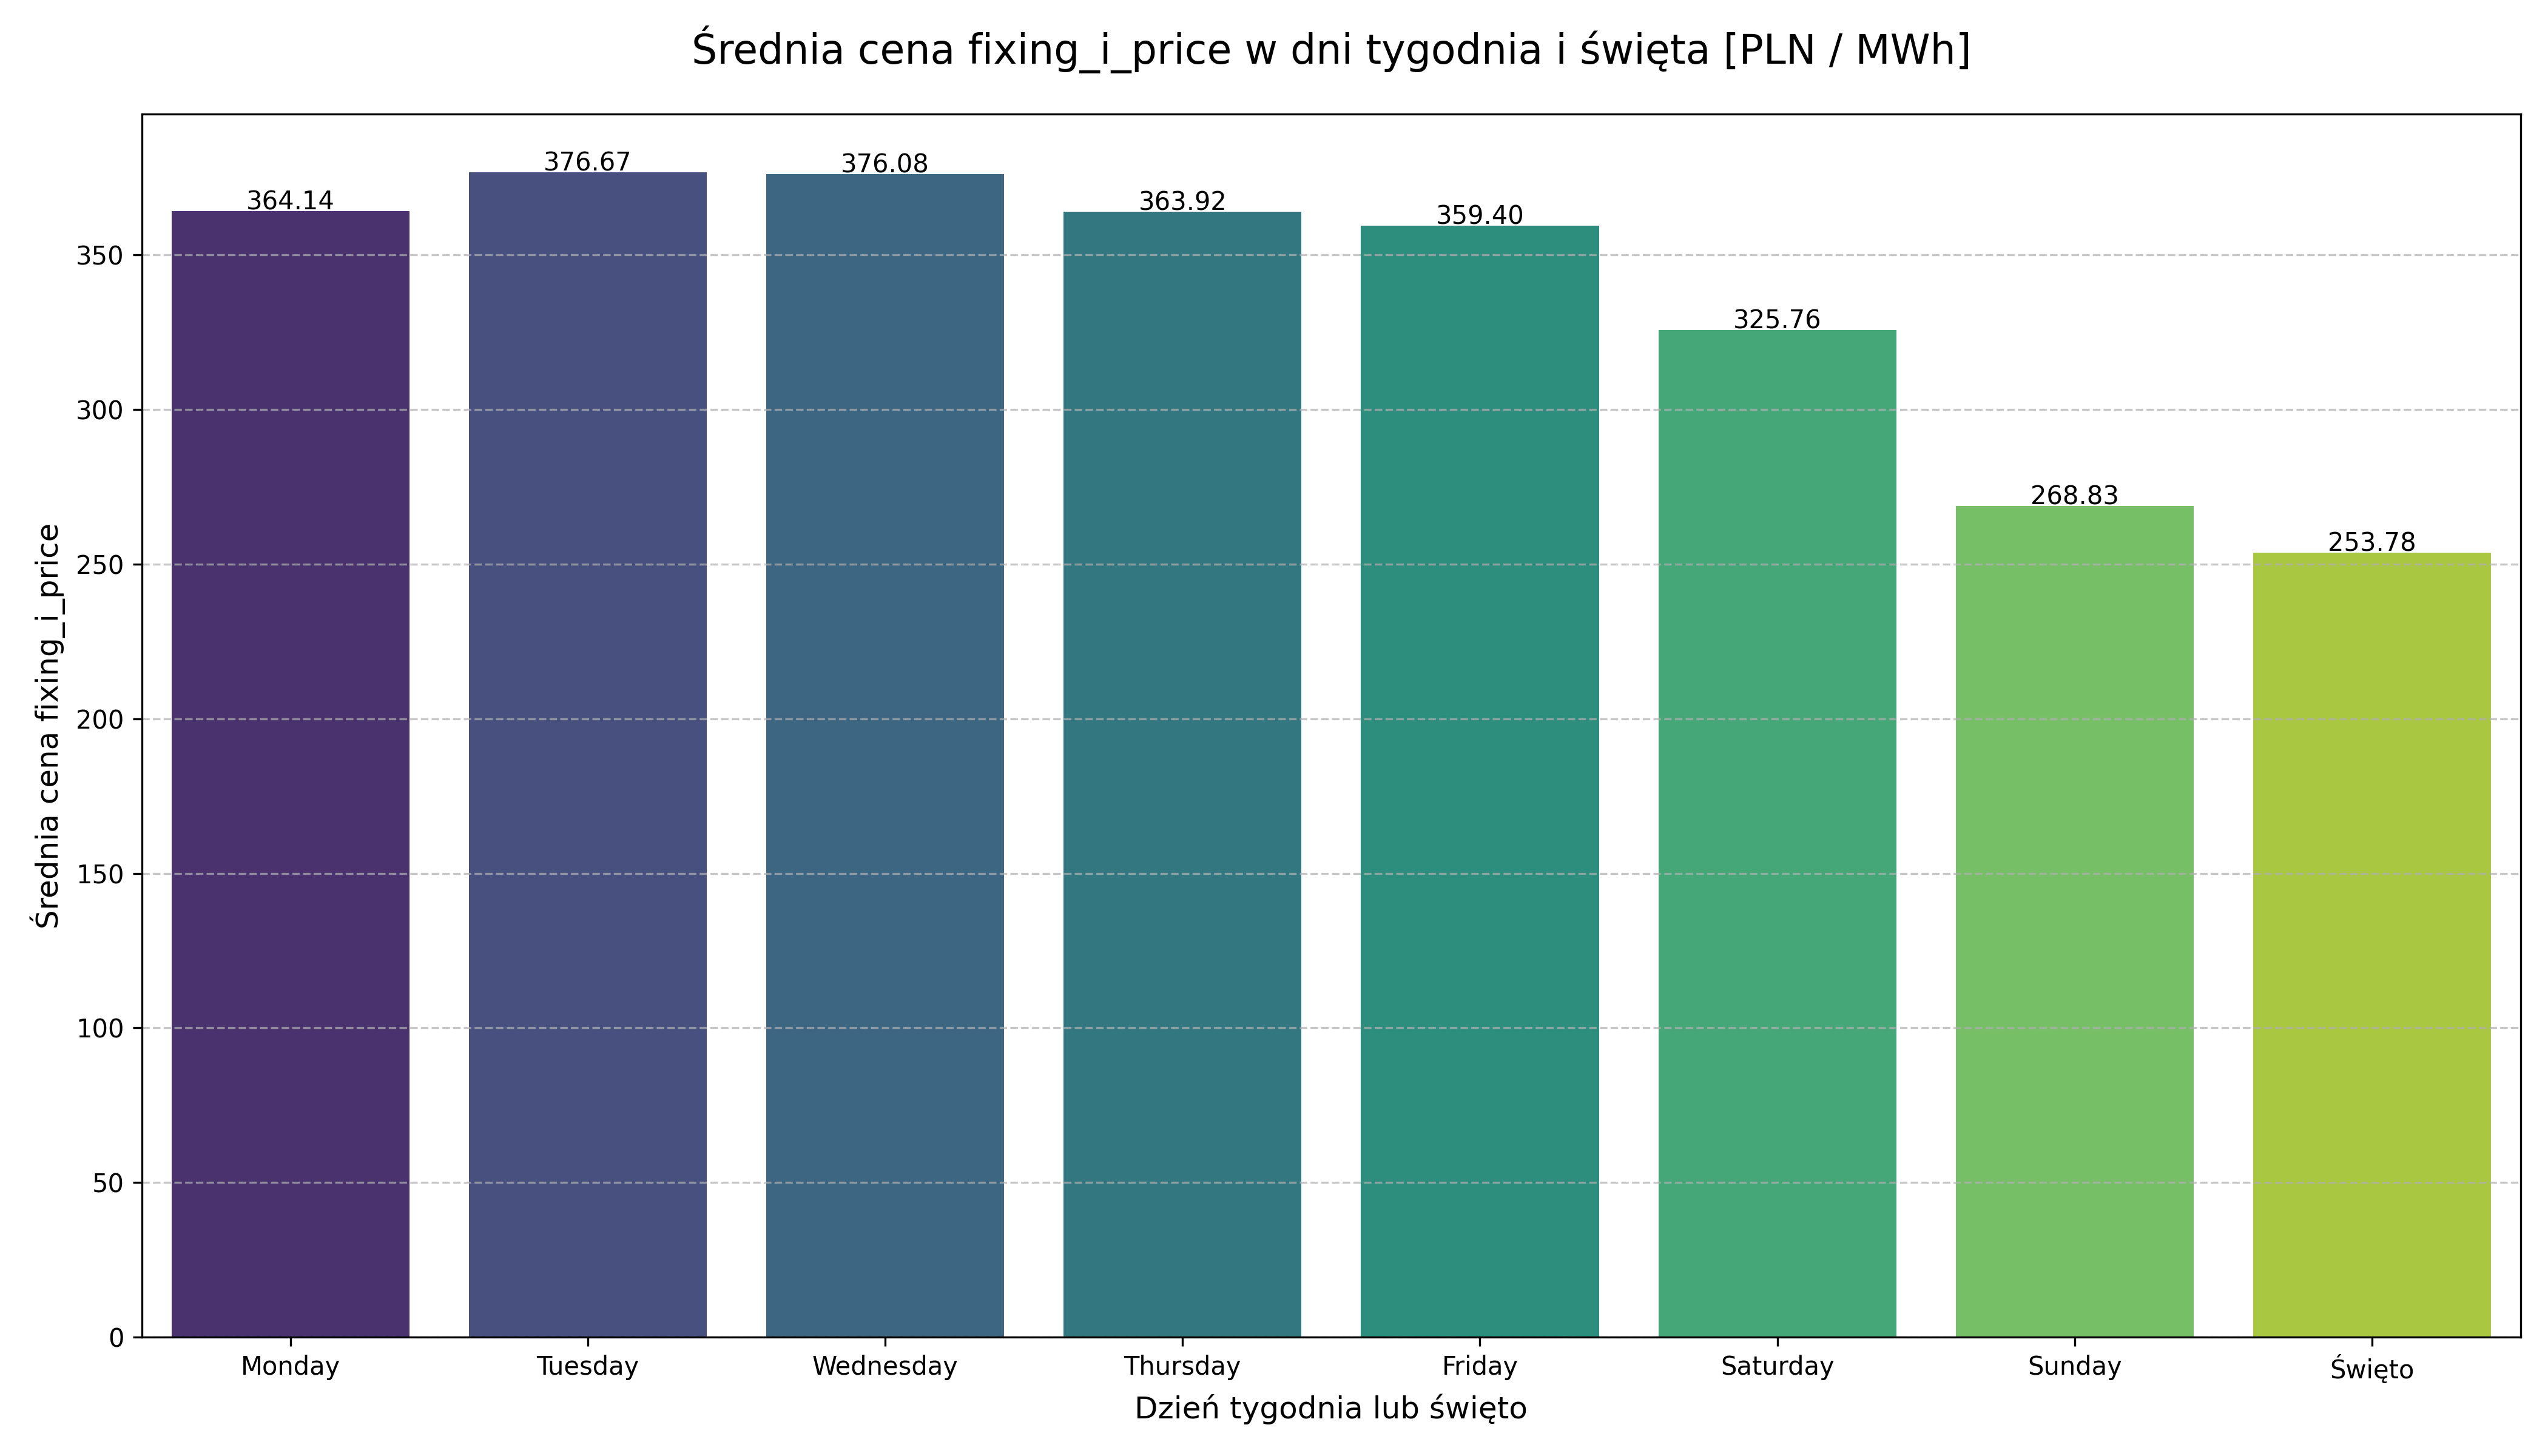
\includegraphics[width=0.9\textwidth]{../plots/fixing_i_price_weekdays_holidays.png}
    \caption{Korelacja dni tygodnia z cenami energii na RDN.}
    \label{fig:seasonal-correlation}
\end{figure}

Dodatkowo wprowadzono zmienną \texttt{peak\_hour}, która jest zmienną binarną określającą godziny szczytu, w których występuje zwiększone zapotrzebowanie na energię elektryczną. Przyjmuje wartość 1, jeśli spełniony jest jeden z dwóch warunków, w przeciwnym razie 0:
\begin{itemize}
    \item W dni wolne lub dni weekendowe, zapotrzebowanie przekracza 18 000 MW, a godzina należy do przedziałów porannych (7:00-9:00) lub wieczornych (16:00-18:00).
    \item W dni robocze, zapotrzebowanie przekracza 23 000 MW i posiada takie same przedziały godzinowe jak w dni wolne.
\end{itemize}
Definicja ta odzwierciedla wyższe zapotrzebowanie na energię w godzinach szczytu, z różnymi progami dla dni roboczych i wolnych, co jest zgodne z charakterystyką polskiego rynku energii.

\subsubsection{Ceny historyczne}
\label{subsec:historical_prices}
 
Zmienne historyczne \texttt{fixing\_i\_price\_lag24}, \texttt{fixing\_i\_price\_lag48}, \texttt{fixing\_i\_price\_lag72}, \texttt{fixing\_i\_price\_lag96}, \texttt{fixing\_i\_price\_lag120}, \texttt{fixing\_i\_price\_lag144} oraz \newline \texttt{fixing\_i\_price\_lag168}, zostały wprowadzone do zbioru danych w celu uchwycenia autokorelacji w cenach energii na RDN. Zmienne te zostały wygenerowane na podstawie kolumny \texttt{fixing\_i\_price}, która reprezentuje cenę energii na RDN w danej godzinie (w PLN/MWh), poprzez przesunięcie wartości o odpowiednią liczbę godzin. 

Dodatkowo, zostały wprowadzone średnie kroczące z ostatnich 24 i 48 godzin. W wyniku tego do datasetu zostały dodane zmienne \texttt{fixing\_i\_price\_mean24} i \texttt{fixing\_i\_price\_mean48}, które reprezentują średnie ceny energii na RDN w ostatnich 24 i 48 godzinach. Wartości te zostały obliczone na podstawie danych z kolumny \texttt{fixing\_i\_price} z przesunięciem o jedną godzinę, żeby nie w średniej kroczącej nie brać pod uwagę obecnej wartości.

Wprowadzenie zmiennych historycznych do modelu pozwala lepiej uchwycić autokorelację i cykliczność w cenach energii, co jest kluczowe dla poprawy dokładności prognoz. Zgodnie z literaturą, ceny historyczne są często jednymi z najważniejszych predyktorów w modelach prognozowania cen energii.

\subsubsection{Kurs wymiany walut}
\label{subsec:waluty}

\subsubsection{Kursy walut}
\label{subsec:exchange-rates}

Zmienne \texttt{pln\_usd} oraz \texttt{pln\_eur} reprezentują odpowiednio kursy wymiany złotego polskiego względem dolara amerykańskiego (USD/PLN) oraz euro (EUR/PLN) w danej godzinie. Dane te zostały pozyskane z oficjalnej strony Narodowego Banku Polskiego (NBP) \cite{NBP_RATES} w granulacji dziennej. W celu dopasowania danych do godzinowego formatu Rynku Dnia Następnego (RDN), wartości kursów zostały przypisane do wszystkich godzin w danym dniu. W przypadku dni wolnych od pracy lub braku dostępnych danych w weekendy lub święta, wartości kursów zostały interpolowane metodą liniową, co pozwoliło na uzyskanie ciągłości danych.

\begin{table}[H]
    \centering
    \begin{tabular}{|c|c|c|}
    \hline
    \textbf{Rok} & \textbf{Średni kurs PLN/USD} & \textbf{Średni kurs PLN/EUR} \\ \hline
    2016 & 3.94 & 4.36 \\ \hline
    2017 & 3.78 & 4.26 \\ \hline
    2018 & 3.61 & 4.26 \\ \hline
    2019 & 3.84 & 4.30 \\ \hline
    2020 & 3.90 & 4.44 \\ \hline
    2021 & 3.86 & 4.57 \\ \hline
    2022 & 4.46 & 4.69 \\ \hline
    2023 & 4.20 & 4.54 \\ \hline
    \end{tabular}
    \caption{Średni kurs wymiany PLN/USD i PLN/EUR w latach 2016-2023. Źródło: Opracowanie własne na podstawie danych NBP.}
    \label{tab:pln-usd-exchange-rate}
\end{table}

Kursy wymiany walut są istotnymi czynnikami w kontekście prognozowania cen energii na Rynku Dnia Następnego, ponieważ wpływają na koszty importu surowców energetycznych oraz handel międzynarodowy. Zmienna \texttt{pln\_usd} jest kluczowa, ponieważ Polska importuje znaczną część paliw kopalnych, takich jak gaz ziemny i ropa naftowa (np. Brent, której cena jest wyrażona w dolarach amerykańskich i przeliczona na PLN w zmiennej \texttt{brent\_price}). Wzrost kursu PLN/USD, czyli osłabienie złotego względem dolara, zwiększa koszty importu tych surowców, co może prowadzić do wzrostu kosztów produkcji energii, a w konsekwencji do wyższych cen na RDN.

Z kolei zmienna \texttt{pln\_eur} odgrywa istotną rolę w kontekście handlu energią z krajami sąsiednimi, ponieważ ceny energii na rynkach europejskich, takich jak Czechy (\texttt{cz\_price}), Słowacja (\texttt{sk\_price}), Litwa (\texttt{lt\_price}) czy Szwecja (\texttt{se\_price}), są wyrażone w euro. W niniejszej analizie ceny te zostały przeliczone na złotówki przy użyciu kursu \texttt{pln\_eur}, co pozwoliło na ujednolicenie jednostek walutowych i bezpośrednie porównanie z cenami na polskim RDN (\texttt{fixing\_i\_price}). Wahania kursu PLN/EUR mogą wpływać na decyzje dotyczące importu lub eksportu energii - na przykład, osłabienie złotego względem euro zwiększa koszt importu energii z rynków sąsiednich, co może podnieść ceny w Polsce.

Kursy polskiego złotego odzwierciedlają również zmiany w gospodarce krajowej i globalnej. Próbując stabilizować kurs, Narodowy Bank Polski zmienia politykę monetarną kraju, co może wpływać na koszt produkcji energii (np. poprzez zmiany stóp procentowych, które oddziałują na koszty finansowania inwestycji energetycznych). W efekcie zarówno kurs PLN/USD, jak i PLN/EUR mają pośredni wpływ na dynamikę cen energii na Rynku Dnia Następnego.